\chapter{The \lhcb experiment} 
\label{ch:detector}
\minitoc


This chapter describes the \lhcb experiment; including both the accelerator complex responsible for providing \proton\proton collisions and the \lhcb detector itself.  
The \lhcb experiment is a collaboration of around 800 scientists from 72 different institutions in 16 countries. The primary physics goal is to look for indirect signs of New Physics in heavy flavour decays. The experiment is situated on the Large Hadron Collider at CERN, Geneva. 



\section{\cern and the \lhc}


In the aftermath of the Second World War a number of eminent scientists proposed the creation of a collaborative European laboratory dedicated to the study of atomic physics. With this, the `Conseil Europ\'een pour la Recherche Nucl\'eaire' was born; a provisional council set up in 1952 to oversee the laboratory's creation.  The organisation as it is today was established in 1954, renamed the `Organisation Europ\'eenne pour la Recherche Nucl\'eaire', although the acronym \cern remained. 
The purpose of \cern was clear; the convention dictates that the organisation \emph{`shall provide for collaboration among European States in nuclear research of a pure scientific and fundamental character'}.
Since then \cern has been a hub of fundamental nuclear and particle physics research, producing a number of Nobel Prize-winning discoveries, alongside technological developments benefiting society as a whole.

The convention stipulates that the organisation \emph{`shall have no concern with work for military requirements'} and  
requires \emph{`the results of its experimental and theoretical work shall be published or otherwise made generally available'}. 
The choice of the laboratories location followed a similar set of values, picking Geneva, Switzerland owing both to the central European location and neutrality of the host state. 


Perhaps currently the most well known accelerator in the complex, \cern is home to the Large Hadron Collider (\lhc). Two beams of hadrons circulate in opposite directions around 27\km rings, colliding at four interaction points. The beam pipes and experimental halls are buried deep underground, providing shielding from cosmic radiation and reducing the cost of acquiring large areas of land. The tunnels traverse the Franco-Swiss border at a depth that varies between 50--175\m at the shallowest and deepest points respectively.      

The tunnel and caverns occupied by the \lhc pre-date the current accelerators and experiments. There were originally constructed for the Large Electron Positron Collider (\lep)~\cite{Myers:1991ym}. This machine begin operation in 1989 and collided electrons and positrons at a collision energy of $\sqrt{s}=209\gev$.  

% {\color{Red}
% \begin{itemize}
% %\item Founding of \cern and a little history 
% \item LEP was in tunnel before
% %\item Mission statement
% %\item Notable results and and contributions to society
% %\item Mention experiments other than those attached to accelerator complex
% %\item Time line
% \item running periods? and future plans...
% \end{itemize}
% }

\subsection{The accelerator complex}

The \lhc is only one of a vast collection of accelerators at \cern, albeit the largest. The hadrons collided in the \lhc travel sequentially through a number of different machines, boosting their energy in each. The full complex is shown in Fig.~\ref{fig:Dec_lhcb_Schematic} along with a legend detailing the types of particles considered. The protons begin life in a hydrogen gas canister. The gas is ionised and accelerated in  a linear accelerator, LINAC2, to an energy of 50\mev. These then pass into the Proton Synchrotron Booster, raising the energy further from 50\mev to 1.4\gev. 

%%%%%%%%%%%%%%%%%%%%%%%%%%%%%%%%%%%%%%%%%%%%%%%%%%%%%%%%%%
\begin{figure}[!h]
    \centering
    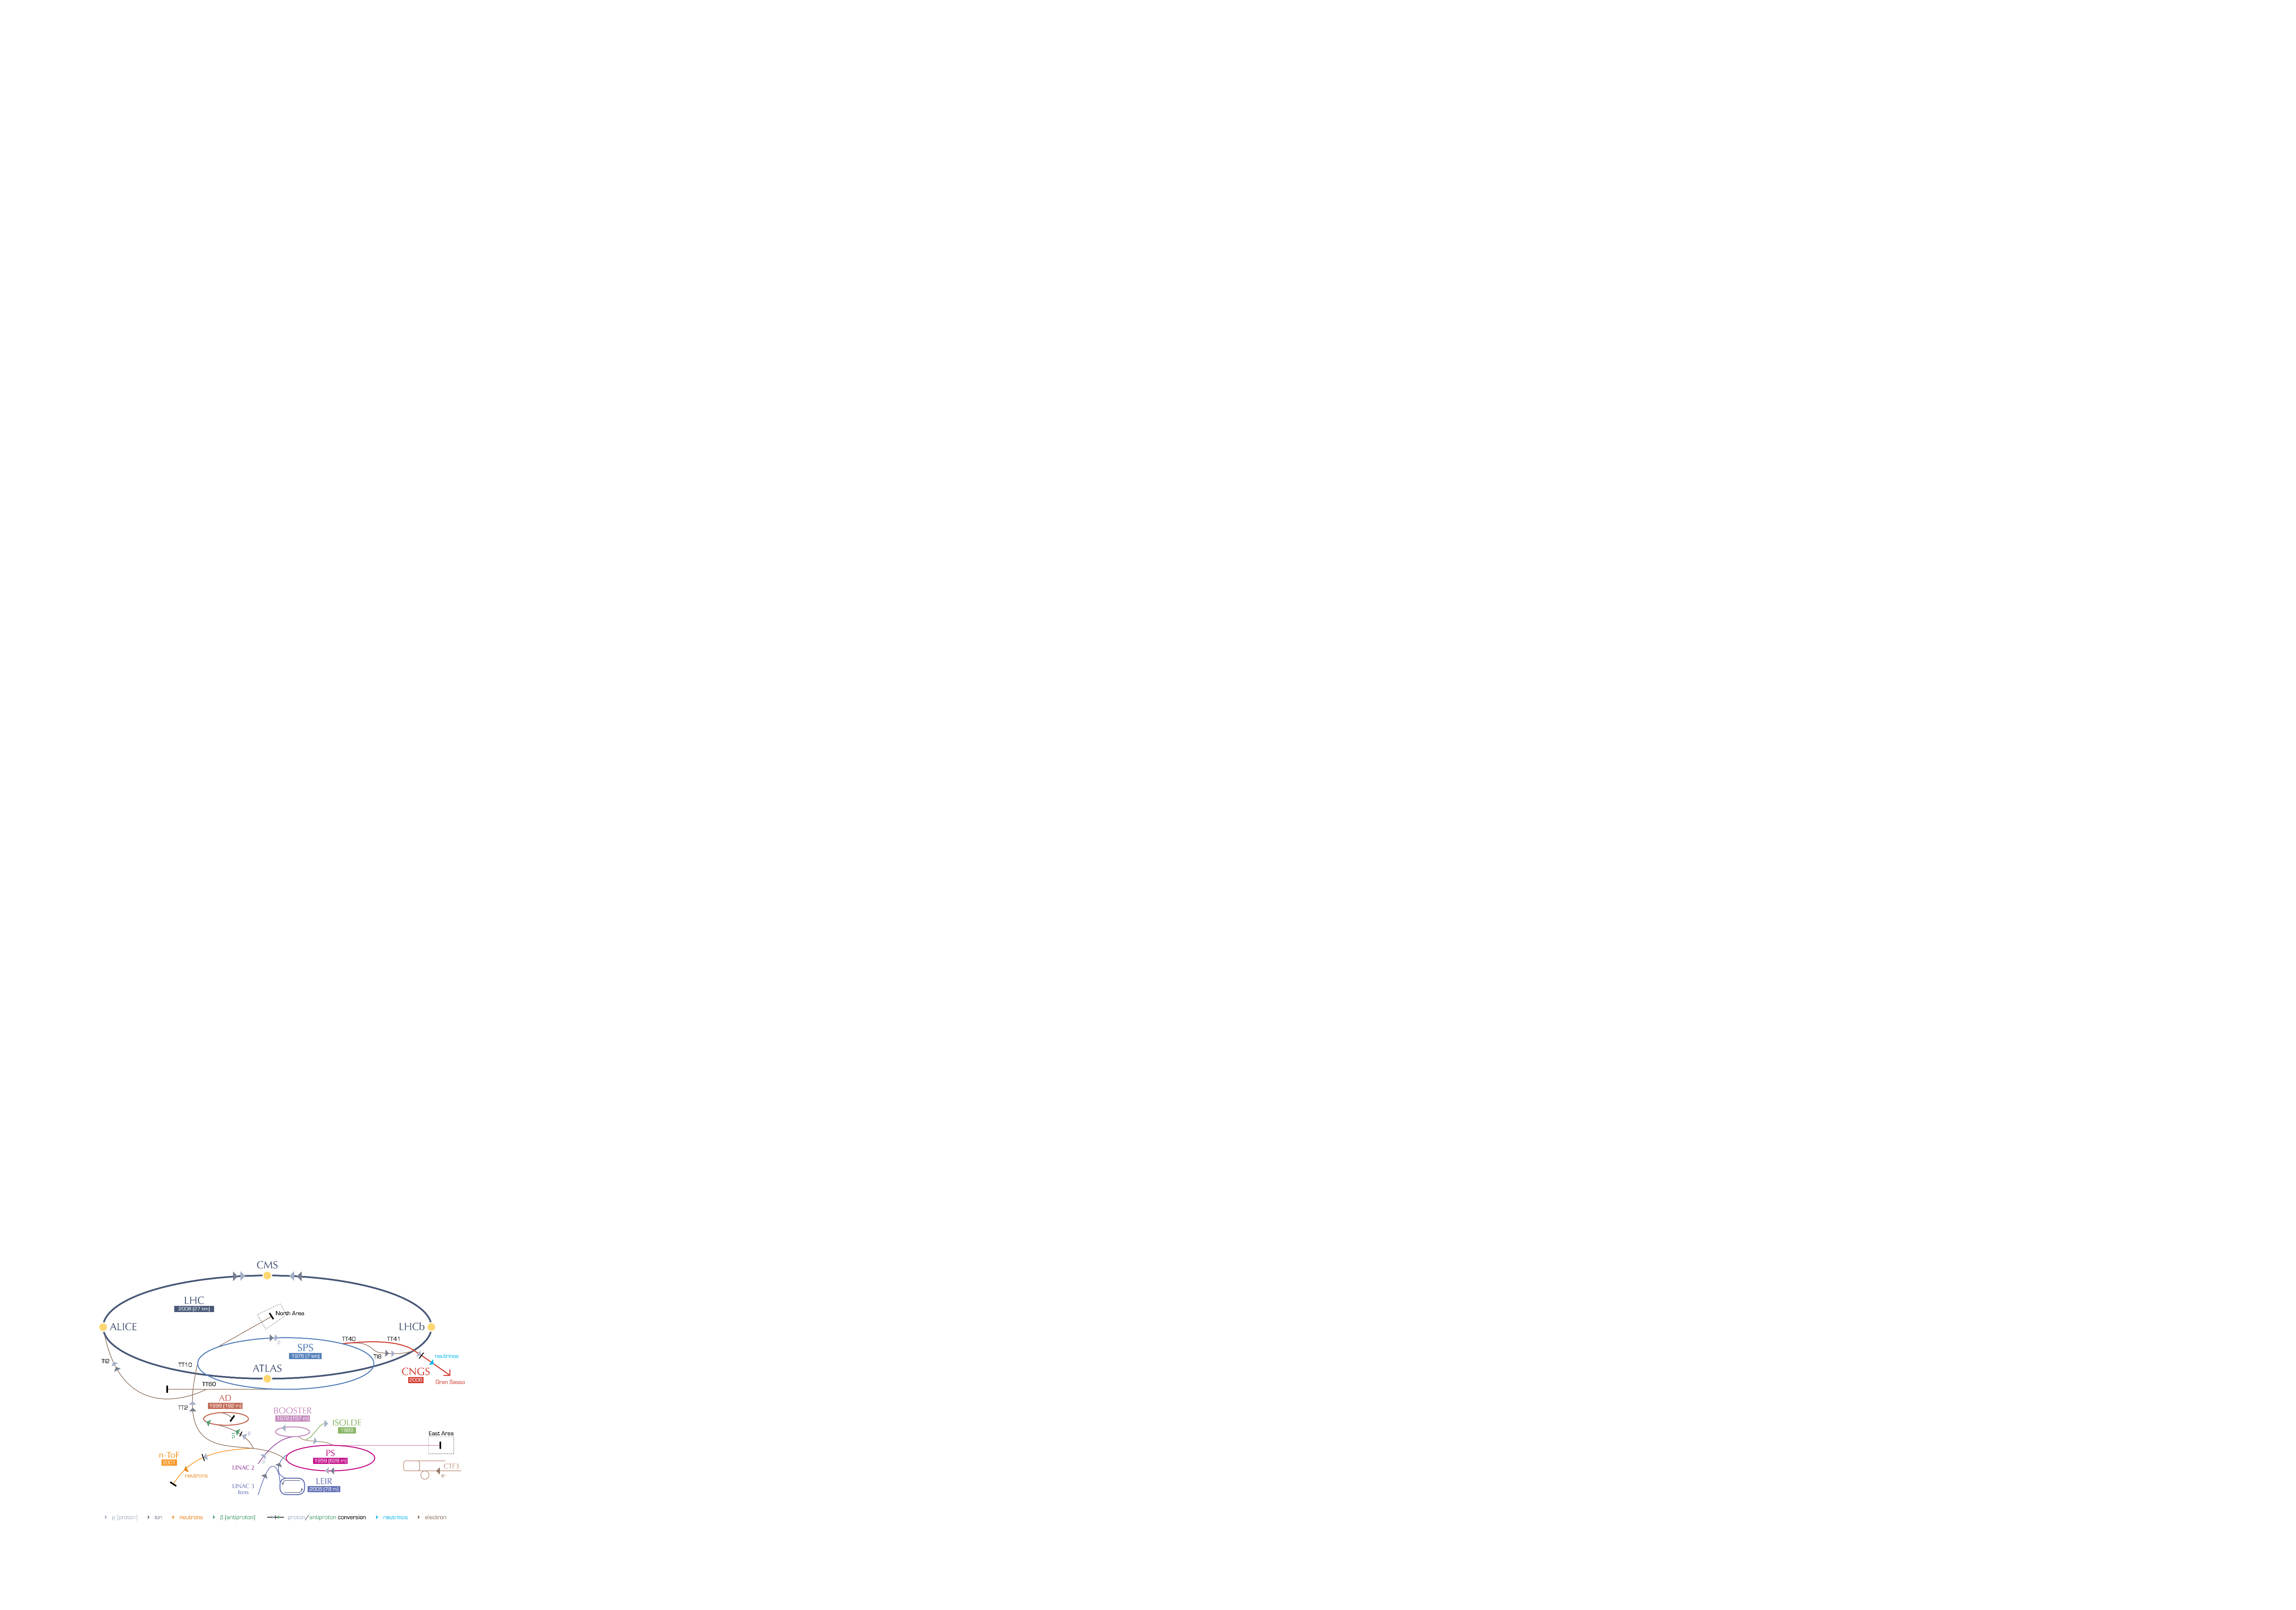
\includegraphics[width=1.0\textwidth]{figs/Detector/Acc_complex.pdf}
    \caption{The accelerator complex at \cern, from~\cite{DeMelis:2119882}.}
    \label{fig:Dec_Acc_Complex}   
\end{figure}
%%%%%%%%%%%%%%%%%%%%%%%%%%%%%%%%%%%%%%%%%%%%%%%%%%%%%%%%%%

In addition to protons, the complex can accelerate other ions including lead, and more recently, xenon. These start in a dedicated linear accelerator, LINAC3, where the electrons are stripped off the ions to produce bare nuclei before being injected into the Low Energy Ion Ring (LEIR). This ring raises the ion's energy from 4.2\mev to 72\mev. 

Either protons or ions can then be injected in the Proton Synchrotron (PS), \cern's first synchrotron. Once the world's highest energy particle accelerator, this now accelerates the particles up to 25\gev ready to be injected into the Super Proton Synchrotron (SPS).
The SPS is the second largest accelerator at \cern, with a circumference of 7\km. It was switched on in 1976 and resulted in the notable discoveries of the \W and \Z bosons. Here, the particles are finally accelerated up to an energy of 450\gev, ready for injection into the \lhc. The particles are transferred from the SPS to the \lhc via two lines, one for each of the \lhc beam directions. The two beams, referred to as Beam 1 and Beam 2, travel clockwise and anti-clockwise respectively when viewed from above. Beam 2 is injected just before the \lhcb detector. 

The particles travel through the accelerator complex in groups called bunches. These typically contain around $10^{11}$ protons and are necessary as a result of the Radio-frequency (RF) cavities that accelerate the particles. The bunches are sequentially transferred between the accelerators in collections called trains. The bunch-trains are transferred from the SPS to the \lhc in a series of injections. Although the \lhc has a capacity for 3465 bunches, the nominal operating conditions has only 2808 of these spaces filled. 
These extra gaps allow enough room to safely divert the direction of the beam, without unintentionally damaging the instrumentation around the beam-pipe. The turn-on time for the magnets responsible for dumping the beam in emergencies is longer than the nominal 25\ns bunch spacing. 


Once the \lhc is filled the beams are accelerated from the injection energy of 450\gev to the nominal energy of up to 7\tev. This is achieved using eight RF cavities per beam to increase the beam energies and 1232 superconducting dipole magnets that bend the trajectory of the charged particles, ensuring they follow the paths dictated by the approximately circular tunnels. The 15\m long dipole magnets contain superconducting niobium-titanium cables, kept at 1.9\,K using super-fluid helium. The 11,850\,A current flowing through the magnets generates a large magnetic field of 8.33\,T. The current is gradually and synchronously ramped as the particles are accelerated, such that the same orbital trajectory is maintained. 

The \lhc contains a wealth of other magnets, another 8,361 in addition to the dipole magnets, that optimise the orbit of the beams. These ensure the beams remain tightly packed together, as well as correcting many higher order perturbations.   

During the injection and acceleration phase no collisions take place. Once the beams are at the nominal energy and profile distribution have been optimised, the two beams are brought together at four interaction points around the ring. Magnets are used to both redirect the beams such that they crossover and to squeeze the beams to a smaller cross-section at the collision points, increasing the likelihood of collisions. Once the beams overlap and the particles collide the experiments located around the four interaction points can begin to record data. The collisions typically continue for a duration of 10--20\hr (referred to as a fill). The number of particles in the bunches reduce, or \emph{burn-off}, as they collide with one another and the beam-pipes. A fill ends when the beams are intentionally dumped, when the number of protons in each bunch gets too low, or automatically dumped, to ensure the safety of the machine. The beam dumps are large graphite blocks surrounded by concrete shielding, designed to absorb the energy of the beams.  

%A total of seven experiments are located at the \lhc, situated in four caverns. The four largest are \atlas, \cms, \lhcb and \alice. The TOTEM, LHCf and MoDEL experiments are located in the same caverns as \cms, \atlas and \lhcb respectively. 


%\subsection{The \lhcb collaboration} 



\subsection{Beam conditions}
\label{sec:Dec_beam_conds}
The beam conditions at the \lhc have varied between the different years of data taking included in this thesis. A summary of some key parameters are detailed in Table~\ref{tab:Dec_phys_params}. This also includes the nominal conditions for the \lhc, for which it was designed. 


\begin{table}[h]
    \centering
      \begin{tabular}{lcccc|c}
         \hline
         Condition                                      & 2011      & 2012      & 2015      & 2016      & Nominal   \\ 
         \hline
         $\sqrt{s}$ (\tev)                              & 7         & 8         & 13        & 13        & 14        \\ 
         \lhc peak luminosity ($10^{33}\cm^{-2} \sec^{-1}$)  & 3.5       & 7.6       & 4.8       & 14        & 12        \\ 
         Bunches                                        & 1380      & 1380      & 1368      & 2736      & 2808      \\ 
         Bunch spacing (\ns)                            & 50        & 50        & 25        & 25        & 25        \\ 
         \hline
         Peak luminosity at \lhcb ($10^{32}\cm^{-2} \sec^{-1}$) & 4.0       & 4.0       & 3.5       & 3.5       & 2--4   \\ 
         Average $N_{\text{collisions}}$, $\mu$         & 1.7       & 1.7       & 1.1       & 1.1       & -         \\ 
         Integrated luminosity (\invfb)                 & 1.0       & 2.0       & 0.3       & 1.5       & -         \\ 
         \hline
      \end{tabular}
   \caption{Beam conditions in the different datasets used in this thesis. The last three rows are specific to \lhcb.}
   \label{tab:Dec_phys_params}
\end{table}


During a normal fill the luminosity delivered to the large experiments slowly decreases as the protons burn off. For the high-\pt experiments, \atlas and \cms, the average number of collisions per bunch crossing (known as pile up) is high: around an average of 27 in 2016. 
For the \lhcb experiment, the average number of visible collisions per bunch crossing, $\mu$, is much lower, between 1.1 and 1.7 depending on the year. The same luminosity is maintained for the majority of a fill via a process know as luminosity levelling. At the beginning of the fill the two beams are vertically separated from one another such that the overlap between them is not maximised. As the fill progresses the two beams are brought closer together to compensate for the burn off of the bunches. This way a constant instantaneous luminosity of between (2--4)$\times 10^{32} \cm^{2} \sec^{-1}$ can be maintained thorough out the given fill. This gives the desired $\mu$.

The two beams collide at an angle in the horizontal plane. This helps to reduce unwanted collisions between the bunches either side of the intended collision bunches. The angle of collision depends on the polarity of the \lhcb spectrometer magnet as the dipole field affects beam-steering fields around the interaction point. 


% {\color{Red}
% \begin{itemize}
% \item \lhc optics
% \item crossing angle
% \end{itemize}
% }


\section{The \lhcb detector}

This section provides an overview of the experimental apparatus used to obtain the data analysed in this thesis.
The \lhcb detector~\cite{Alves:2008zz} is comprised of distinct sub-detectors, each with a dedicated purpose. These help to characterise the sub-atomic particles created in the proton-proton collisions, and enable measurements of their kinematics, trajectories and species.
This overview includes a description of the sub-detector's principles, components and performance. 

The \lhcb detector is found at Point 8 of the \lhc ring, in a cavern originally built for the \delphi detector during the \lep era. A schematic representing the key components of the \lhcb detector is shown in Fig.~\ref{fig:Dec_lhcb_Schematic}. This figure displays the axes convention adopted by \lhcb, and used henceforth. The horizontal axis is labelled the $z$-axis and is parallel to the direction of the beams. The figure's vertical axis is the $y$-axis, increasing as one moves from the cavern up to ground level. The $x$-axis is in the dimension perpendicular to the plane of the figure and increases as one moves towards the centre of the \lhc ring. The counter-rotating beams of protons are collided at the left of this figure inside the Vertex Locator, at the origin in these coordinates.   

%%%%%%%%%%%%%%%%%%%%%%%%%%%%%%%%%%%%%%%%%%%%%%%%%%%%%%%%%%
\begin{figure}[!h]
    \centering
    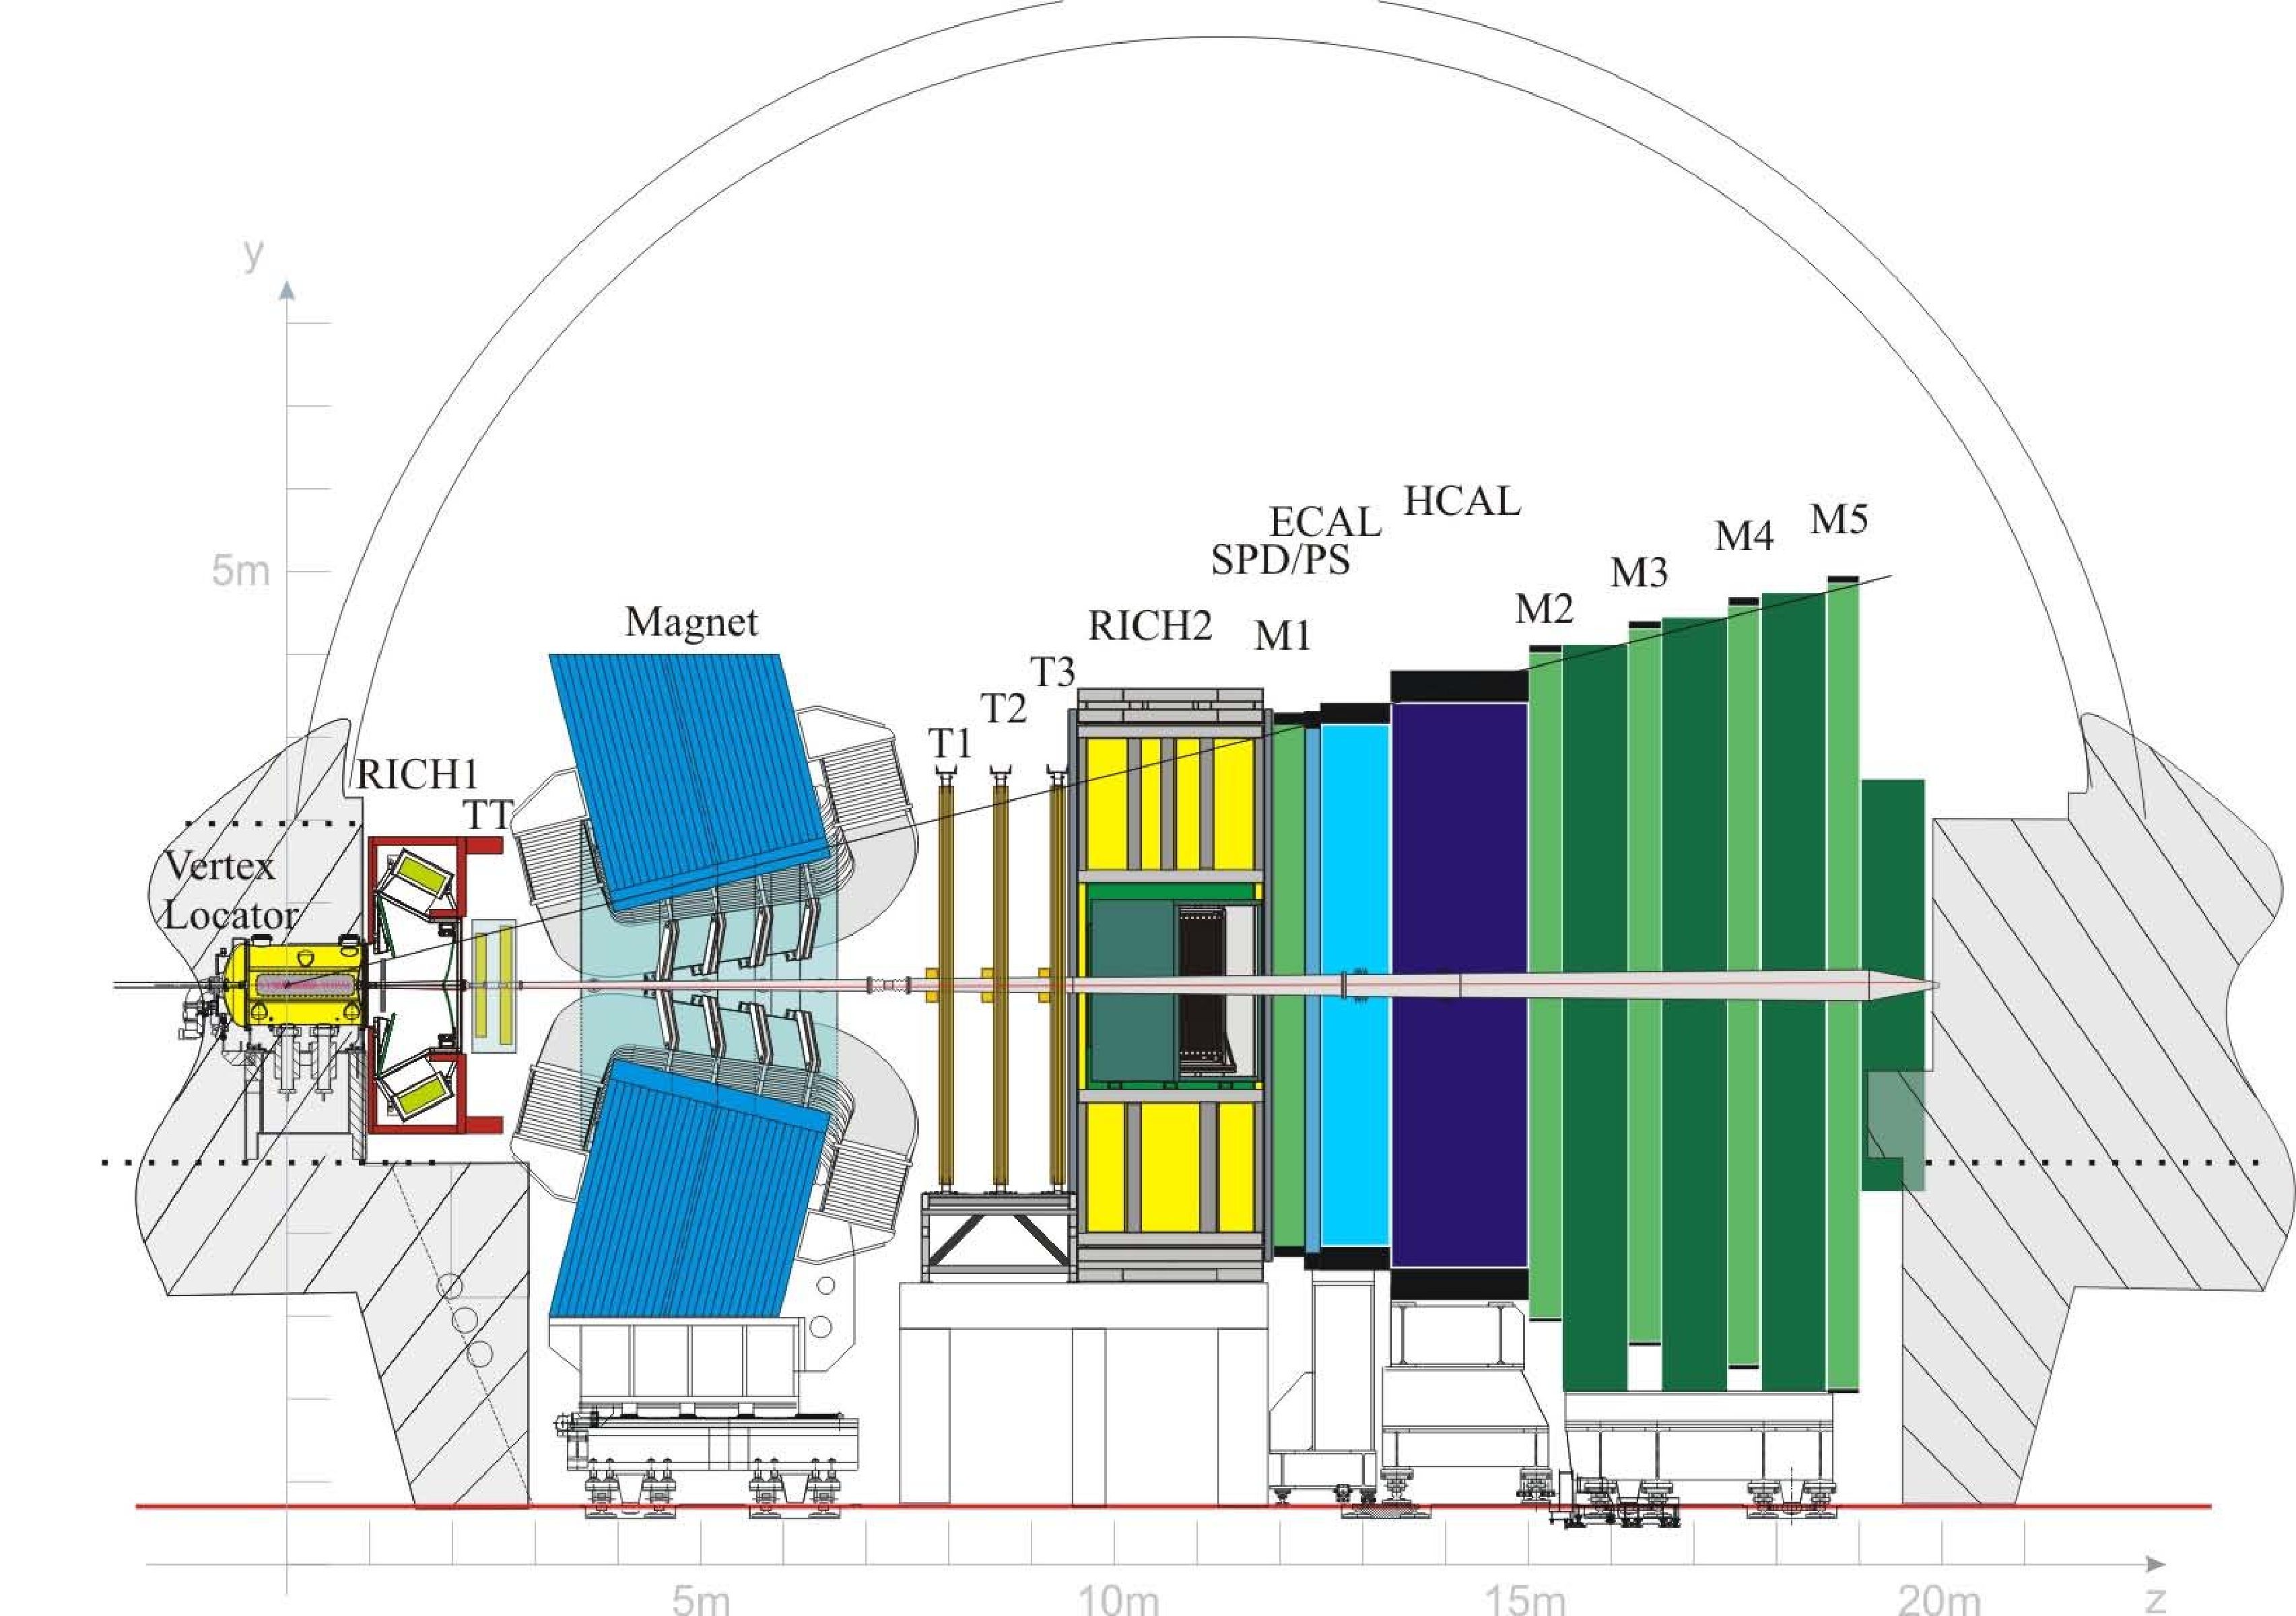
\includegraphics[width=1.0\textwidth]{figs/Detector/LHCb_Detector_Schematic.pdf}
    \caption{Schematic of the \lhcb detector, from Ref.~\cite{Alves:2008zz}. This figure shows the positions of the vertex locator, ring imaging Cherenkov detectors (\richone and \richtwo), magnet, calorimeter systems (\ecal, \hcal, \spd/\presh) and Tracker Turicensis (\ttracker). The sub-detectors labelled T1, T2 and T3 jointly make up the Inner Tracker (\intr) and Outer Tracker (\ot). The sub-detectors labelled M1, M2, M3, M4 and M5 constitute the Muon system.  }
    \label{fig:Dec_lhcb_Schematic}   
\end{figure}
%%%%%%%%%%%%%%%%%%%%%%%%%%%%%%%%%%%%%%%%%%%%%%%%%%%%%%%%%%

The \lhcb detector covers only a small fraction of the solid angle around the collision region; the acceptance covers particles with a pseudo-rapidity in the range $1.8 < \eta < 4.9$ on one side of the interaction point.\footnote{The pseudo-rapidity is related to the polar angle $\theta$ as $\eta\equiv-\log(\tan{(\theta/2)}$.} However, this configuration is well suited to the reconstruction of heavy quark particles. The angular distribution of \bquark\bquarkbar pairs is shown in Fig.~\ref{fig:Dec_bb_production}, along with the acceptance of \lhcb in red. The distribution is highly peaked towards the forward and backward regions as \bquark-hadrons tend to receive large boosts at this collision energy. Approximately 25\% of decays have both \bquark and \bquarkbar quarks produced inside the acceptance.

% %%%%%%%%%%%%%%%%%%%%%%%%%%%%%%%%%%%%%%%%%%%%%%%%%%%%%%%%%%
\begin{figure}[!h]
    \centering
    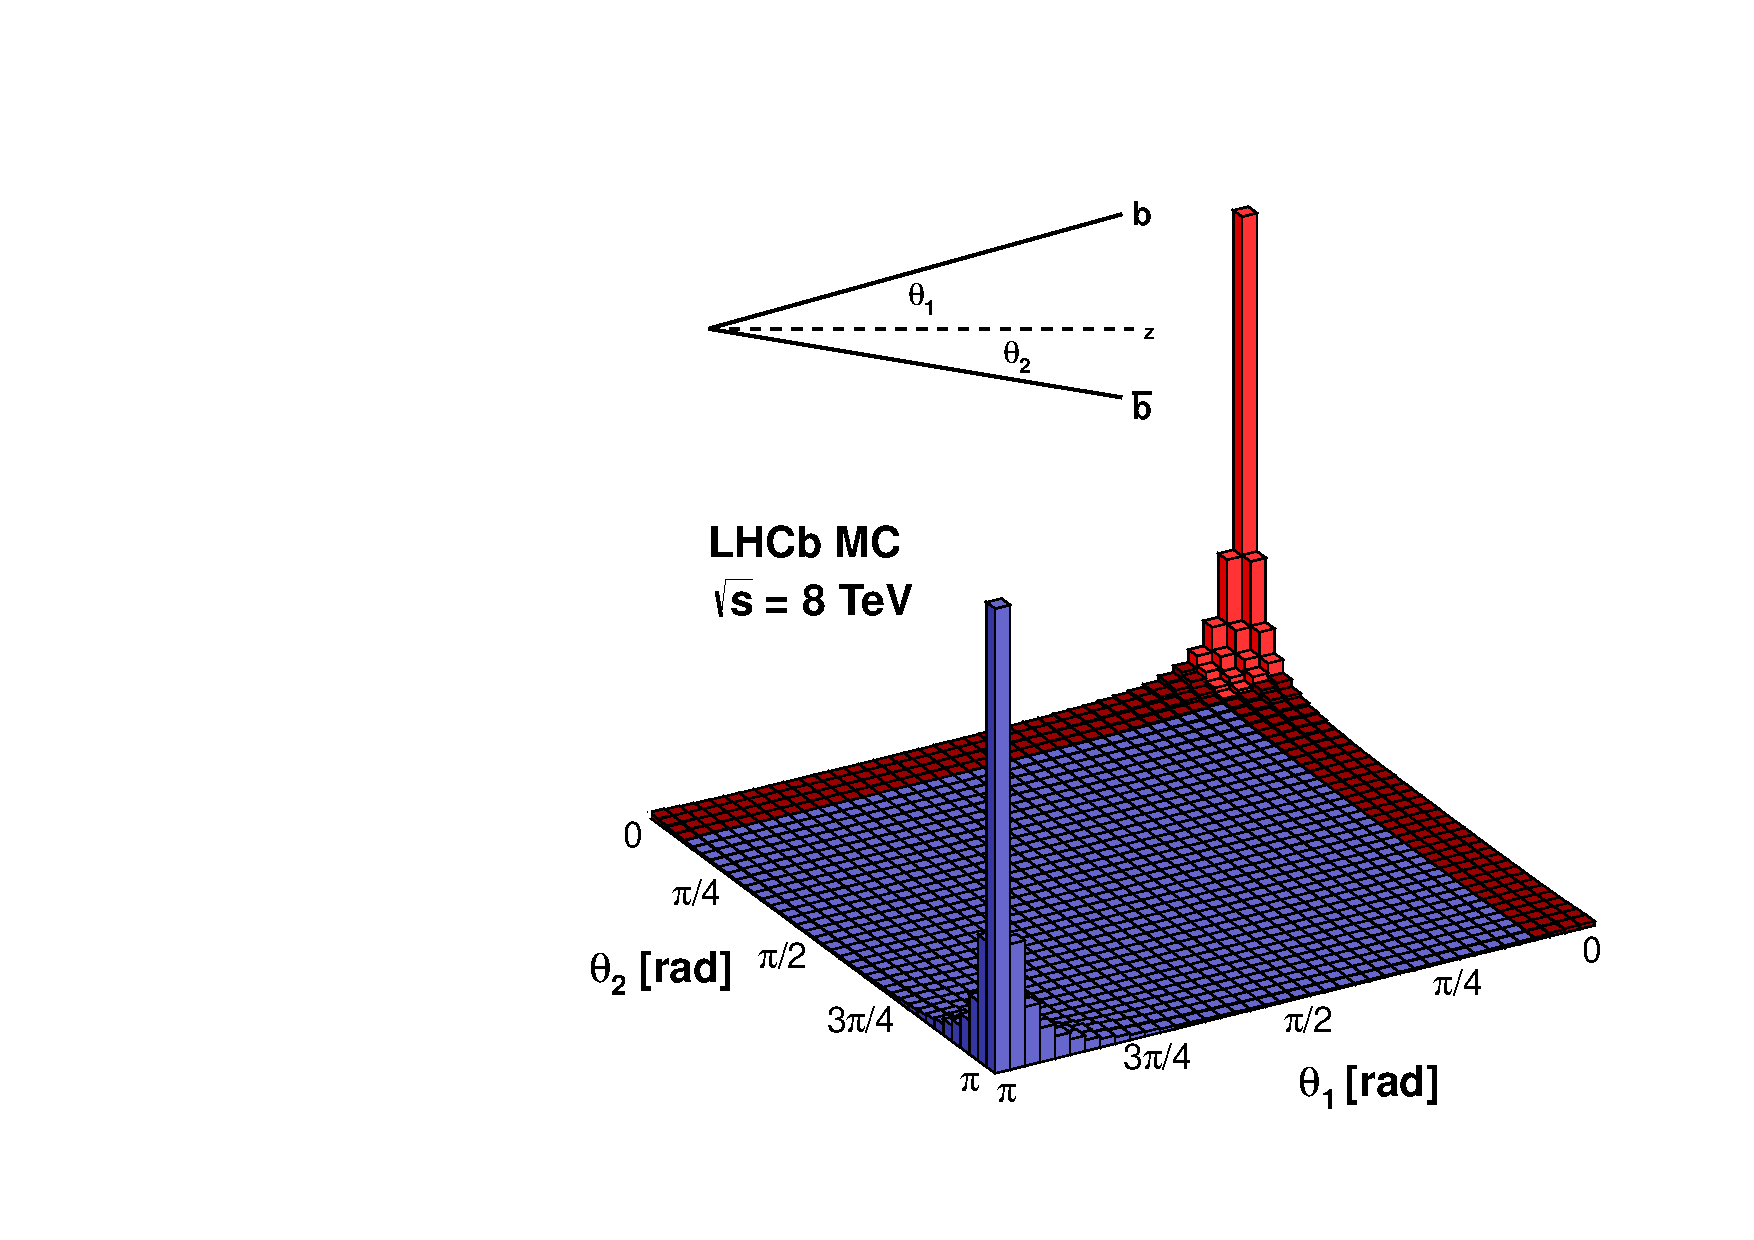
\includegraphics[width=0.6\textwidth]{figs/Detector/bb_acceptance.pdf}
    \caption{The angular distribution of \bquark\bquarkbar pair production in simulated \proton \proton collisions at a centre-of-mass energy of 8\,TeV~\cite{bbproduction}. The acceptance of \lhcb is highlighted in red.}
    \label{fig:Dec_bb_production}   
\end{figure}
% %%%%%%%%%%%%%%%%%%%%%%%%%%%%%%%%%%%%%%%%%%%%%%%%%%%%%%%%%%


Running along the centre of the detector is the \lhcb beampipe. The primary role is to separate the inner vacuum chamber from the rest of the cavern, allowing the beams to circulate in vacuum. Within the \lhcb tracker the beampipe is made of beryllium, with smaller sections made out of aluminium alloys or stainless steel. Although beryllium is a highly toxic and fragile material it has a long radiation length, allowing the incident particles to traverse the pipe walls with minimal interactions.  


\subsection{Magnet}

The \lhcb detector contains a warm dipole magnet that bends the trajectories of charged particles, allowing measurements of the particles' momentum. The magnet has two saddle-shaped coils inside a square yoke that generate an average integrated magnetic field of 4\,Tm.  
The magnetic field is aligned along the $y$-axis, bending the charged particles in the horizontal plane. The polarity of the magnet is routinely switched during data taking. This helps to understand and cancel systematic effects that may affect measurements of \CP asymmetries. The two magnet polarities are referred to \MagDown and \MagUp, corresponding to a field in the negative and positive $y$-axis direction respectively.   

A schematic of the magnet is shown in Fig.~\ref{fig:Dec_magnet}, along with the strength of the magnetic field as a function of the $z$-axis position. Both magnet polarities are represented in this figure. 


%%%%%%%%%%%%%%%%%%%%%%%%%%%%%%%%%%%%%%%%%%%%%%%%%%%%%%%%%%
\begin{figure}[!h]
    \centering
    \begin{subfigure}[t]{0.4\textwidth}
        \centering
        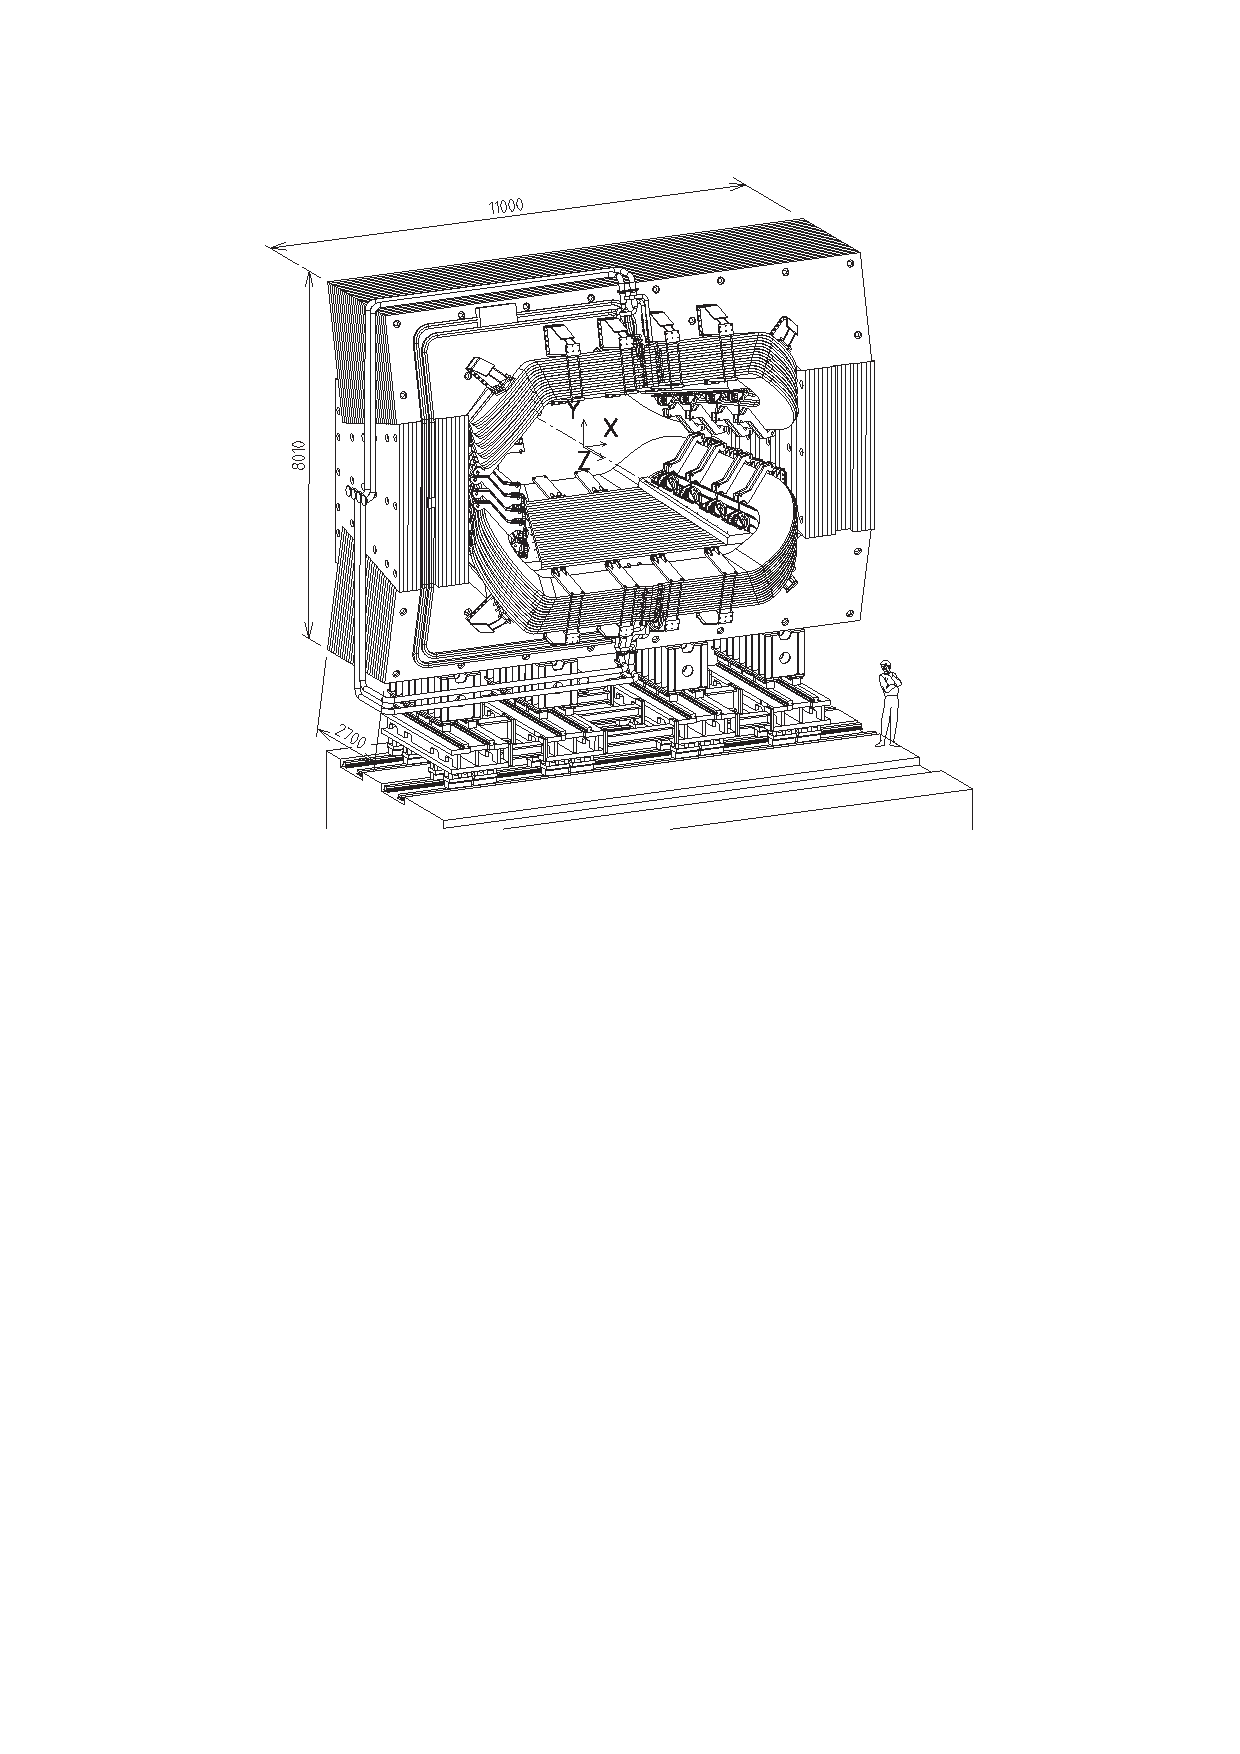
\includegraphics[width=1.0\textwidth]{figs/Detector/magnet_schematic.pdf}
    \end{subfigure}
    \begin{subfigure}[t]{0.4\textwidth}
        \centering
        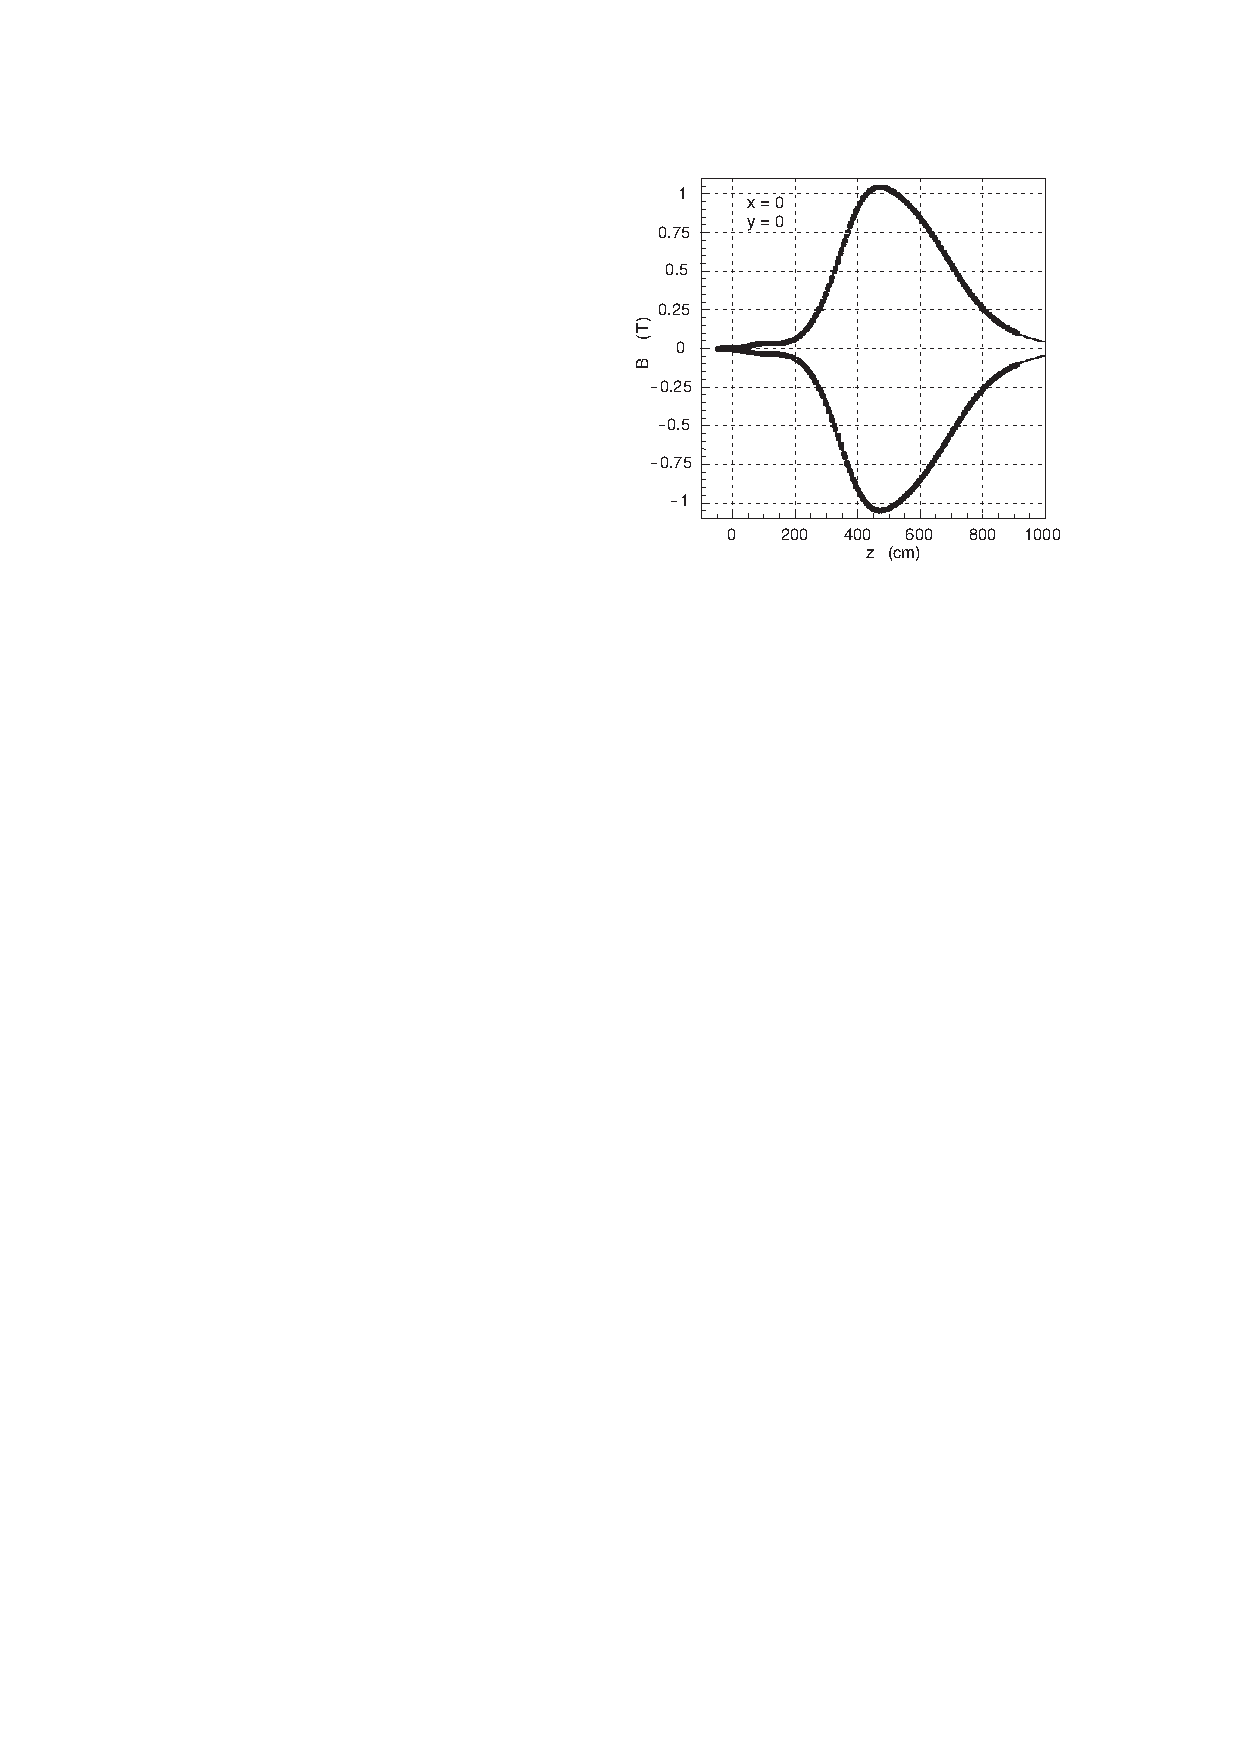
\includegraphics[width=1.0\textwidth]{figs/Detector/magnet_B_field.pdf}
    \end{subfigure}
    \caption{Schematic of the \lhcb dipole magnet (left) and the magnetic field strength along the $z$-axis (right) from Ref.~\cite{Alves:2008zz}.}
    \label{fig:Dec_magnet}   
\end{figure}
%%%%%%%%%%%%%%%%%%%%%%%%%%%%%%%%%%%%%%%%%%%%%%%%%%%%%%%%%%


\subsection{Vertex Locator}

The first sub-detector to make measurements of the particles produced in proton-proton collisions is the Vertex Locator (\velo) encompassing the collision region. This sub-detector makes precise measurements of the track positions of charged particles as they emanate out of the collisions. A high level of precision is required to identify the secondary vertices characteristic of \bquark- and \cquark-hadron decays. These secondary vertices are typically displaced from the interaction position as a result of the long lifetimes associated to these heavy-flavour hadrons. This is achieved by measuring the track coordinates using silicon strip sensors placed as close to the \lhc beam as safety allows. The \velo sensors are semicircular devices placed on either side of the beam. To allow the sensors to instrument the innermost region around the interaction point the two halves of the \velo can move horizontally in and out. During normal data taking this allows the sensors to be 7\mm away from the interaction point yet still be a safe distance away from the beams at injection. 

%%%%%%%%%%%%%%%%%%%%%%%%%%%%%%%%%%%%%%%%%%%%%%%%%%%%%%%%%%
\begin{figure}[!h]
    \centering   
    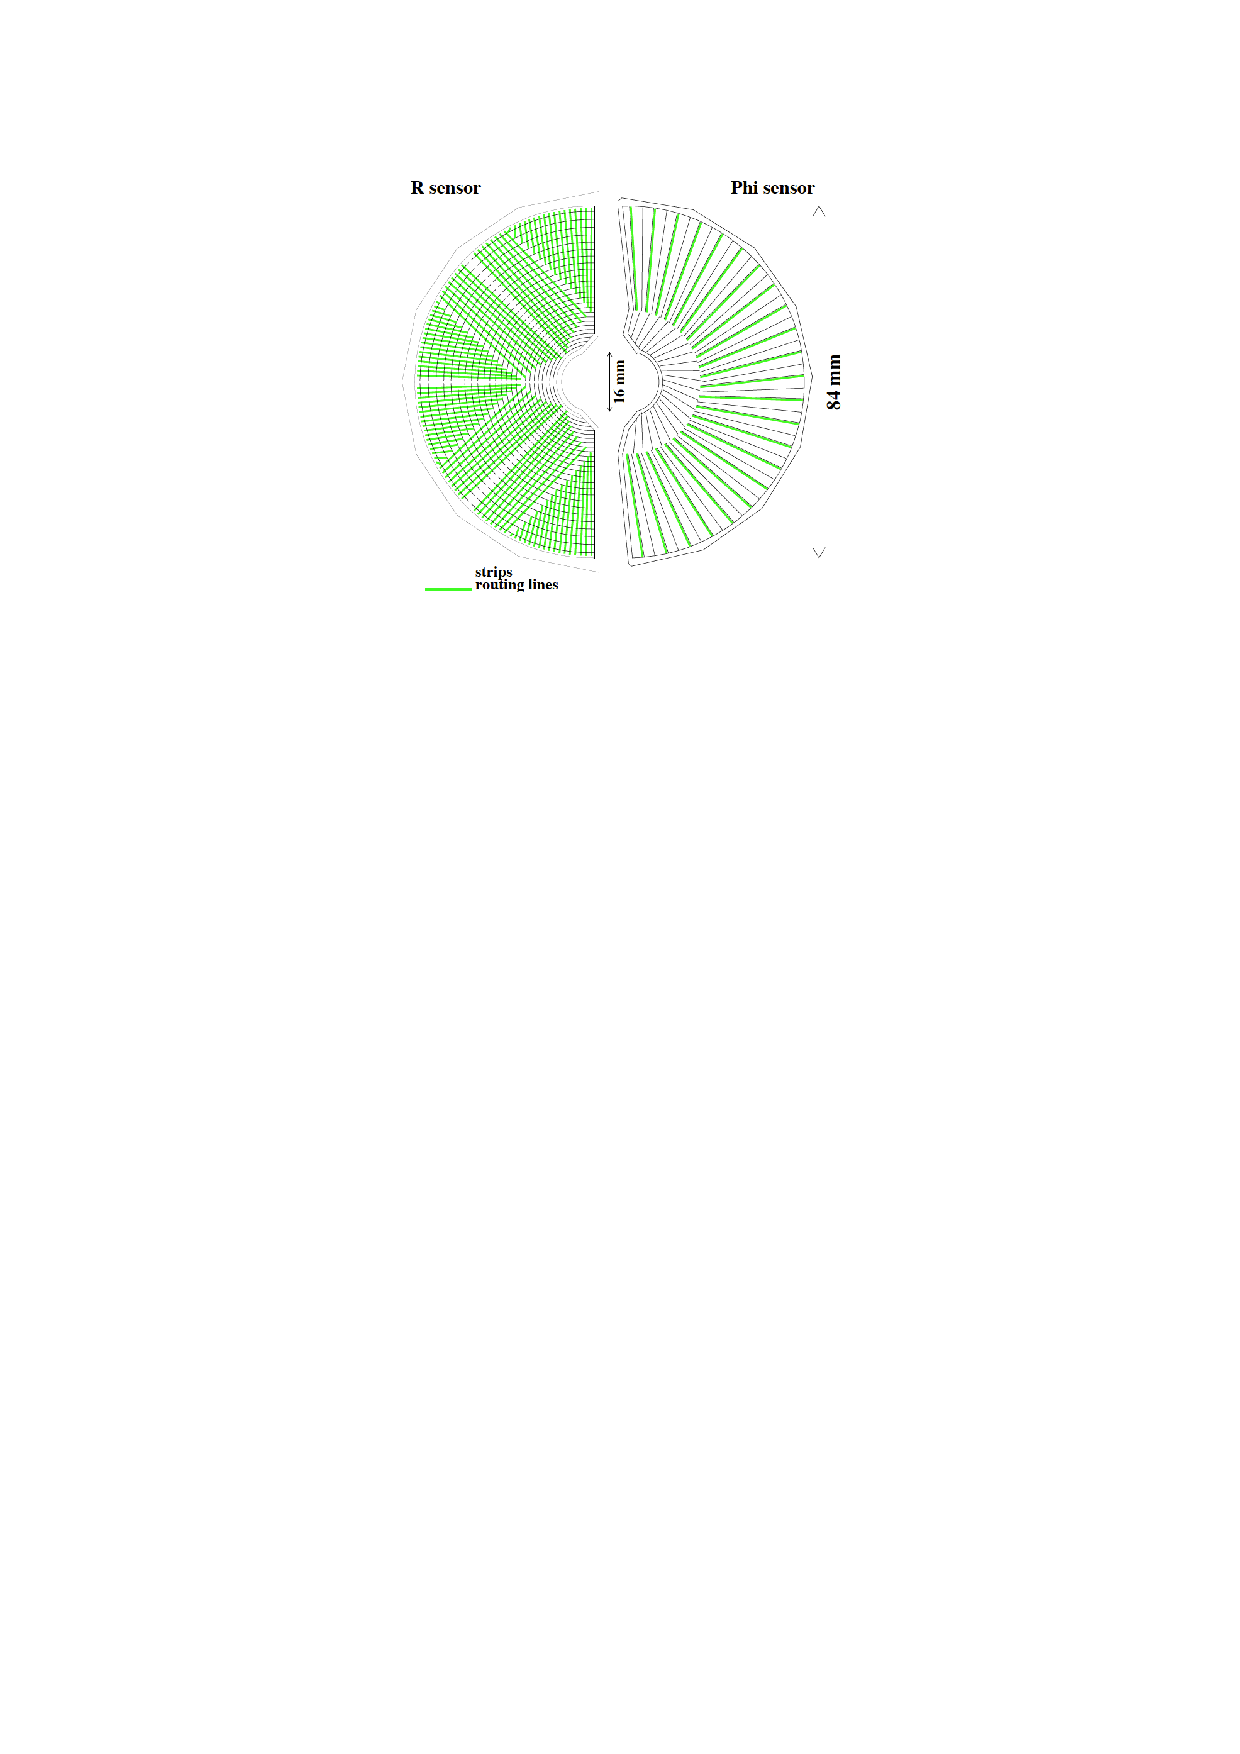
\includegraphics[width=0.4\textwidth]{figs/Detector/velo_r_phi_sensor.pdf}
    \caption{Schematic of an $r$- and $\phi$-sensor in the \velo sub-detector, from Ref.~\cite{LHCb-DP-2014-001}.}
    \label{fig:Dec_r_phi_sensor}   
\end{figure}
%%%%%%%%%%%%%%%%%%%%%%%%%%%%%%%%%%%%%%%%%%%%%%%%%%%%%%%%%%

The sensors are grouped into pairs and built into a module. Each of the 21 modules has, on opposing sides, sensors for measuring the radial and azimuthal coordinates of the tracks, referred to as $r$- and $\phi$-sensors respectively. A schematic of the two sensor types is shown in Fig.~\ref{fig:Dec_r_phi_sensor}, illustrating the silicon strips and readout channels. 


The \velo modules are arranged to ensure coverage of particles emerging in forward region at angles of 15--300\mrad with respect to the beam-pipe. This arrangement allows tracks within this acceptance to interact in at least three sensors as shown in Fig.~\ref{fig:Dec_velo_sensor_layout}.   
The modules extend both forward and backwards of the interaction region. Although momentum measurements are not possible for backward tracks, the vertexing of the primary interaction can benefit from this extra information. In the far backward region there are two additional modules, measuring only the radial coordinate. 
%These help to identify pile-up events in which there is more than one primary vertex. 
These were originally intended to help reduce pile-up problems but are now simply used as part of the PV measurement.

%%%%%%%%%%%%%%%%%%%%%%%%%%%%%%%%%%%%%%%%%%%%%%%%%%%%%%%%%%
\begin{figure}[!h]
    \centering
    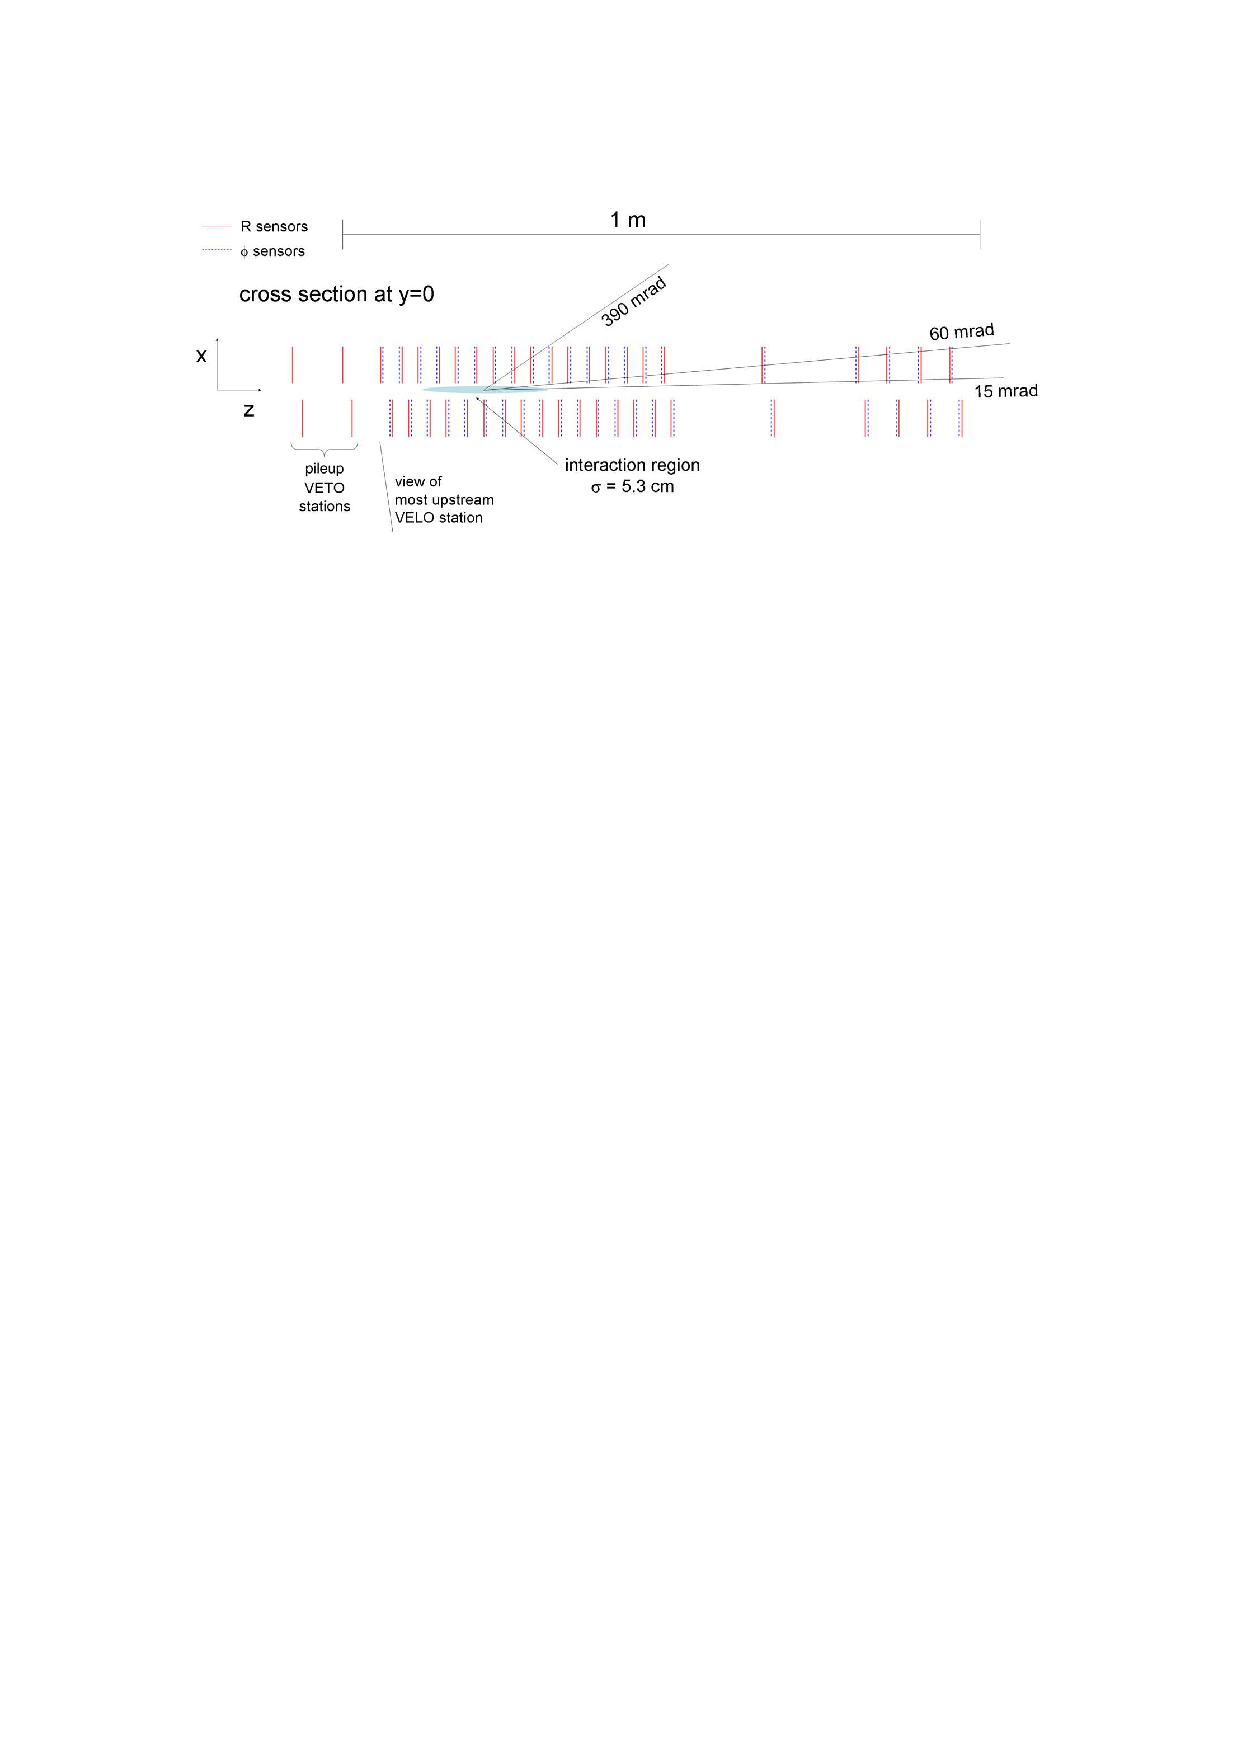
\includegraphics[width=0.8\textwidth]{figs/Detector/velo_sensor_layout.pdf}
    \caption{Schematic of the sensor layout in the \velo sub-detector, from Ref.~\cite{LHCb-DP-2014-001}.}
    \label{fig:Dec_velo_sensor_layout}   
\end{figure}
%%%%%%%%%%%%%%%%%%%%%%%%%%%%%%%%%%%%%%%%%%%%%%%%%%%%%%%%%%

The \velo sub-detector was constructed with the following features to withstand the harsh environment close to the \lhc beams,
\begin{description}   
\item \textbf{Radiation resistance:} the \velo modules are subjected to extreme and varying amounts of radiation. The detector is designed to with stand three years of nominal \lhc running, using a radiation tolerant silicon. Additionally, the \velo modules are cooled to remove the heat created from the interactions. The sensors are maintained at a temperature between -10 and 0\degrees{C} with 24\,W of heat removed from each module.  
\item \textbf{Radio-frequency (RF) pick-up protection:} the mirror electromagnetic fields generated by the passing \lhc beams would generate large pick-up noise in the \velo detectors electronics. Therefore, a metal shield separates the module volume and the beam-pipe vacuum. The RF-foil is 0.3\mm thick and also serves to separate the \velo and beam-pipe vacuums. The beam vacuum has a pressure of $\sim 10^{-10}\,\text{mbar}$ whilst the \velo vacuum is limited to $\sim 10^{-6}\,\text{mbar}$ due to out-gassing.

%could cause interference in the \velo detectors electronics. Therefore, a shield is used between the modules and the beam-pipe referred to as the RF-foil. This 0.3\mm thick foil separates the \velo and beam-pipe vacuums, providing additional protection to the conditions of the beams from the \velo detector itself.
\end{description}   

The hits arising from particle interactions in the \velo sensors are extracted from the readout channels using custom analogue chips. The data is zero-suppressed and combined into clusters in Field-programmable Gate Array (FPGA) boards called the \tellone boards~\cite{HAEFELI2006494}, 


The performance of the \velo sub-detector is quantified by the track finding efficiency and the resolution of the impact parameter. 
The track finding efficiency determines the likelihood that a track will be reconstructed and is of particular importance for high multiplicity final states including those presented in this thesis. The average track finding efficiency in data taken during 2011 is found to be around 98\% as shown in Fig.~\ref{fig:Dec_velo_track_performance}. This drops to 97\% by 2016 due to radiation damage.

The impact parameter (IP) represents the distance between a track and a primary vertex at the point of closest approach. Long-lived particles, such as \Bp mesons, decay at a secondary vertex displaced from the primary collision vertex. Therefore, the decay products of these particles have a larger IP than tracks originating at the primary vertex. A precise measurement of the IP of a track allows the \Bp mesons and various background processes to be differentiated. The distribution of the $x$-component of the IP is shown as a function of the inverse transverse momentum ($1/\pt$) in Fig.~\ref{fig:Dec_velo_track_performance}.  

%%%%%%%%%%%%%%%%%%%%%%%%%%%%%%%%%%%%%%%%%%%%%%%%%%%%%%%%%%
\begin{figure}[!h]
    \centering
    \begin{subfigure}[t]{0.4\textwidth}
        \centering
        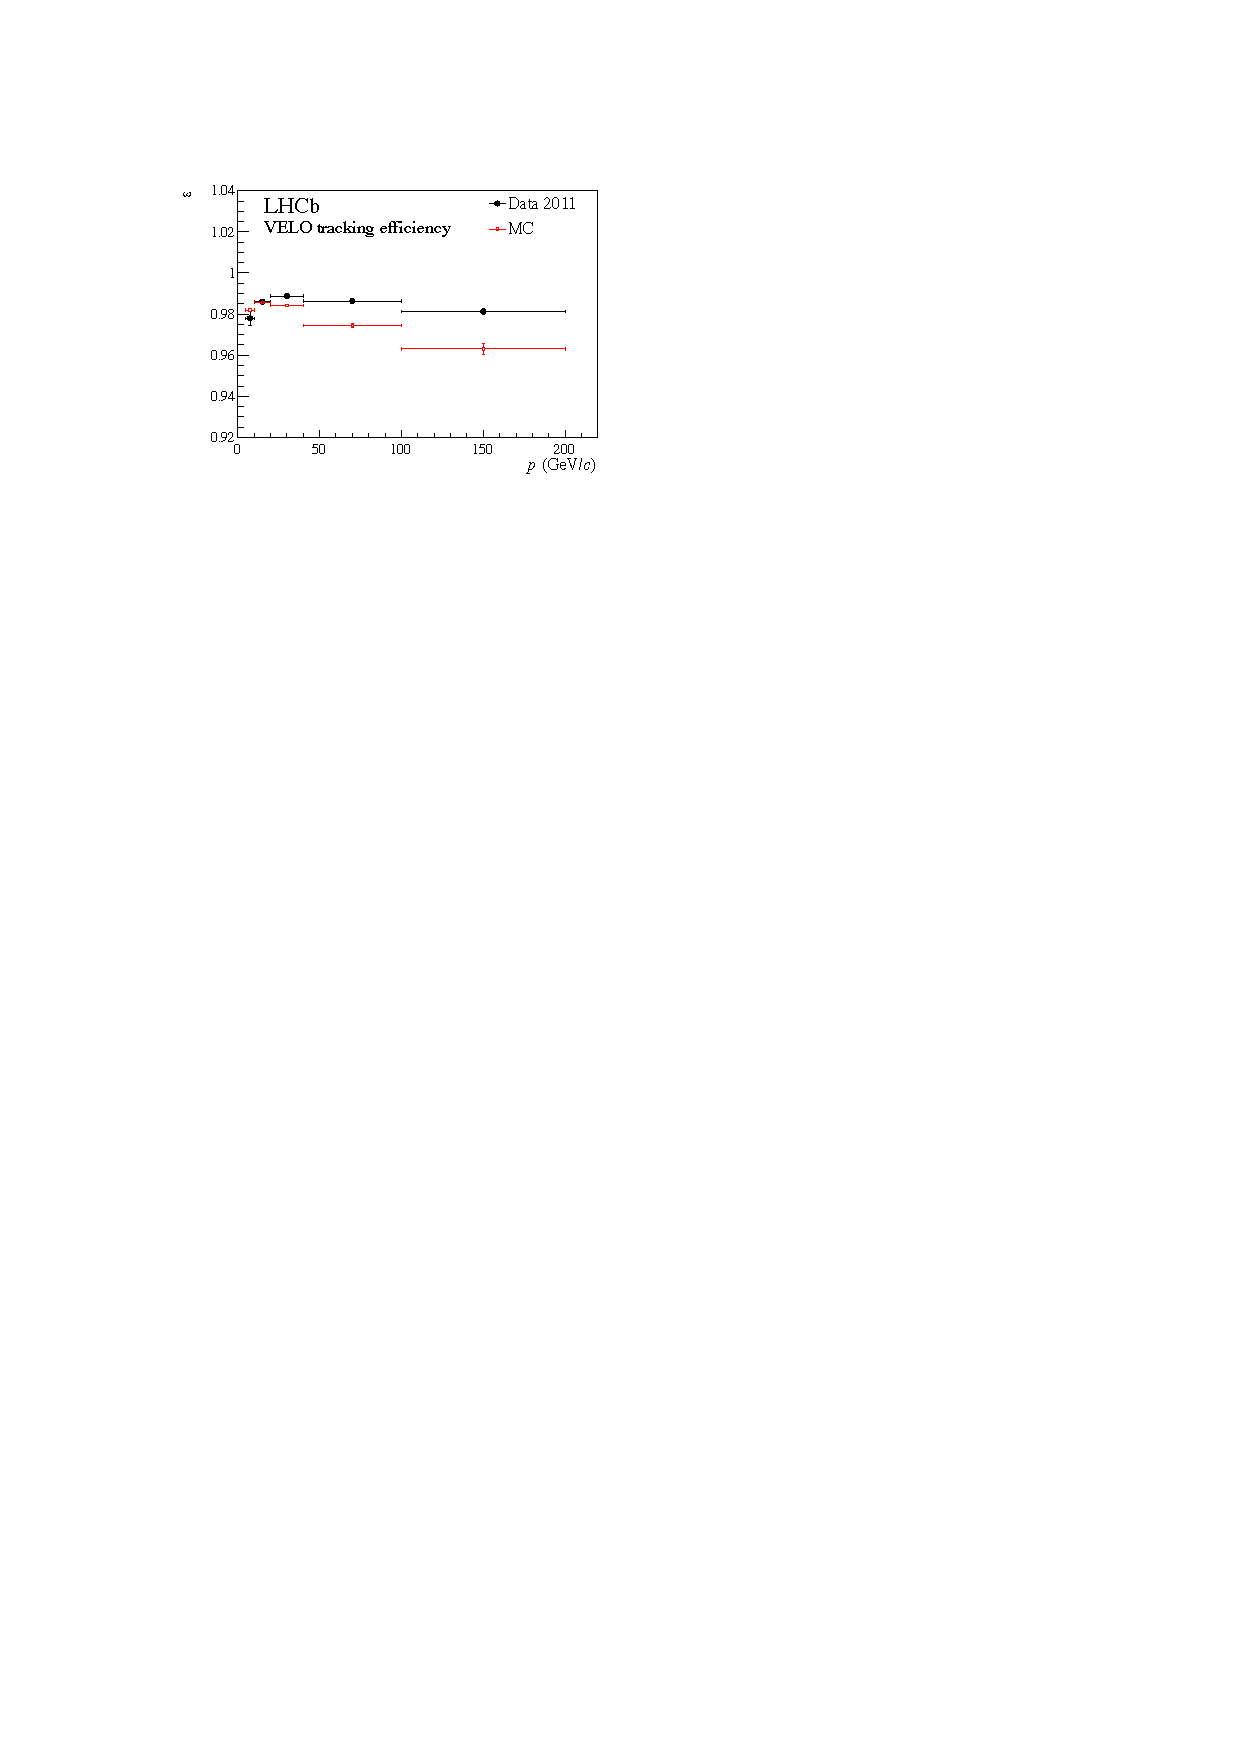
\includegraphics[width=1.0\textwidth]{figs/Detector/velo_track_eff_2011.pdf}
    \end{subfigure}
    \begin{subfigure}[t]{0.4\textwidth}
        \centering
        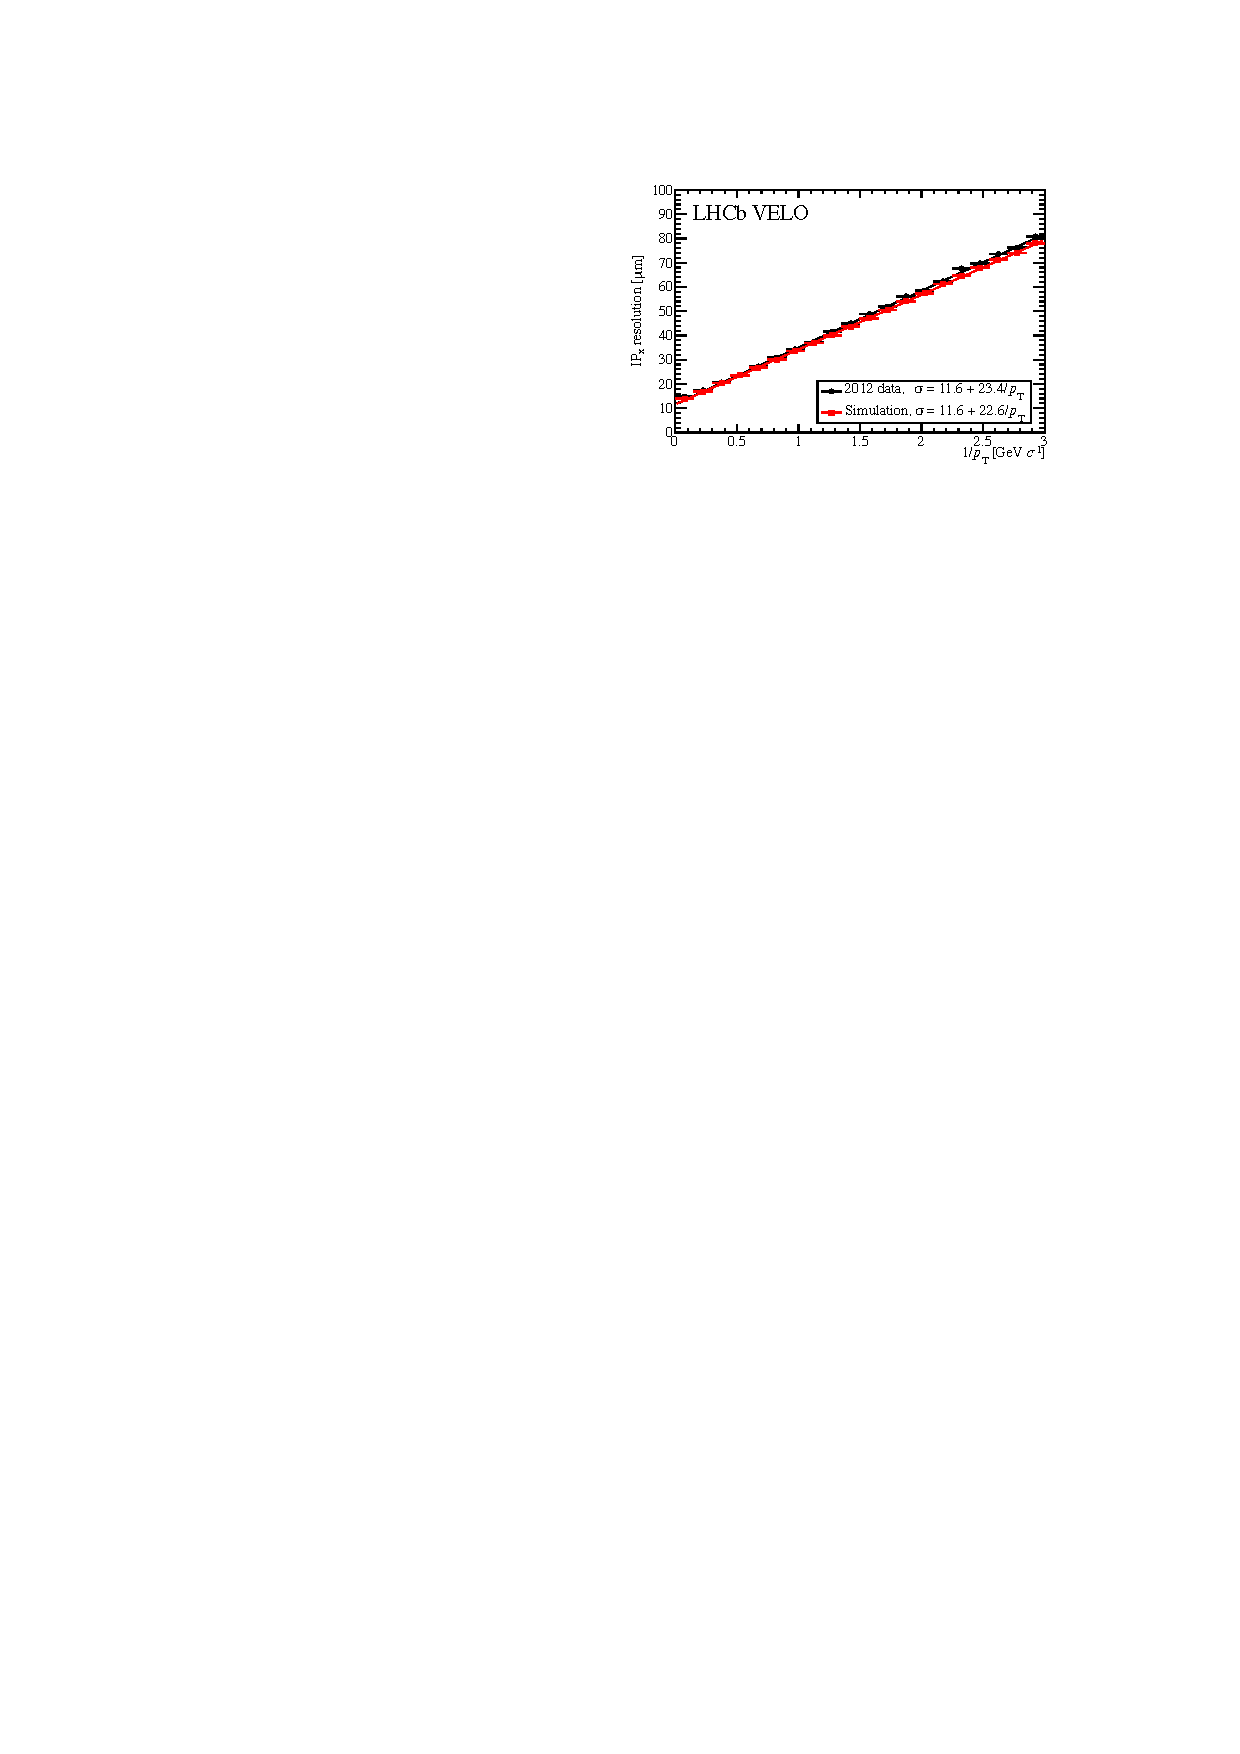
\includegraphics[width=1.0\textwidth]{figs/Detector/velo_ipx_resolution.pdf}
    \end{subfigure}
    \caption{The tracking efficiency (left) and $\text{IP}_{x}$ resolution (right) in simulation and data, from Ref.~\cite{LHCb-DP-2014-001}.}
    \label{fig:Dec_velo_track_performance}   
\end{figure}
%%%%%%%%%%%%%%%%%%%%%%%%%%%%%%%%%%%%%%%%%%%%%%%%%%%%%%%%%%

The \velo sensor performance gradually degrades with exposure to radiation. The damage to the silicon sensors is monitored over time to estimate the remaining lifetime of the sensors. In-between \lhc fills, current-voltage (IV) scans are performed on the silicon semiconductors, measuring the current leaking as a function of the bias voltage. The evolution of this current in Run I is shown in Fig.~\ref{fig:Dec_velo_run2_performance}, along with the delivered luminosity. These measurements help to predict what bias voltages will required by the end of Run II to maintain sufficient track-finding efficiency.

%%%%%%%%%%%%%%%%%%%%%%%%%%%%%%%%%%%%%%%%%%%%%%%%%%%%%%%%%%
\begin{figure}[!h]
    \centering
    \begin{subfigure}[m]{0.55\textwidth}
        \centering
        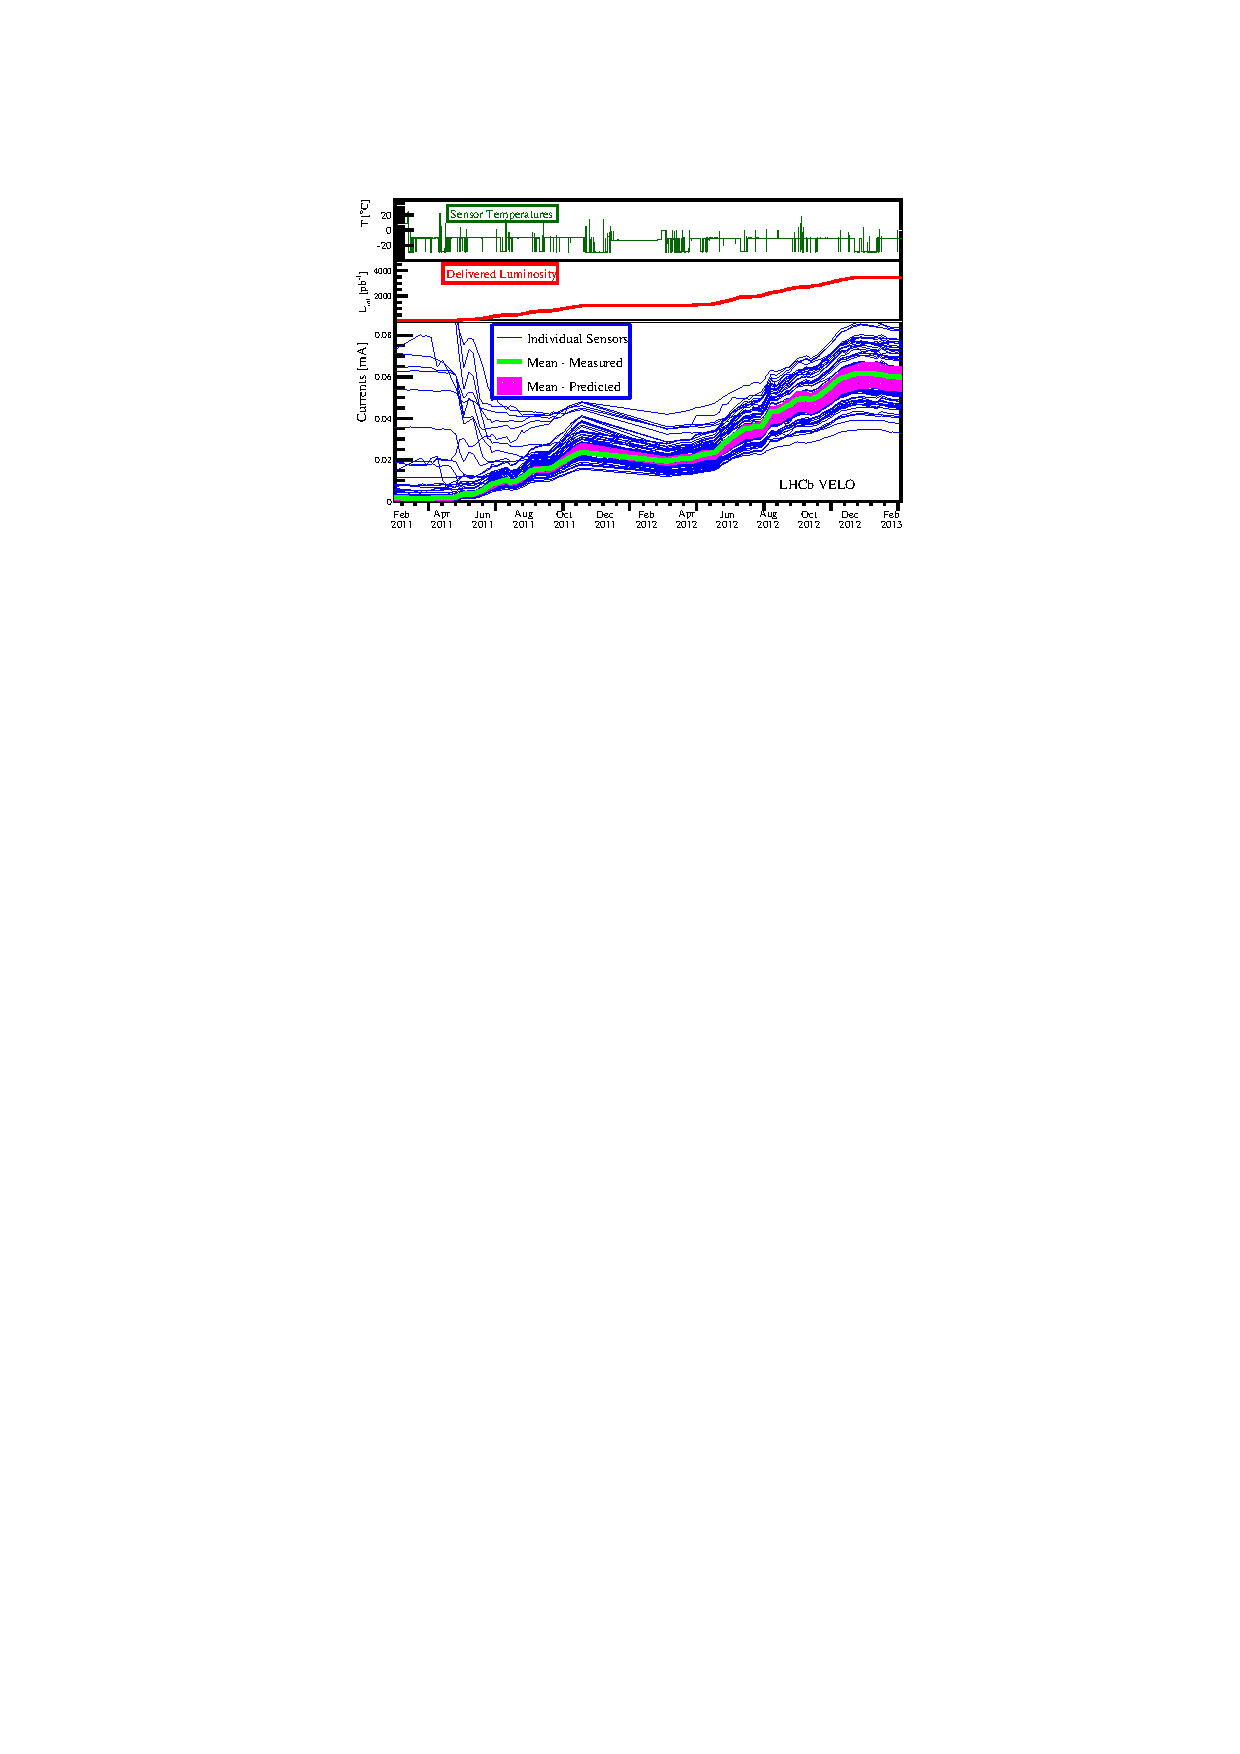
\includegraphics[width=1.0\textwidth]{figs/Detector/velo_leakage_current.pdf}
    \end{subfigure}
    \begin{subfigure}[m]{0.4\textwidth}
        \centering
        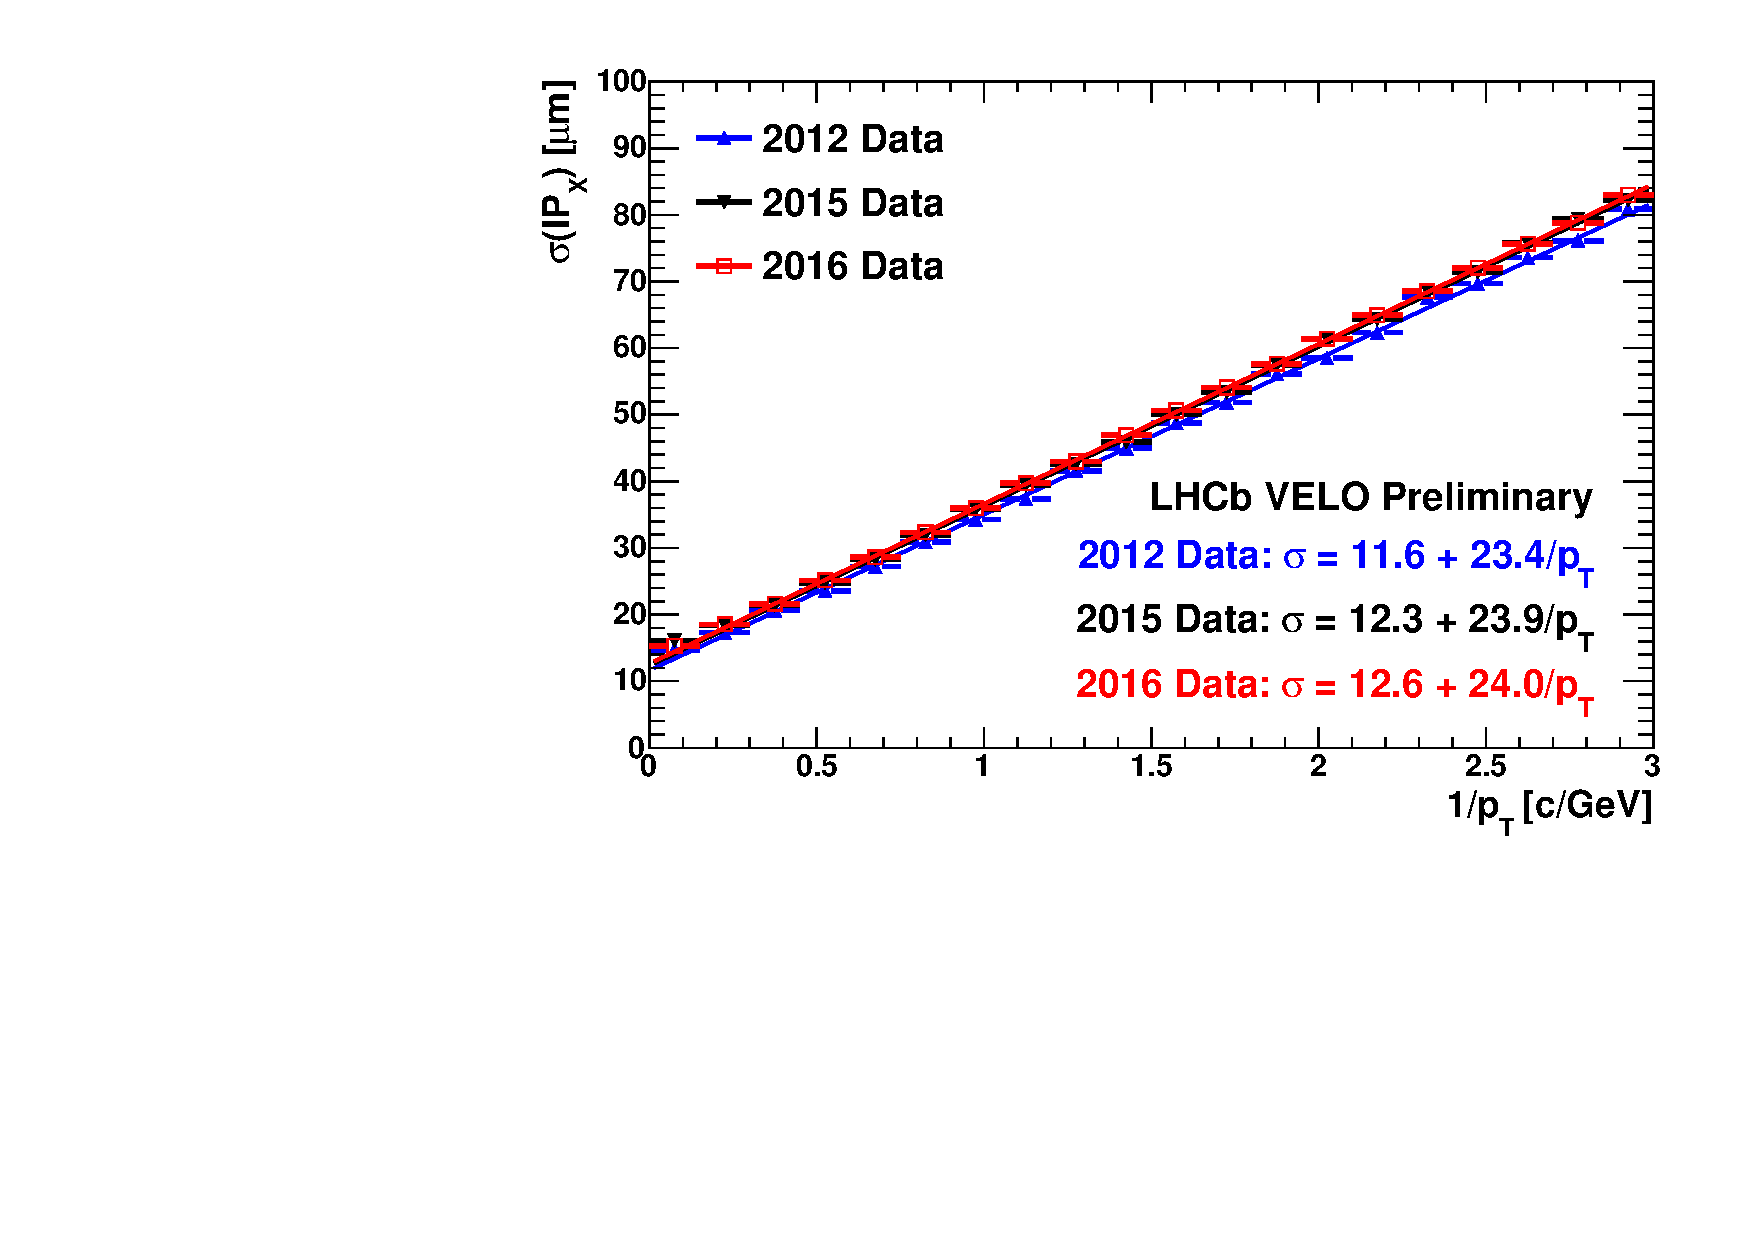
\includegraphics[width=1.0\textwidth]{figs/Detector/velo_ip_2016_2015_2012.pdf}
    \end{subfigure}
    \caption{The \velo silicon sensor's leakage current as a function of time through out Run I, from Ref.~\cite{Rinnert:2015uns} (left) and the \velo IP resolution in 2012, 2015 and 2016 data (right) . A small decrease in performance is observed between Run I and Run II.}
    \label{fig:Dec_velo_run2_performance}   
\end{figure}
%%%%%%%%%%%%%%%%%%%%%%%%%%%%%%%%%%%%%%%%%%%%%%%%%%%%%%%%%%

A comparison of the IP resolution determined using 2012, 2015 and 2016 data is also shown in Fig.~\ref{fig:Dec_velo_run2_performance}. Although the resolution is broadly similar between the three years, a slight decrease in resolution performance is present between Run I and Run II. 


% %%%%%%%%%%%%%%%%%%%%%%%%%%%%%%%%%%%%%%%%%%%%%%%%%%%%%%%%%%
% \begin{figure}[!h]
%     \centering
%     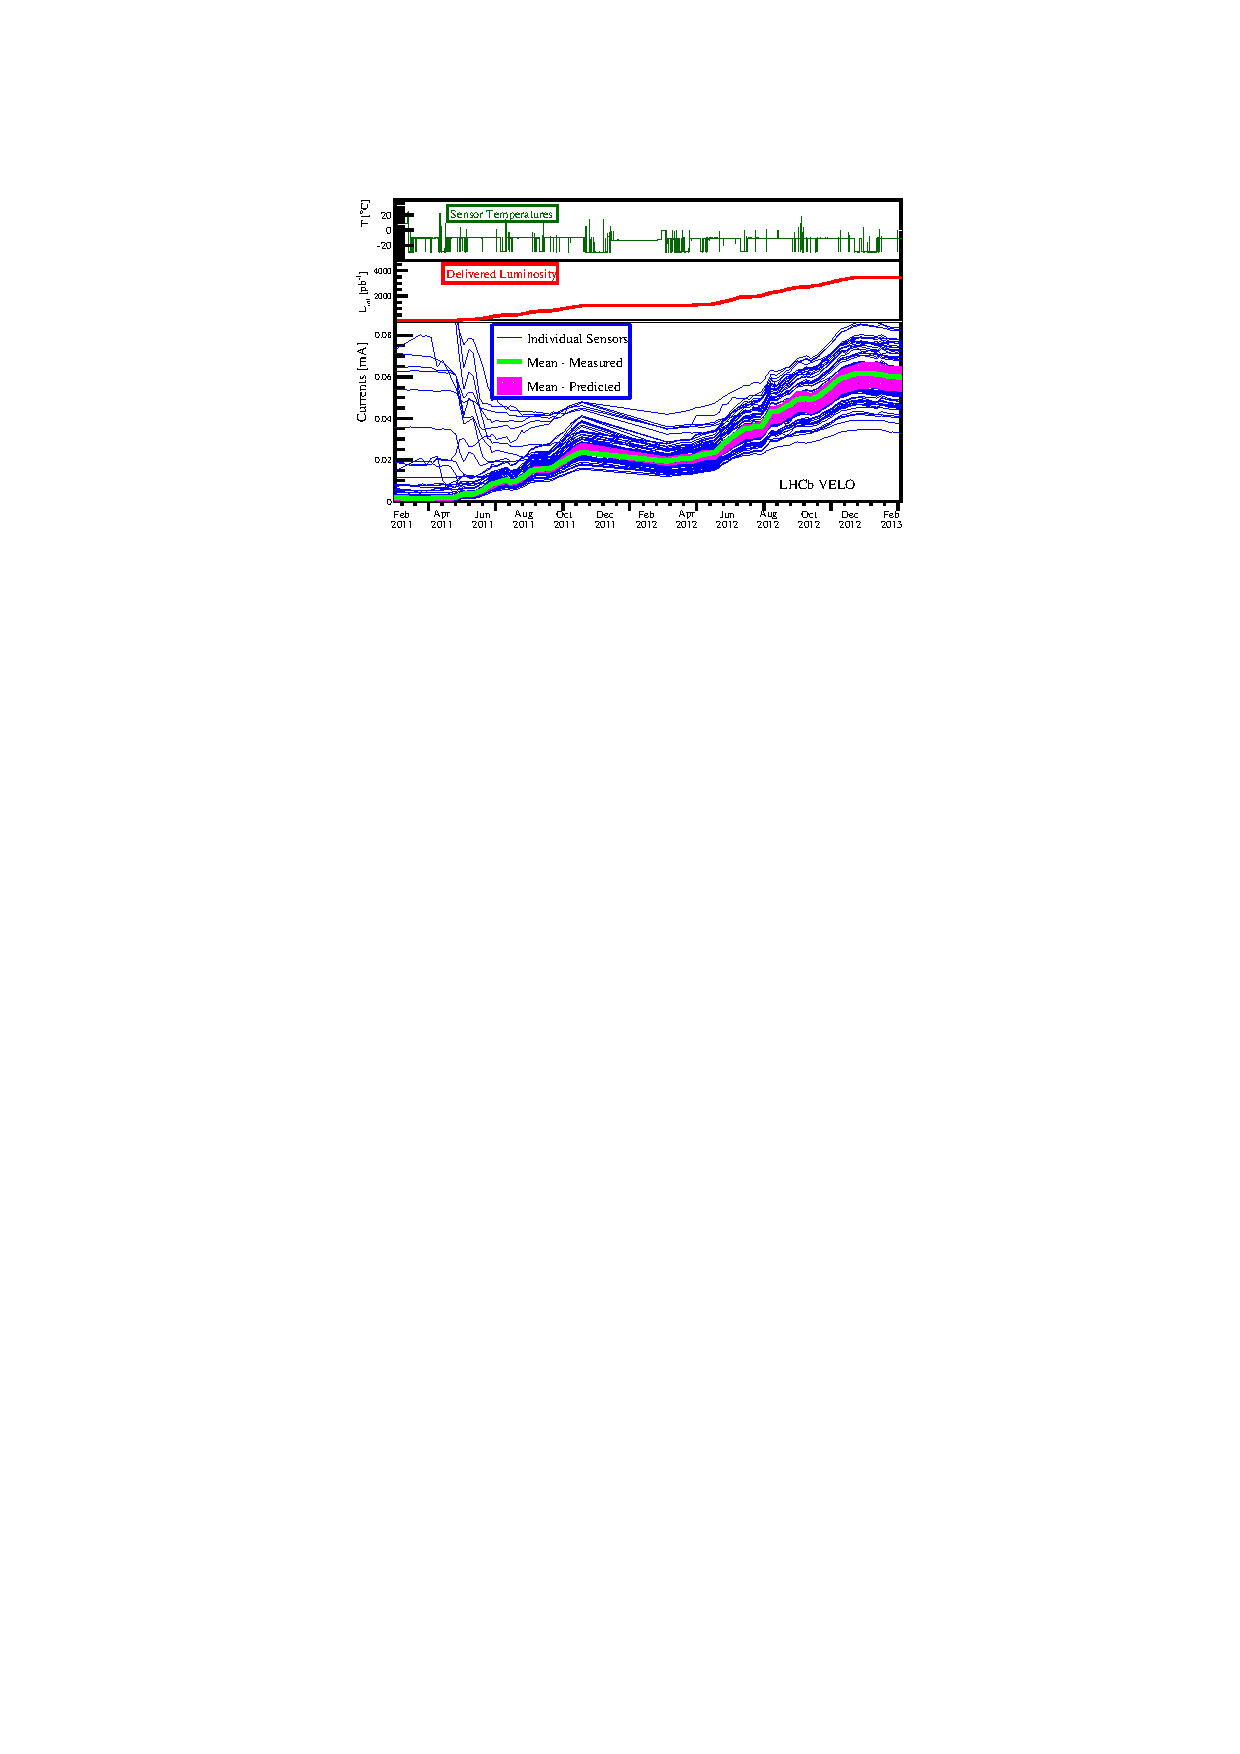
\includegraphics[width=0.6\textwidth]{figs/Detector/velo_leakage_current.pdf}
%     \caption{The \velo silicon sensor's leakage current as a function of time through out Run I, from Ref.~\cite{Rinnert:2015uns}.}
%     \label{fig:Dec_velo_leakage_current}   
% \end{figure}
% %%%%%%%%%%%%%%%%%%%%%%%%%%%%%%%%%%%%%%%%%%%%%%%%%%%%%%%%%%




% %%%%%%%%%%%%%%%%%%%%%%%%%%%%%%%%%%%%%%%%%%%%%%%%%%%%%%%%%%
% \begin{figure}[!h]
%     \centering
%     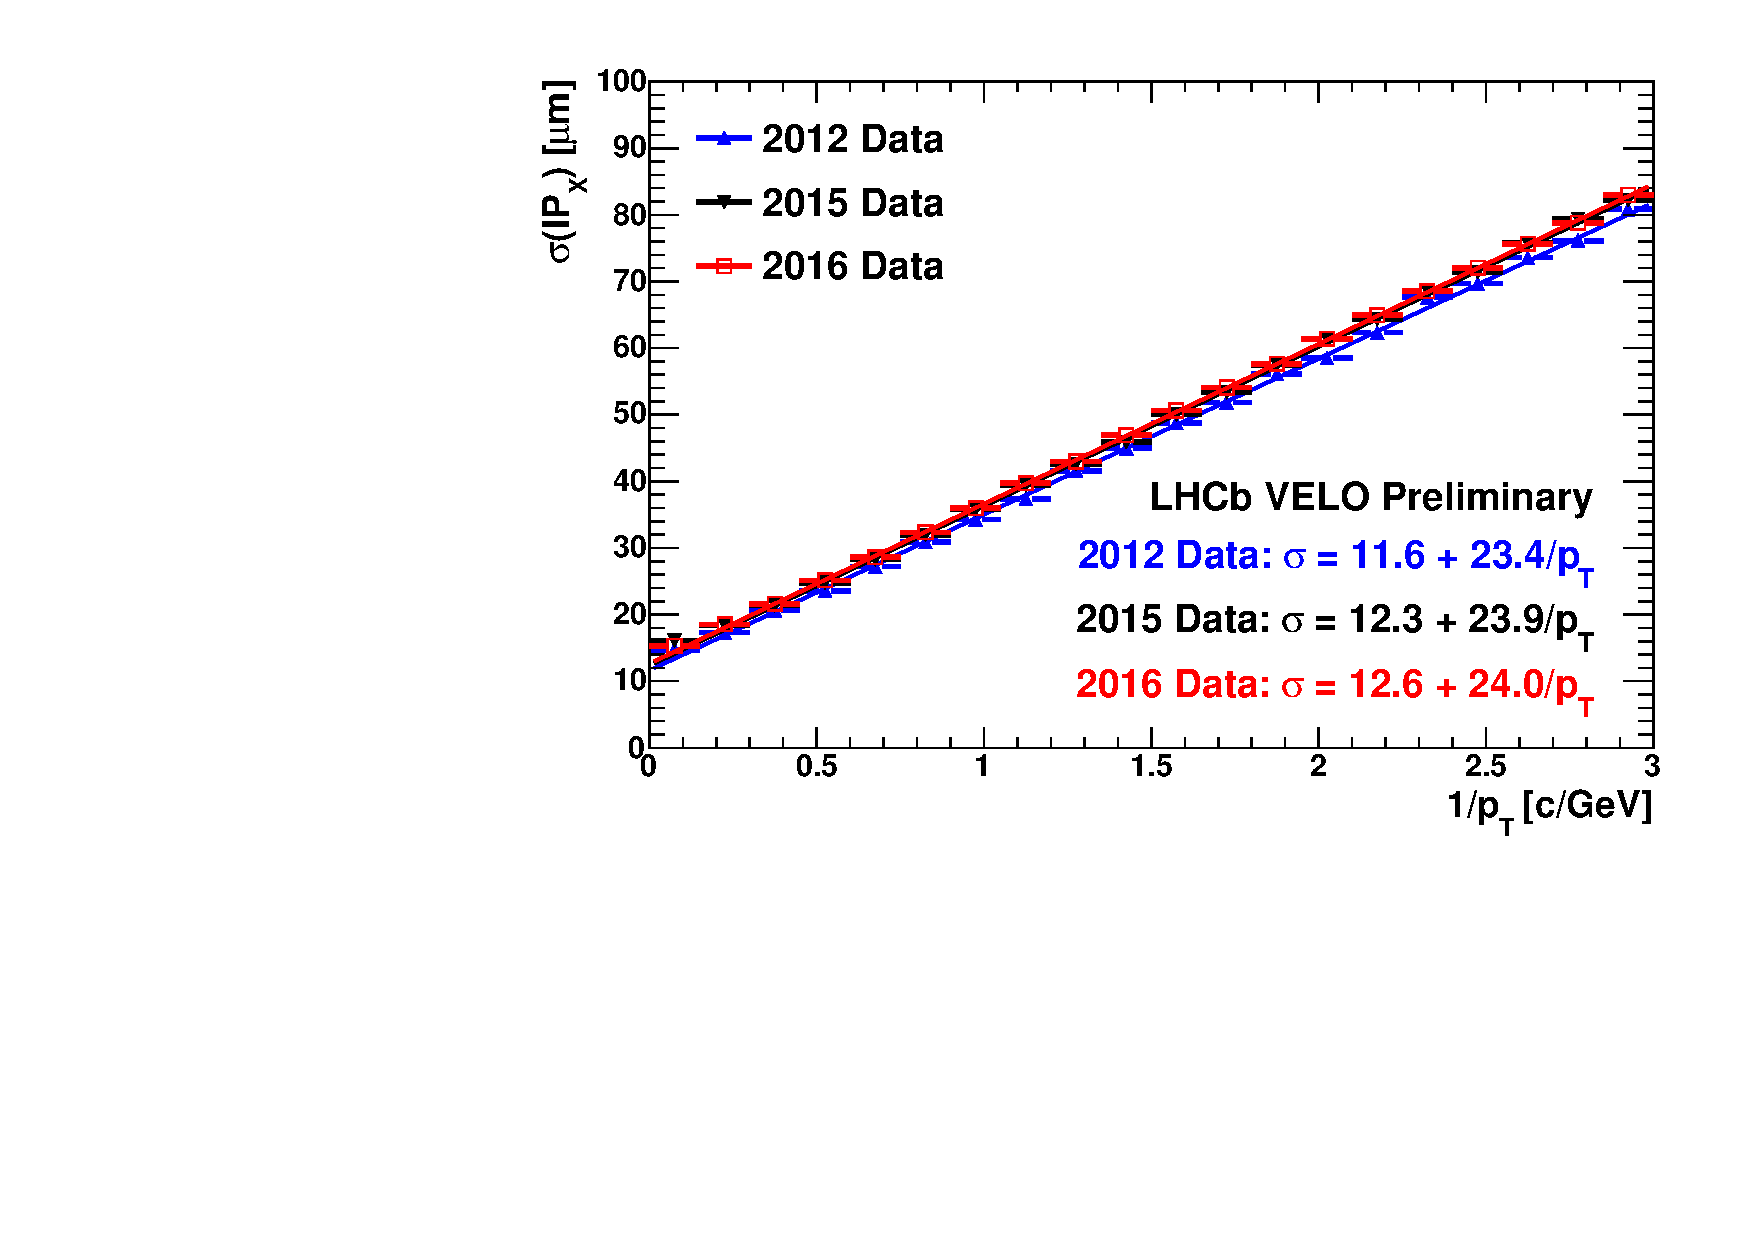
\includegraphics[width=0.4\textwidth]{figs/Detector/velo_ip_2016_2015_2012.pdf}
%     \caption{The \velo IP resolution in 2012, 2015 and 2016 data. A small decrease in performance is observed between Run I and Run II.}
%     \label{fig:Dec_velo_run1_run2_comparison}   
% \end{figure}
% %%%%%%%%%%%%%%%%%%%%%%%%%%%%%%%%%%%%%%%%%%%%%%%%%%%%%%%%%%



\subsection{Silicon Tracker}

In addition to the \velo, there are two more sub-detectors that utilise silicon sensors in order to determine tracking information. These are collectively referred to as the Silicon Tracker (\st), which is made up of two trackers; the Tracker Turicensis (\ttracker) and Inner Tracker (\intr). The \ttracker is located before the dipole magnet, whereas the \intr is positioned after, as show in Fig.~\ref{fig:Dec_lhcb_Schematic}. Although these two detectors are spatially separated, their common silicon mircostrip sensors and electronics warrant considering them together.

The silicon sensors are made up of single-sided $p^{+}$-on-$n$ sensors. The hits are read out via chips at the end of each module. These chips are the same custom analogue chips used in the \velo sub-detector. The signals pass into digitisers and then through optical fibres into \tellone boards that perform clustering algorithms.
Both sub-detectors are cooled to 5\degrees{C} and their sealed containers flushed with nitrogen gas to prevent condensation.



\subsubsection{Tracker Turicensis}

The \ttracker is positioned before the dipole magnet and covers the entire \lhcb acceptance, standing 130\cm tall and 150\cm wide.
It is made up of four layers orientated at angles to one another. The first and fourth layers are parallel, with the second and third at angles -5\degrees and +5\degrees to these respectively. The first and second are separated from the third and fourth by 27\cm along the beam axis. The layout of the silicon modules in the \ttracker is shown in Fig.~\ref{fig:Dec_tt_scematic}. The sensors are grouped into \emph{half-modules} that span half of the vertical height of the sub-detector. These are made up of seven silicon sensors and a readout hybrid outside of the \lhcb acceptance.

The \emph{half-modules} are arranged to prevent any gaps in the instrumentation. The adjacent \emph{half-modules} are offset by 1\cm along the beam axis, allowing the modules to overlap by a few millimetres in the $x$-axis. 


%%%%%%%%%%%%%%%%%%%%%%%%%%%%%%%%%%%%%%%%%%%%%%%%%%%%%%%%%%
\begin{figure}[!h]
    \centering
    \begin{subfigure}[m]{0.49\textwidth}
        \centering
        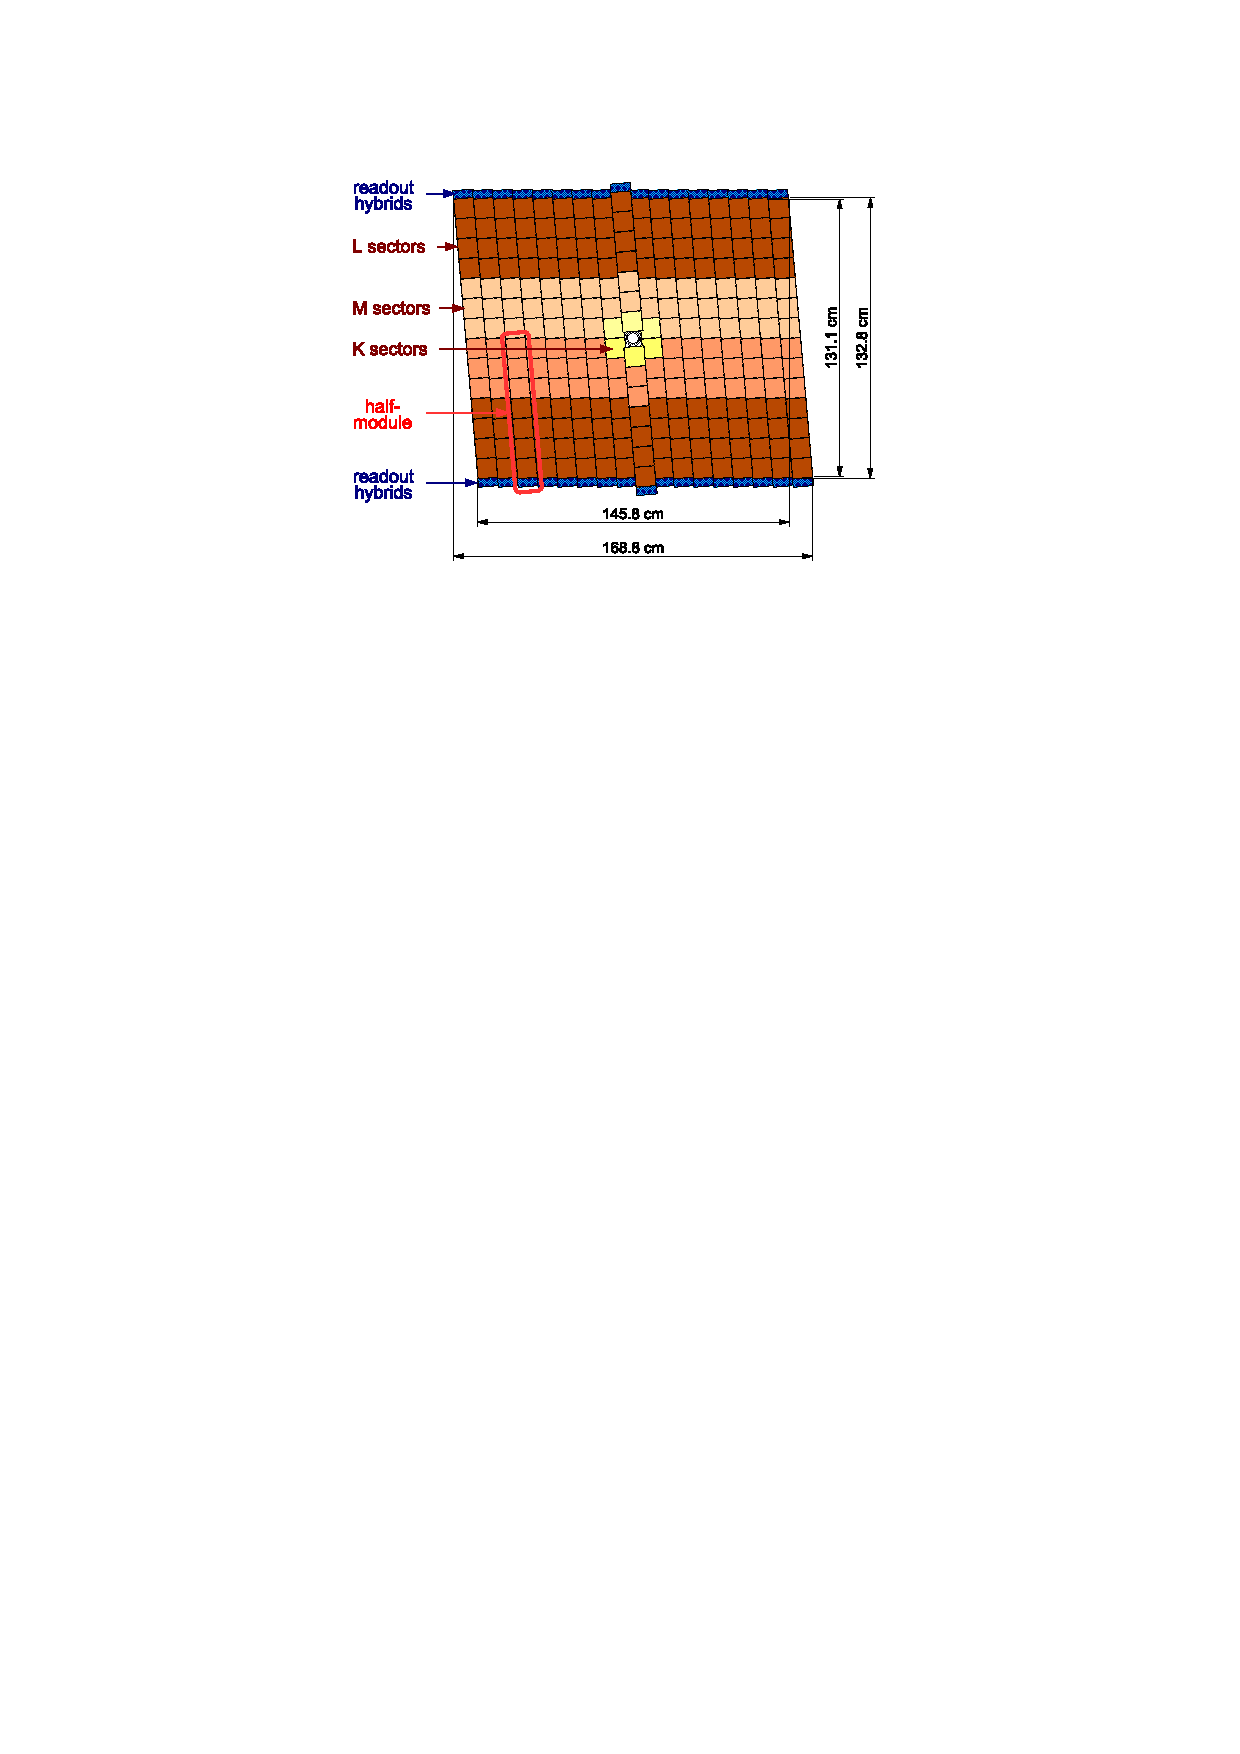
\includegraphics[width=1.0\textwidth]{figs/Detector/tt_layout.pdf}
    \end{subfigure}
    \begin{subfigure}[m]{0.49\textwidth}
        \centering
        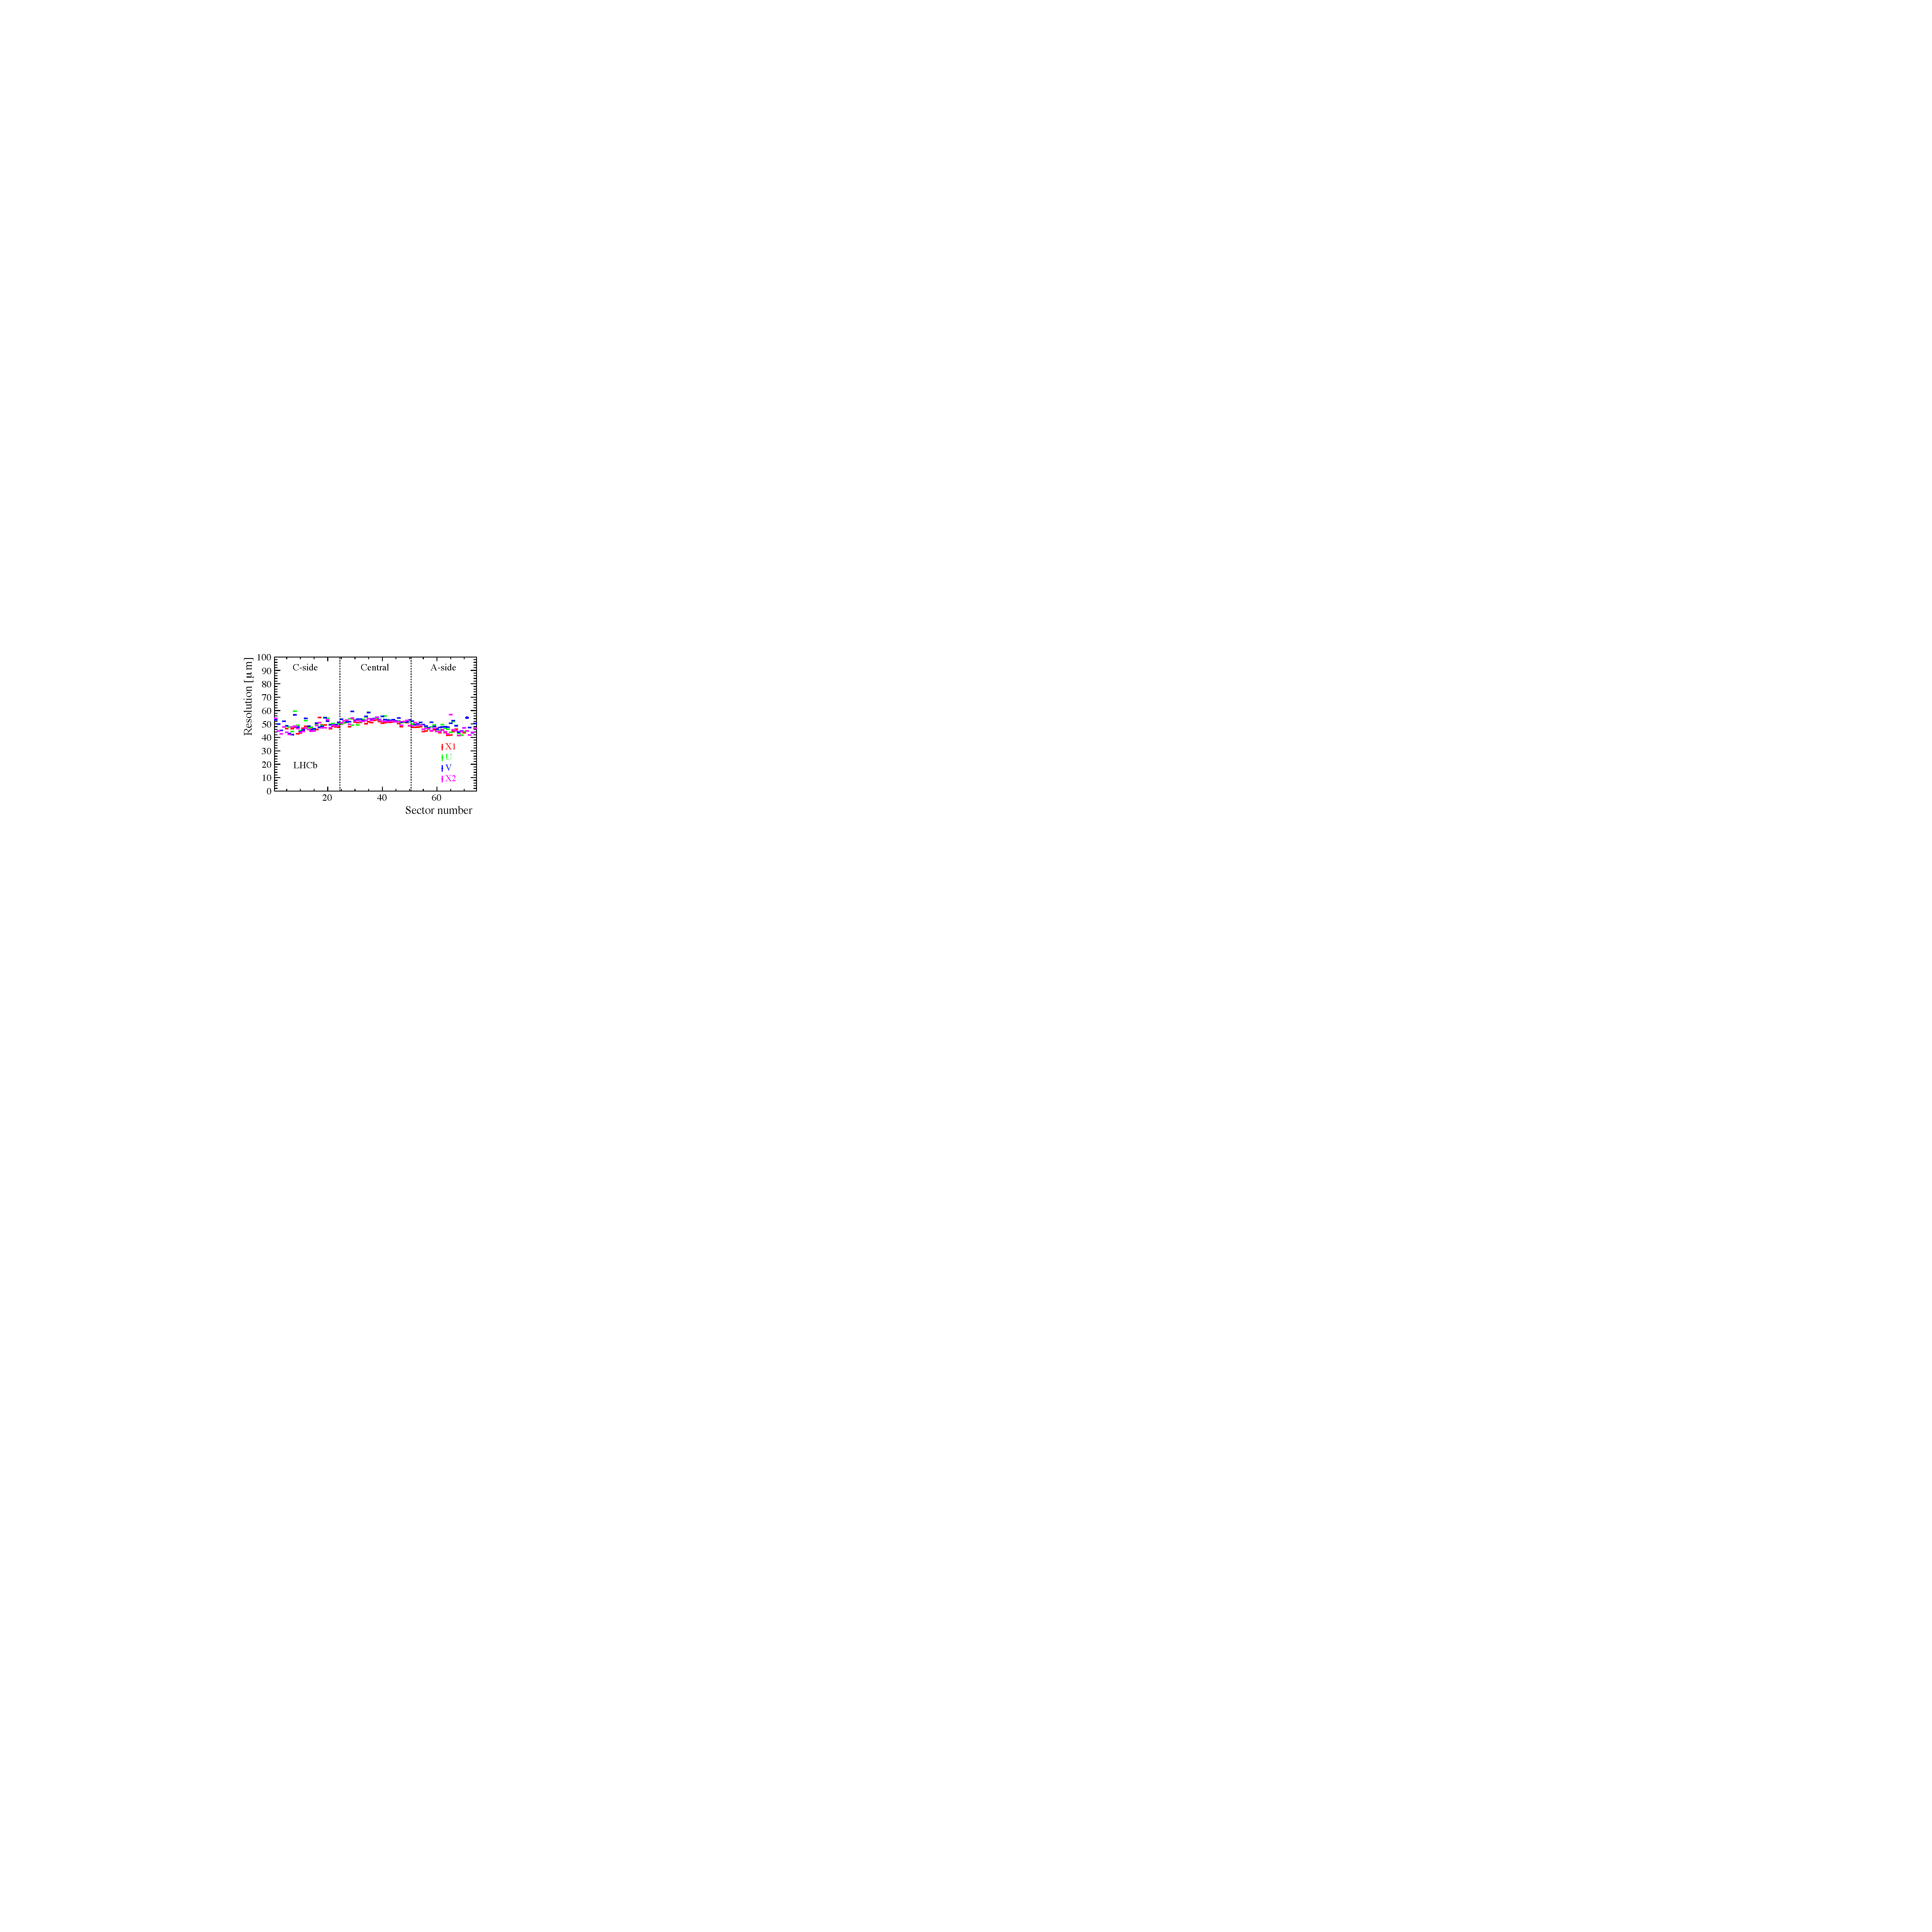
\includegraphics[width=1.0\textwidth]{figs/Detector/tt_resolution.pdf}
    \end{subfigure}
    \caption{Schematic of the third layer (labelled V) of the \ttracker sub-detector (left), from Ref.~\cite{Alves:2008zz} and the \ttracker resolution by sector number in Run I data (right), from Ref.~\cite{LHCb-DP-2014-002}.}
    \label{fig:Dec_tt_scematic}   
\end{figure}
%%%%%%%%%%%%%%%%%%%%%%%%%%%%%%%%%%%%%%%%%%%%%%%%%%%%%%%%%%


The resolution achieved by the \ttracker is shown in Fig.~\ref{fig:Dec_tt_scematic}, split into different sectors and shown separately for the four layers (labelled X1, U , V and X2). The resolution is consistent between the different layers and varies between 40--60\mum; the worst values in the central regions closest to the beam-pipe. In this region the tracks have small angles with respect to the $z$-axis leading to less charge-sharing between strips.


\subsubsection{Inner Tracker}

The \intr is located after the dipole magnet and is arranged in three tracking stations. As the name implies, it covers only the inner region of the acceptance ($3.5 < \eta < 5.0$ in the non-bending plane), measuring 140\cm wide and 40\cm tall, where the particle flux is highest. The rest of the area is covered by the larger Outer Tracker. Similar to the \ttracker, the \intr is made up of four layers positioned at slight angles to one another to maximise the precision in the bending plane. However, as shown in Fig.~\ref{fig:Dec_lhcb_Schematic}, there are three separate \intr stations, each containing four layers.
These stations are constructed as of four boxes distributed around the beam-pipe in a cross shape, as shown in Fig.~\ref{fig:Dec_it_scematic}. 



%%%%%%%%%%%%%%%%%%%%%%%%%%%%%%%%%%%%%%%%%%%%%%%%%%%%%%%%%%
\begin{figure}[!h]
    \centering
    \begin{subfigure}[m]{0.49\textwidth}
        \centering
        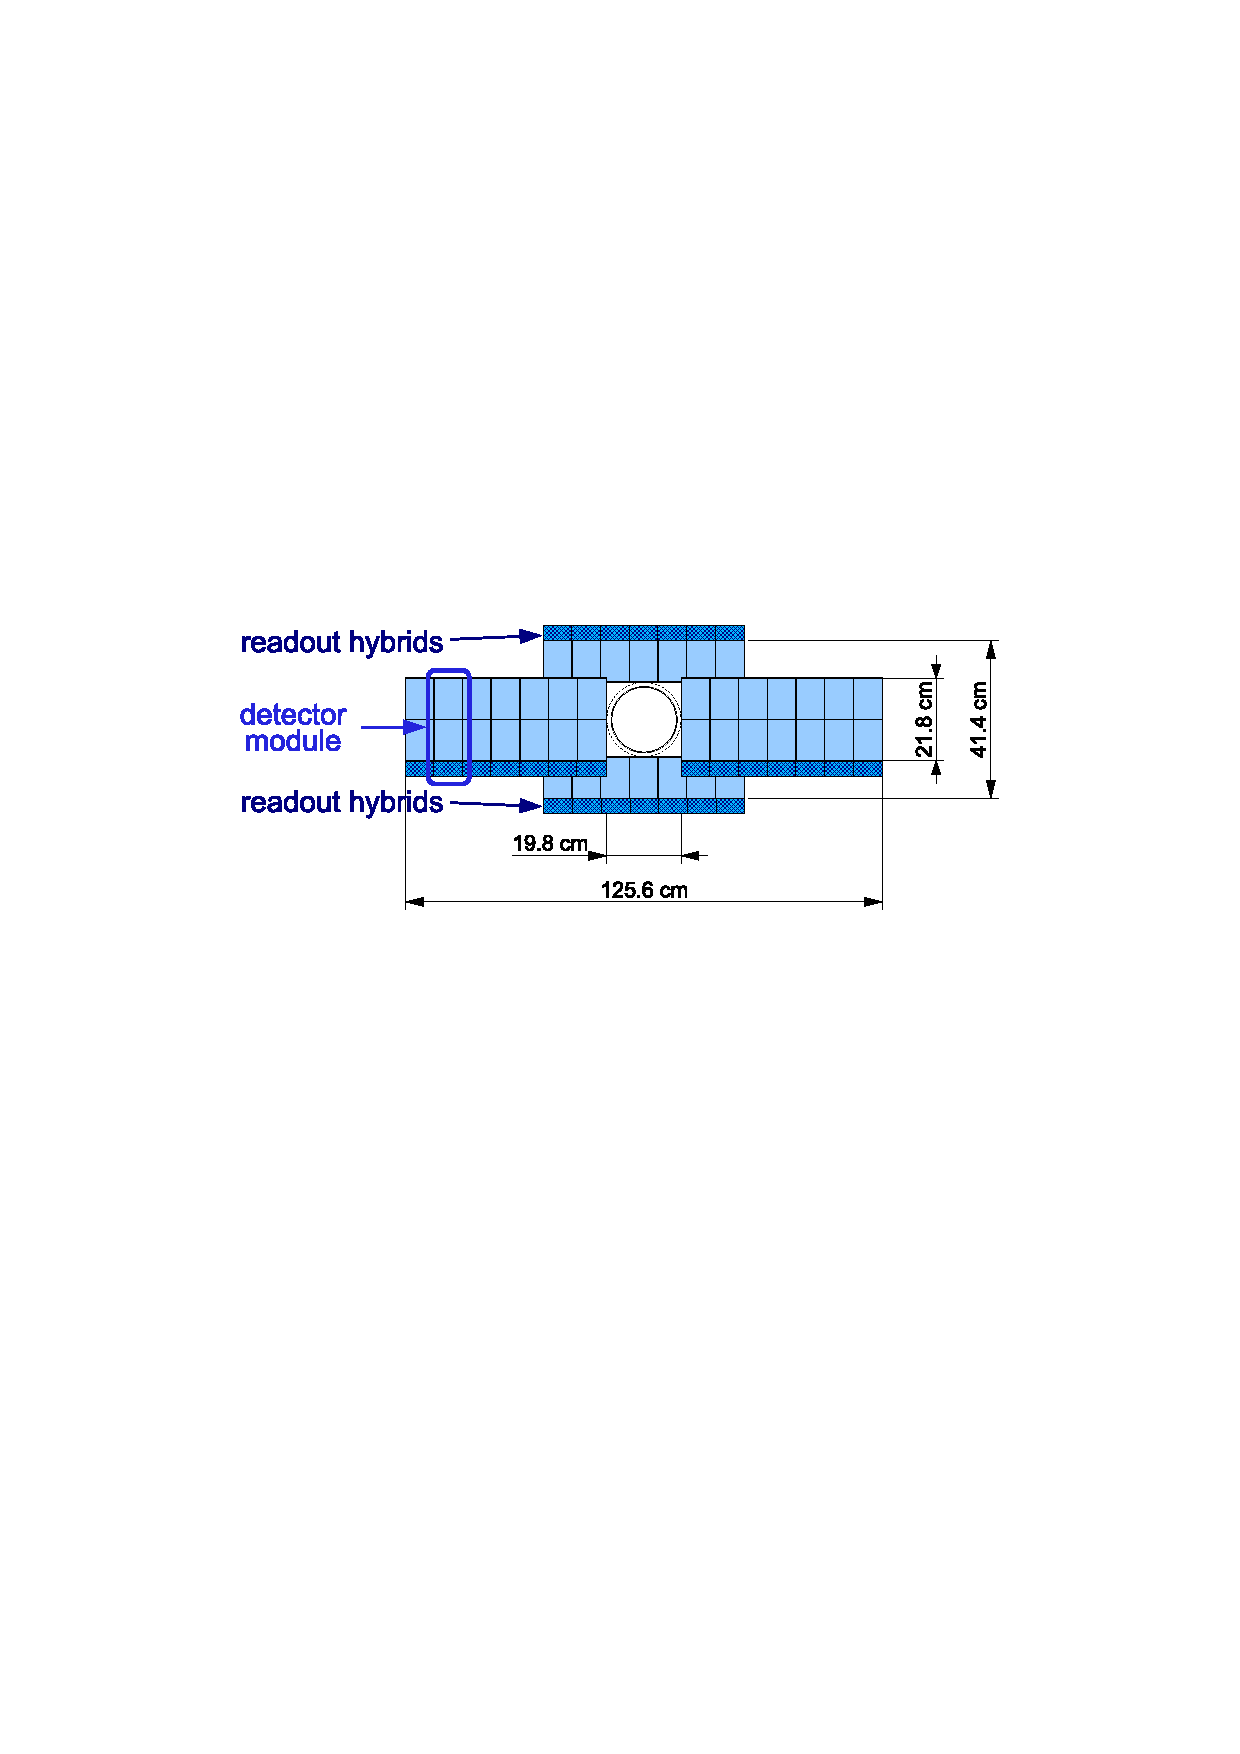
\includegraphics[width=1.0\textwidth]{figs/Detector/it_layout.pdf}
    \end{subfigure}
    \begin{subfigure}[m]{0.49\textwidth}
        \centering
        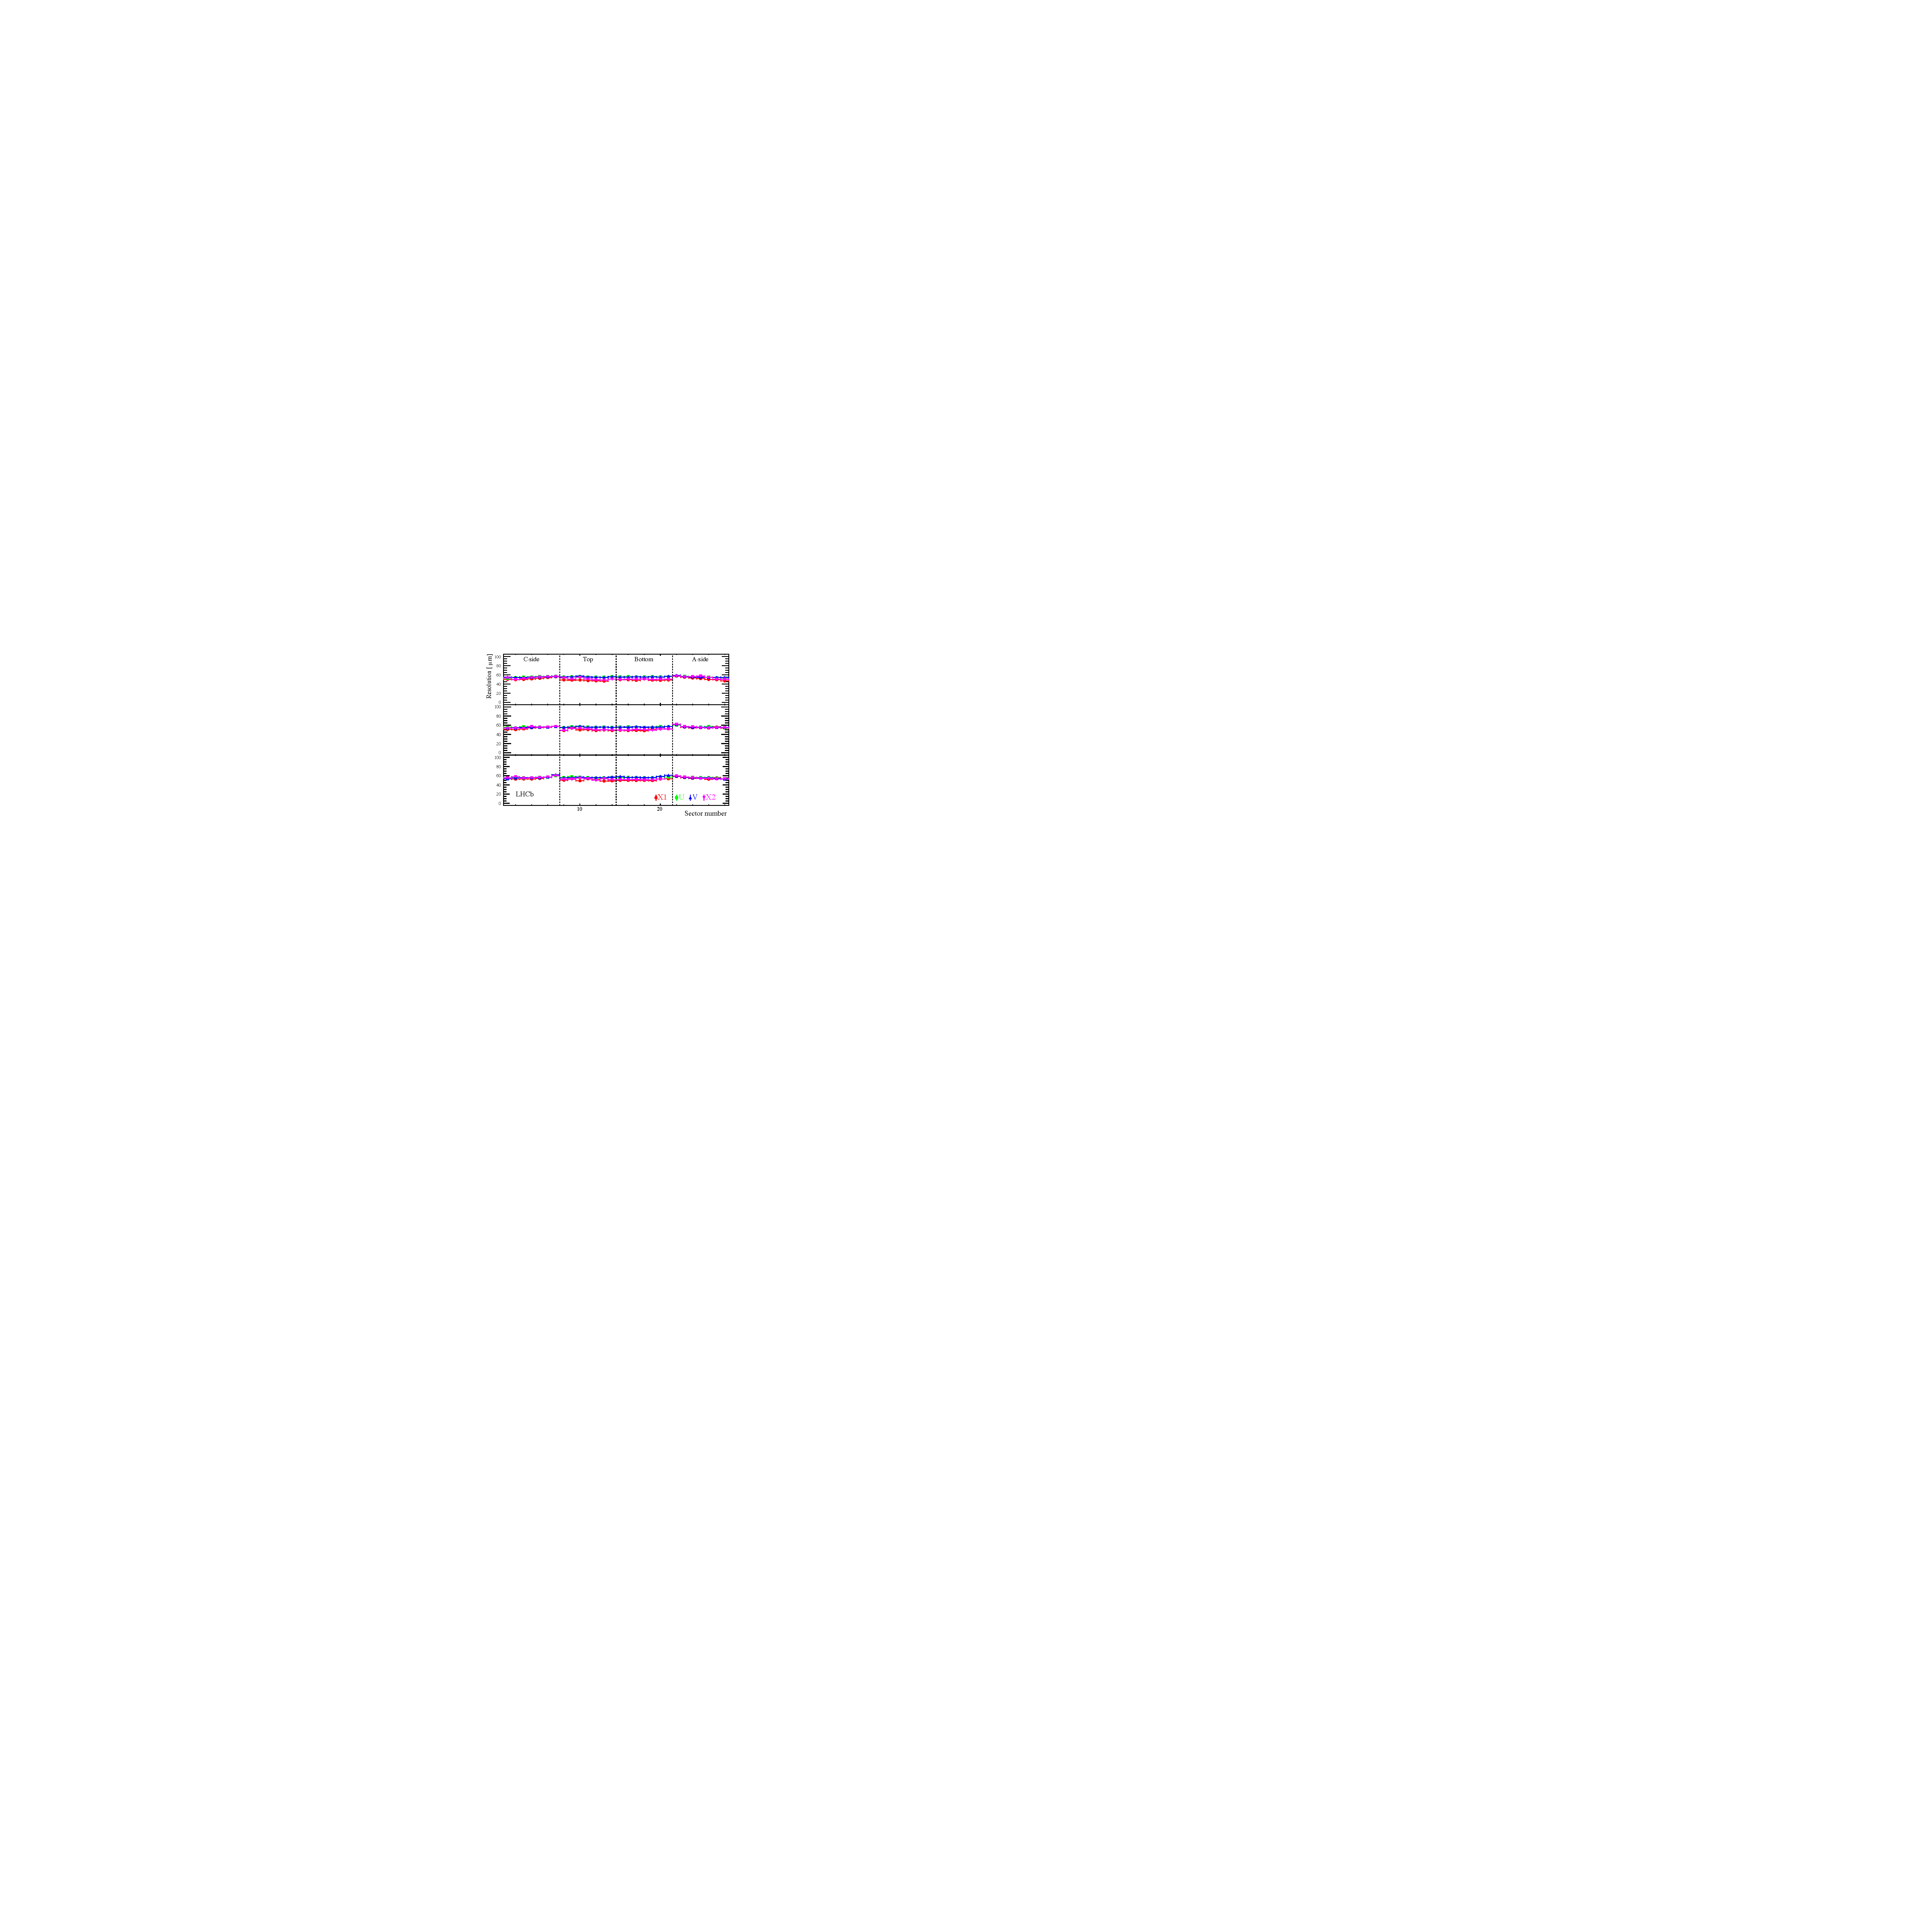
\includegraphics[width=1.0\textwidth]{figs/Detector/it_resolution.pdf}
    \end{subfigure}
    \caption{Schematic of the \intr sub-detector, from Ref.~\cite{Alves:2008zz} (left) and the \intr resolution by sector number, from Ref.~\cite{LHCb-DP-2014-002}.}
    \label{fig:Dec_it_scematic}   
\end{figure}
%%%%%%%%%%%%%%%%%%%%%%%%%%%%%%%%%%%%%%%%%%%%%%%%%%%%%%%%%%



The detector modules consist of either one or two silicon sensors and a readout chip. These are also offset along the beam axis to allow the modules to overlap slightly in the $x$-axis.

The resolution of the \intr is shown in Fig.~\ref{fig:Dec_it_scematic}. The resolution is between 40--60\mum and varies slightly between the four different layers.    



\subsection{Outer Tracker}

In contrast to the the silicon-based trackers, the Outer Tracker (\ot) is a straw tube tracker filled with a gaseous mixture of argon, carbon dioxide and oxygen. The 4.9\mm diameter straws are 2.4\m in length and arranged in double layers as shown in Fig.~\ref{fig:Dec_ot_schematic}. As with the \intr, the \ot is split into three stations. Each of these stations similarly has four layers arranged at angles to one another $(0\degrees,-5\degrees,+5\degrees,0\degrees)$. The arrangement of the stations and layers are also shown in Fig.~\ref{fig:Dec_ot_schematic}. The inner region occupied by the \intr is visible for scale.

%%%%%%%%%%%%%%%%%%%%%%%%%%%%%%%%%%%%%%%%%%%%%%%%%%%%%%%%%%
\begin{figure}[!h]
    \centering
    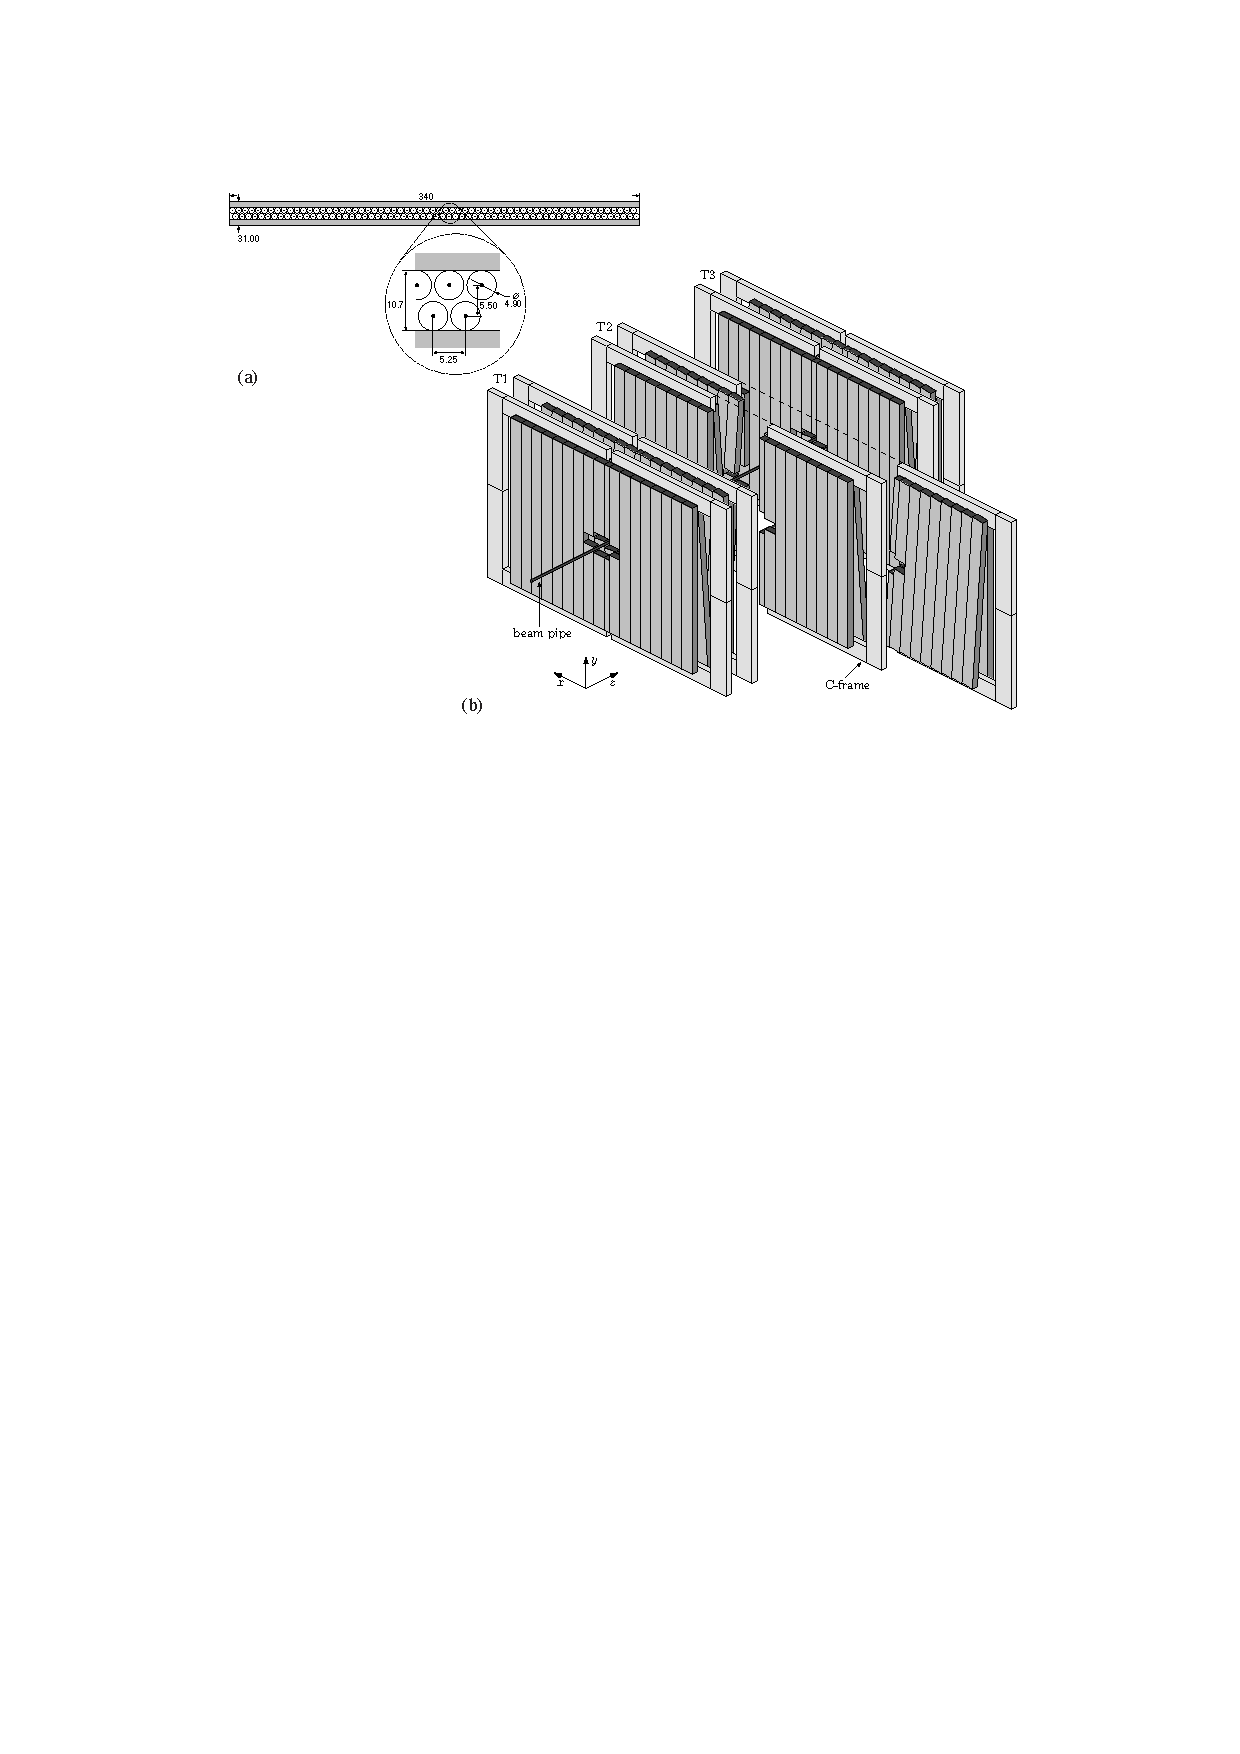
\includegraphics[width=0.8\textwidth]{figs/Detector/ot_layout.pdf}
    \caption{Schematic of the \ot sub-detector, from Ref.~\cite{LHCb-DP-2013-003}.}
    \label{fig:Dec_ot_schematic}   
\end{figure}
%%%%%%%%%%%%%%%%%%%%%%%%%%%%%%%%%%%%%%%%%%%%%%%%%%%%%%%%%%
 
The straws comprising the tracker are composed of an inner wire surrounded by a conducting foil, with a potential difference maintained between the two. When a charged particle passes through the straw the gas becomes ionised. The electrons and gas ions are attracted to the cathode foil and anode wire, resulting in a flow of current. In the \ot the inner wire is made of 25\mum thick gold plated tungsten and maintained at a voltage of +1550\,V. The surrounding foil is made up of three layers; a 40\mum thick layer of conducting carbon-doped polyimide film; a 12.5\mum layer of insulating polyimide; and 12.5\mum of aluminium. 

The double layers of straw tubes as shown in Fig.~\ref{fig:Dec_ot_schematic} make up a module. Vertically, the modules are split in two, with staggered gaps between the two individual straw layers to avoid an uninstrumented region. Each of the modules are read out from the outermost end. 
The readout boards contain a number of circuits to process the signals and provide the potential difference to the straw wires.
The analogue signals pass through an amplification circuit before being processed and cleaned. These then pass into a digitiser creating a digital value of the drift-time.   

The single hit resolution of 205\mum is determined for the \ot by determining the width of the hit distance residual distribution. This is shown in Fig.~\ref{fig:Dec_ot_resolution}.



%%%%%%%%%%%%%%%%%%%%%%%%%%%%%%%%%%%%%%%%%%%%%%%%%%%%%%%%%%
\begin{figure}[!h]
    \centering
    \begin{subfigure}[t]{0.4\textwidth}
        \centering
        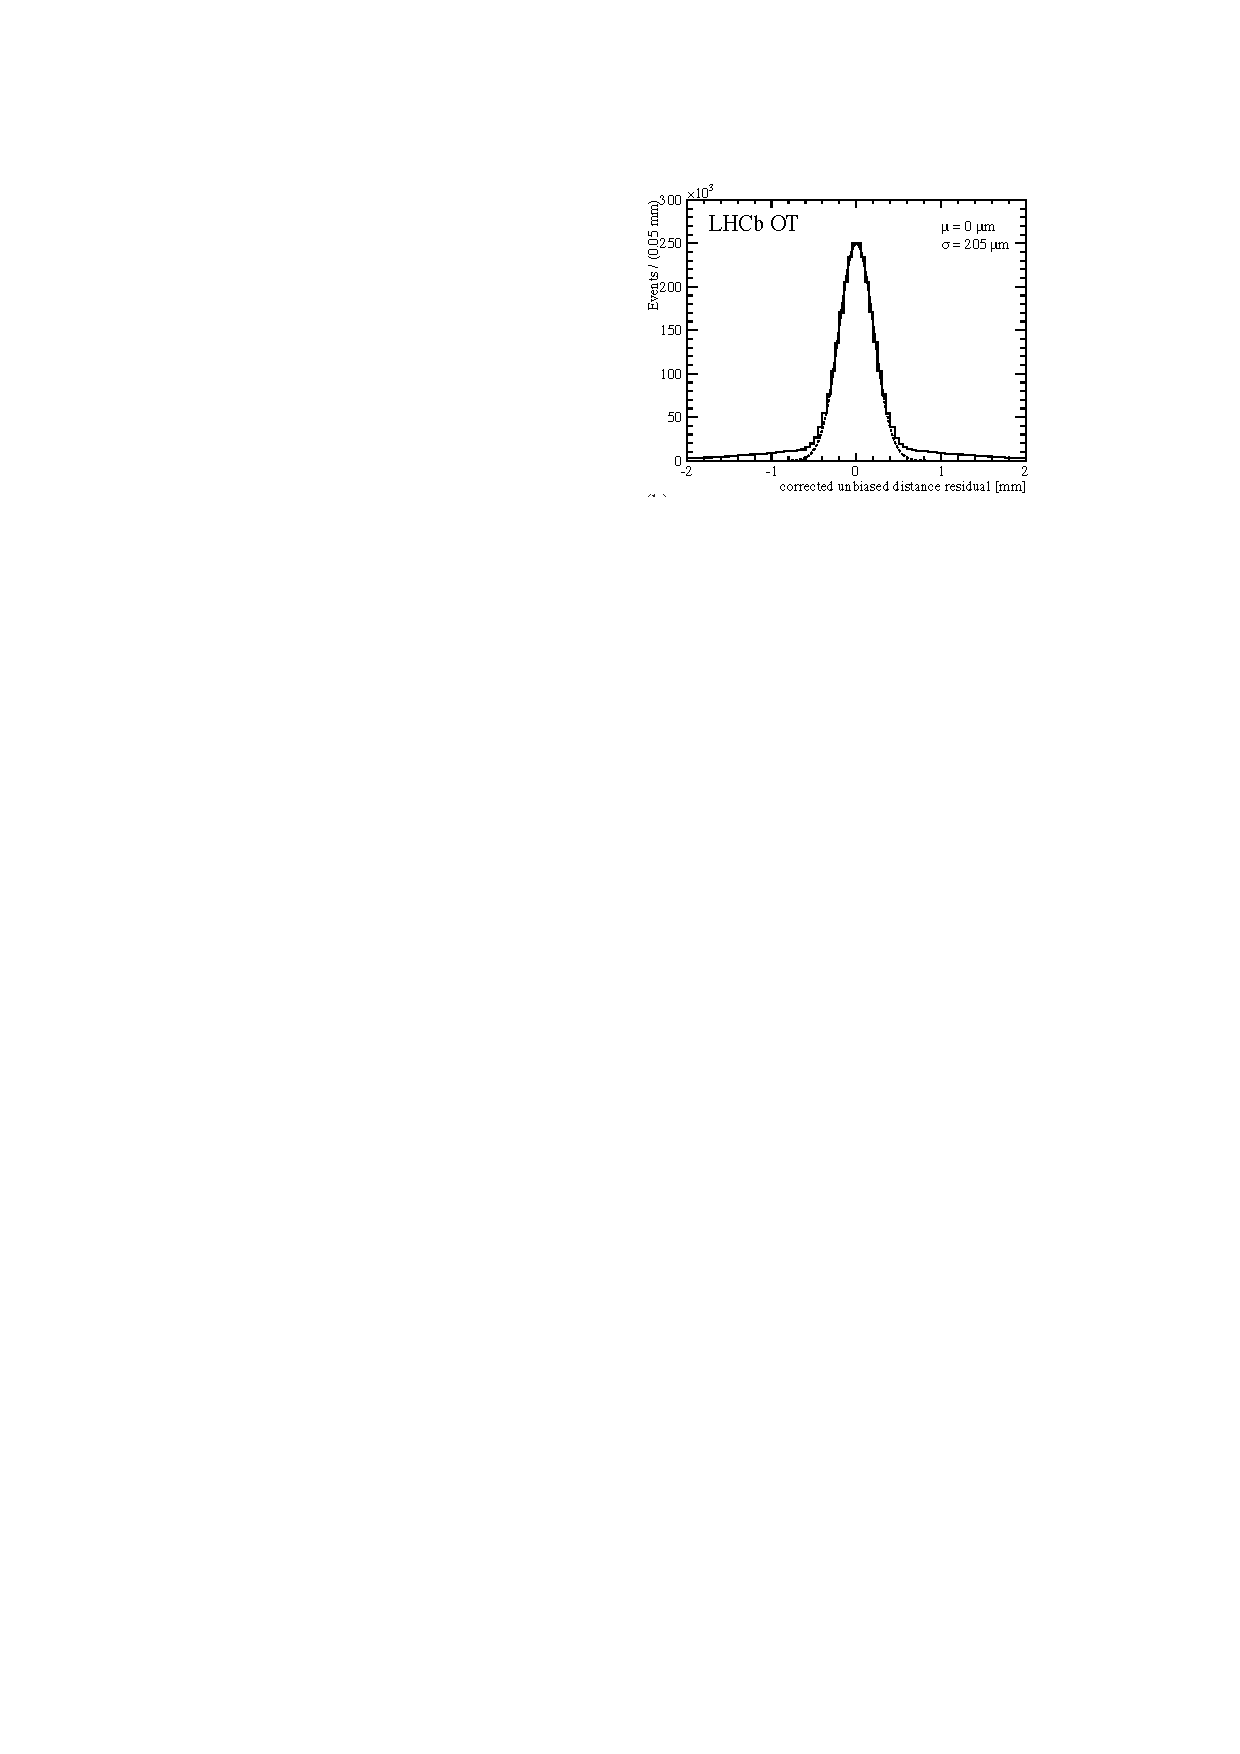
\includegraphics[width=1.0\textwidth]{figs/Detector/ot_residuals.pdf}
    \end{subfigure}
    \caption{The hit distance residuals for the \ot, from Ref.~\cite{LHCb-DP-2013-003}.}
    \label{fig:Dec_ot_resolution}   
\end{figure}
%%%%%%%%%%%%%%%%%%%%%%%%%%%%%%%%%%%%%%%%%%%%%%%%%%%%%%%%%%




% %%%%%%%%%%%%%%%%%%%%%%%%%%%%%%%%%%%%%%%%%%%%%%%%%%%%%%%%%%
% \begin{figure}[!h]
%     \centering
%     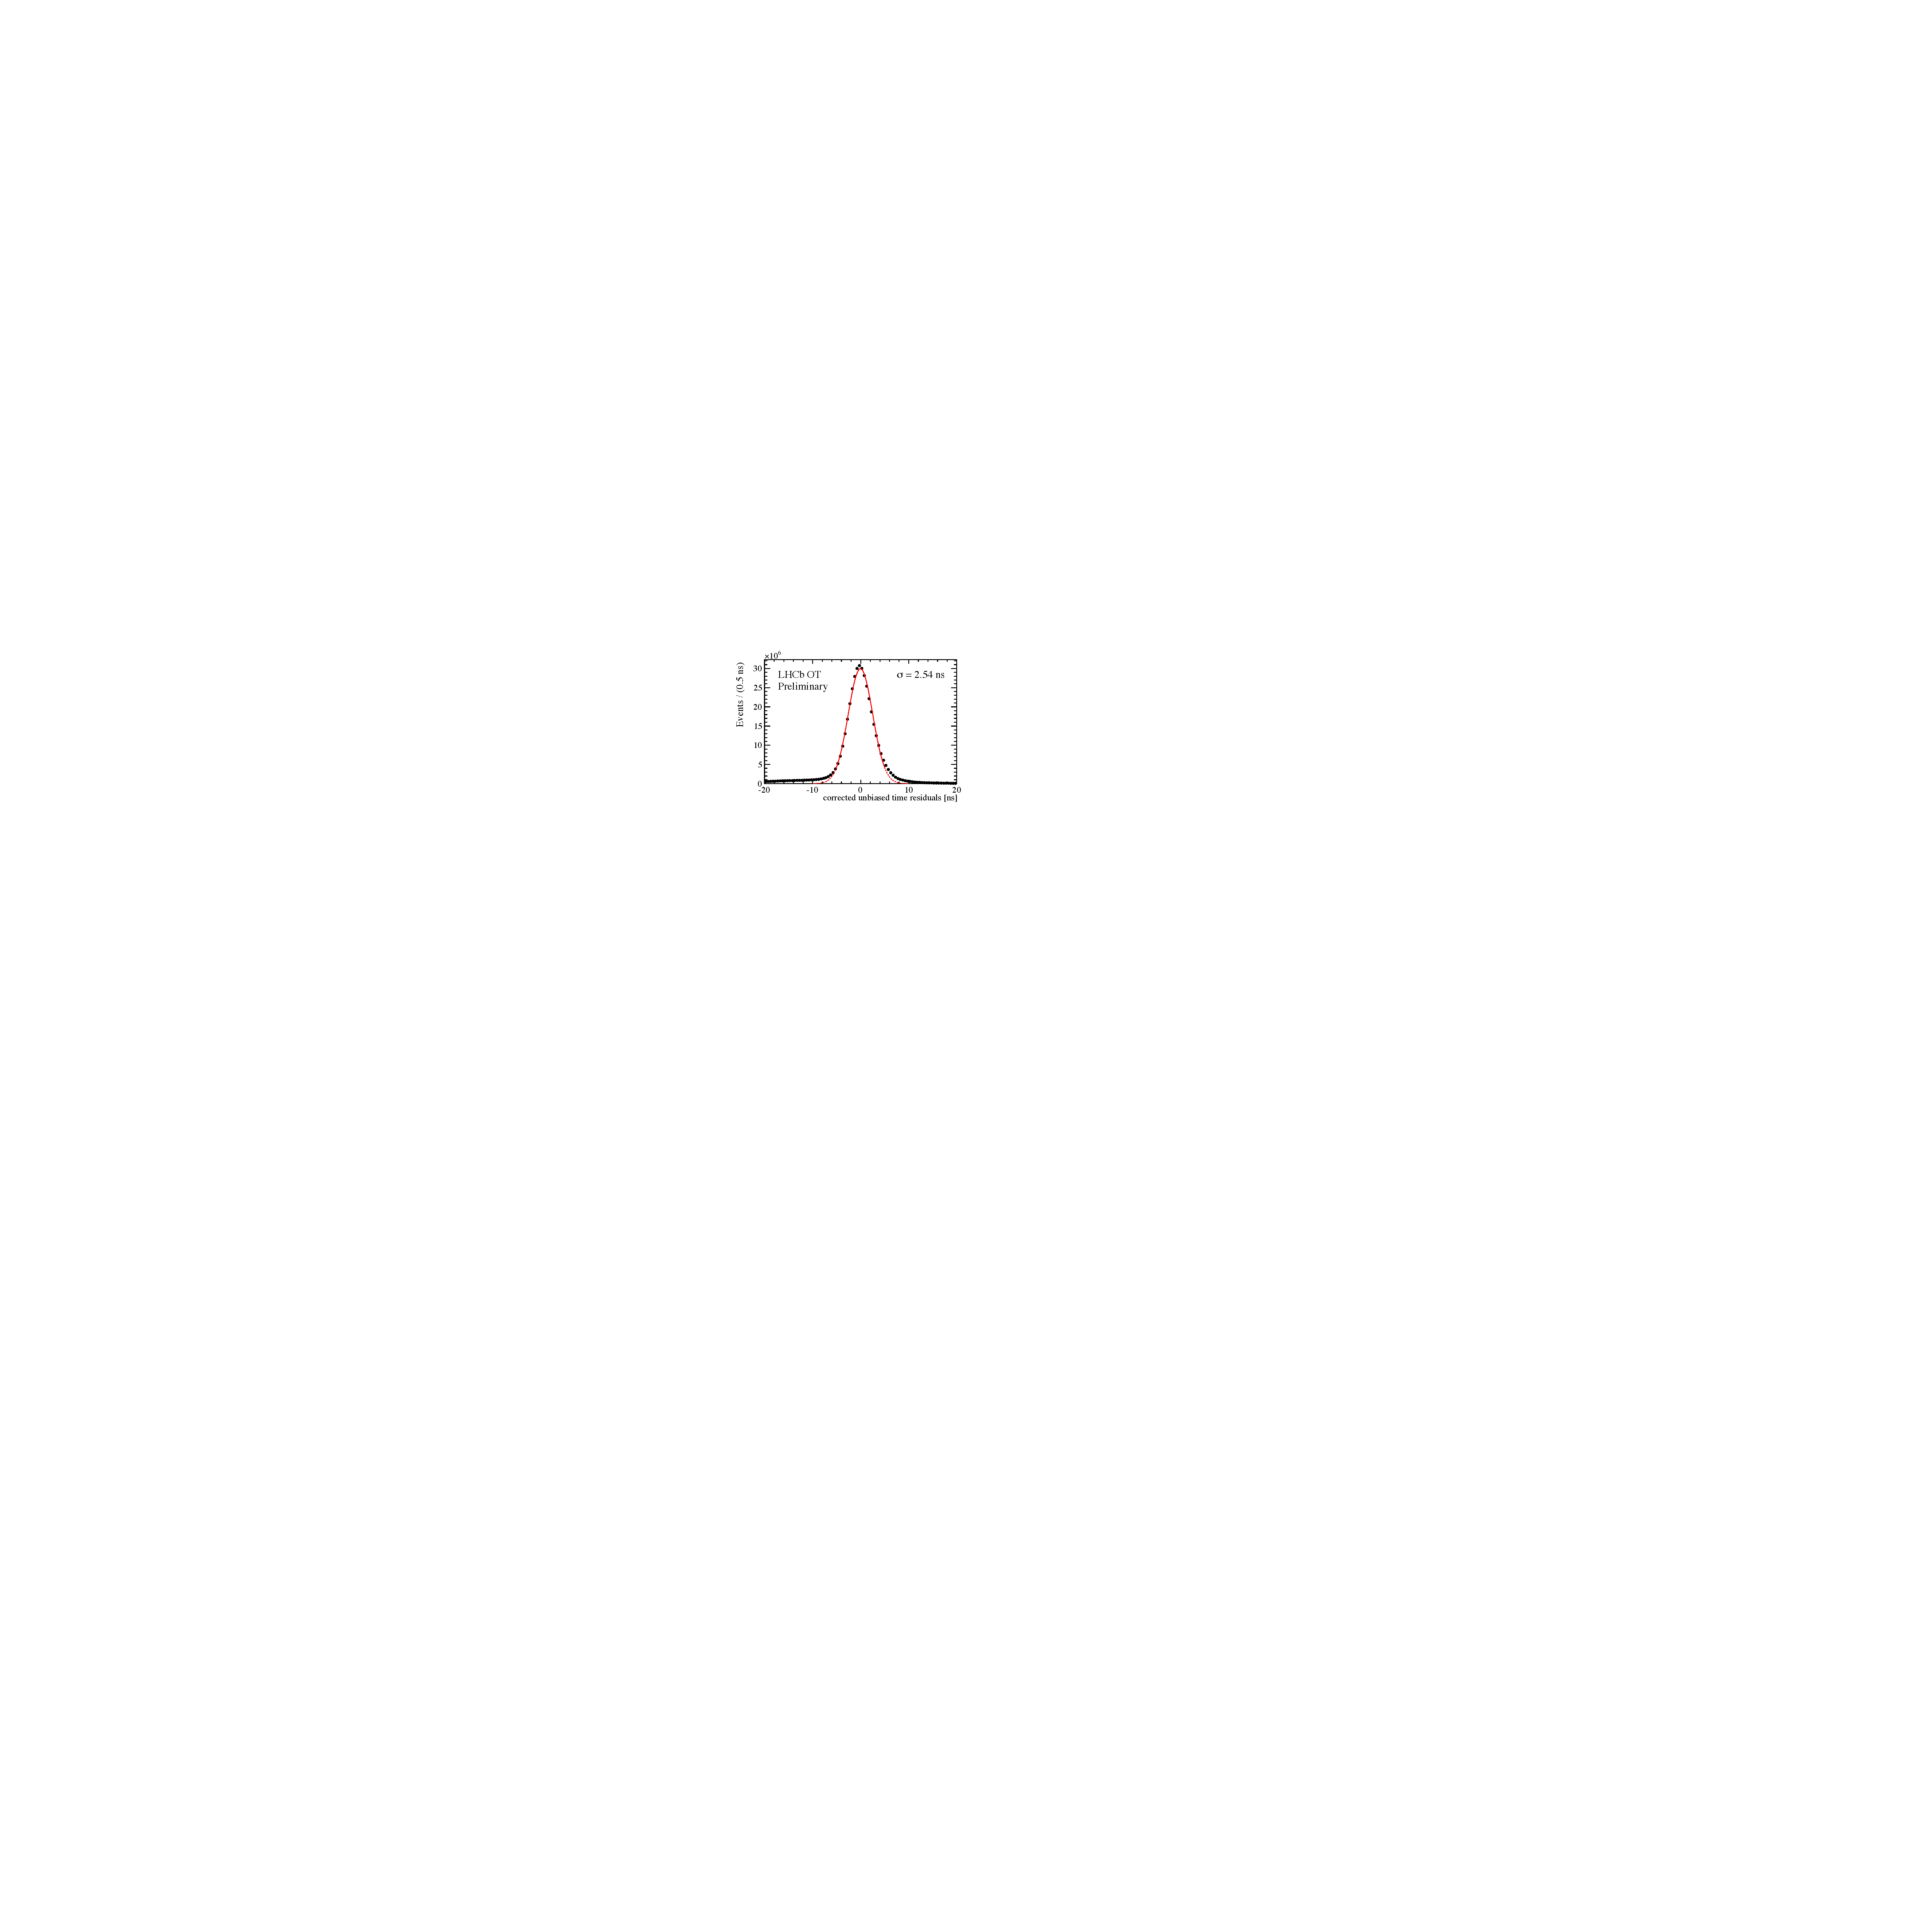
\includegraphics[width=0.6\textwidth]{figs/Detector/ot_resolution.pdf}
%     \caption{The \ttracker resolution, from Ref.~\cite{LHCb-DP-2014-002}.}
%     \label{fig:Dec_velo_leakage_current}   
% \end{figure}
% %%%%%%%%%%%%%%%%%%%%%%%%%%%%%%%%%%%%%%%%%%%%%%%%%%%%%%%%%%


\subsection{Ring imaging Cherenkov detectors}
\label{sec:Dec_RICH}
The ring imaging Cherenkov detectors (\rich) provide dedicated particle identification, which allows different hadronic species to be distinguished.
Kaons, pions and protons are distinguished when the Cherenkov information is coupled with a momentum measurement. It can also help differentiate leptonic tracks in combination with the calorimeters and muon systems. 

Two \rich sub-detectors are needed to cover the track momentum range of \lhcb. The first, \richone, is located between the \velo and \ttracker, before the particles have passed through the magnetic field. This provides discrimination primarily for low momentum tracks between 1--60\gevc. A second sub-detector, \richtwo, is located between the \intr and \ot tracking stations and calorimeters, after the particles have travelled through the magnetic field. This caters for the higher momentum particles in the range 15--100\gevc. 

The \rich detectors determine the species of particles by capturing Cherenkov radiation they emit as they traverses a transparent medium referred to as a radiator. Cherenkov radiation is produced by any particle travelling above the phase velocity of light in that specific medium. The radiation propagates at constant angle $\theta$ to the particles direction, determined by the speed of the particle $\beta = v/c$ and refractive index of the material $n$ as follows
\begin{equation}
\cos{\theta} = \frac{1}{\beta n}.
\end{equation}
This light is collected by mirrors and focussed onto photon detectors. 

Although the particles produced in the collisions are all highly energetic and travelling close to the speed of light, the differences in the masses mean the species travel at slightly difference velocities. This then results in a different Cherenkov angle. In combination with the momentum measurement from the magnet spectrometer, the likelihood of different mass hypotheses can be compared. The Cherekov angles for different particle species as a function of momentum are shown in Fig.~\ref{fig:Dec_rich_species}. 


%%%%%%%%%%%%%%%%%%%%%%%%%%%%%%%%%%%%%%%%%%%%%%%%%%%%%%%%%%
\begin{figure}[!h]
    \centering
    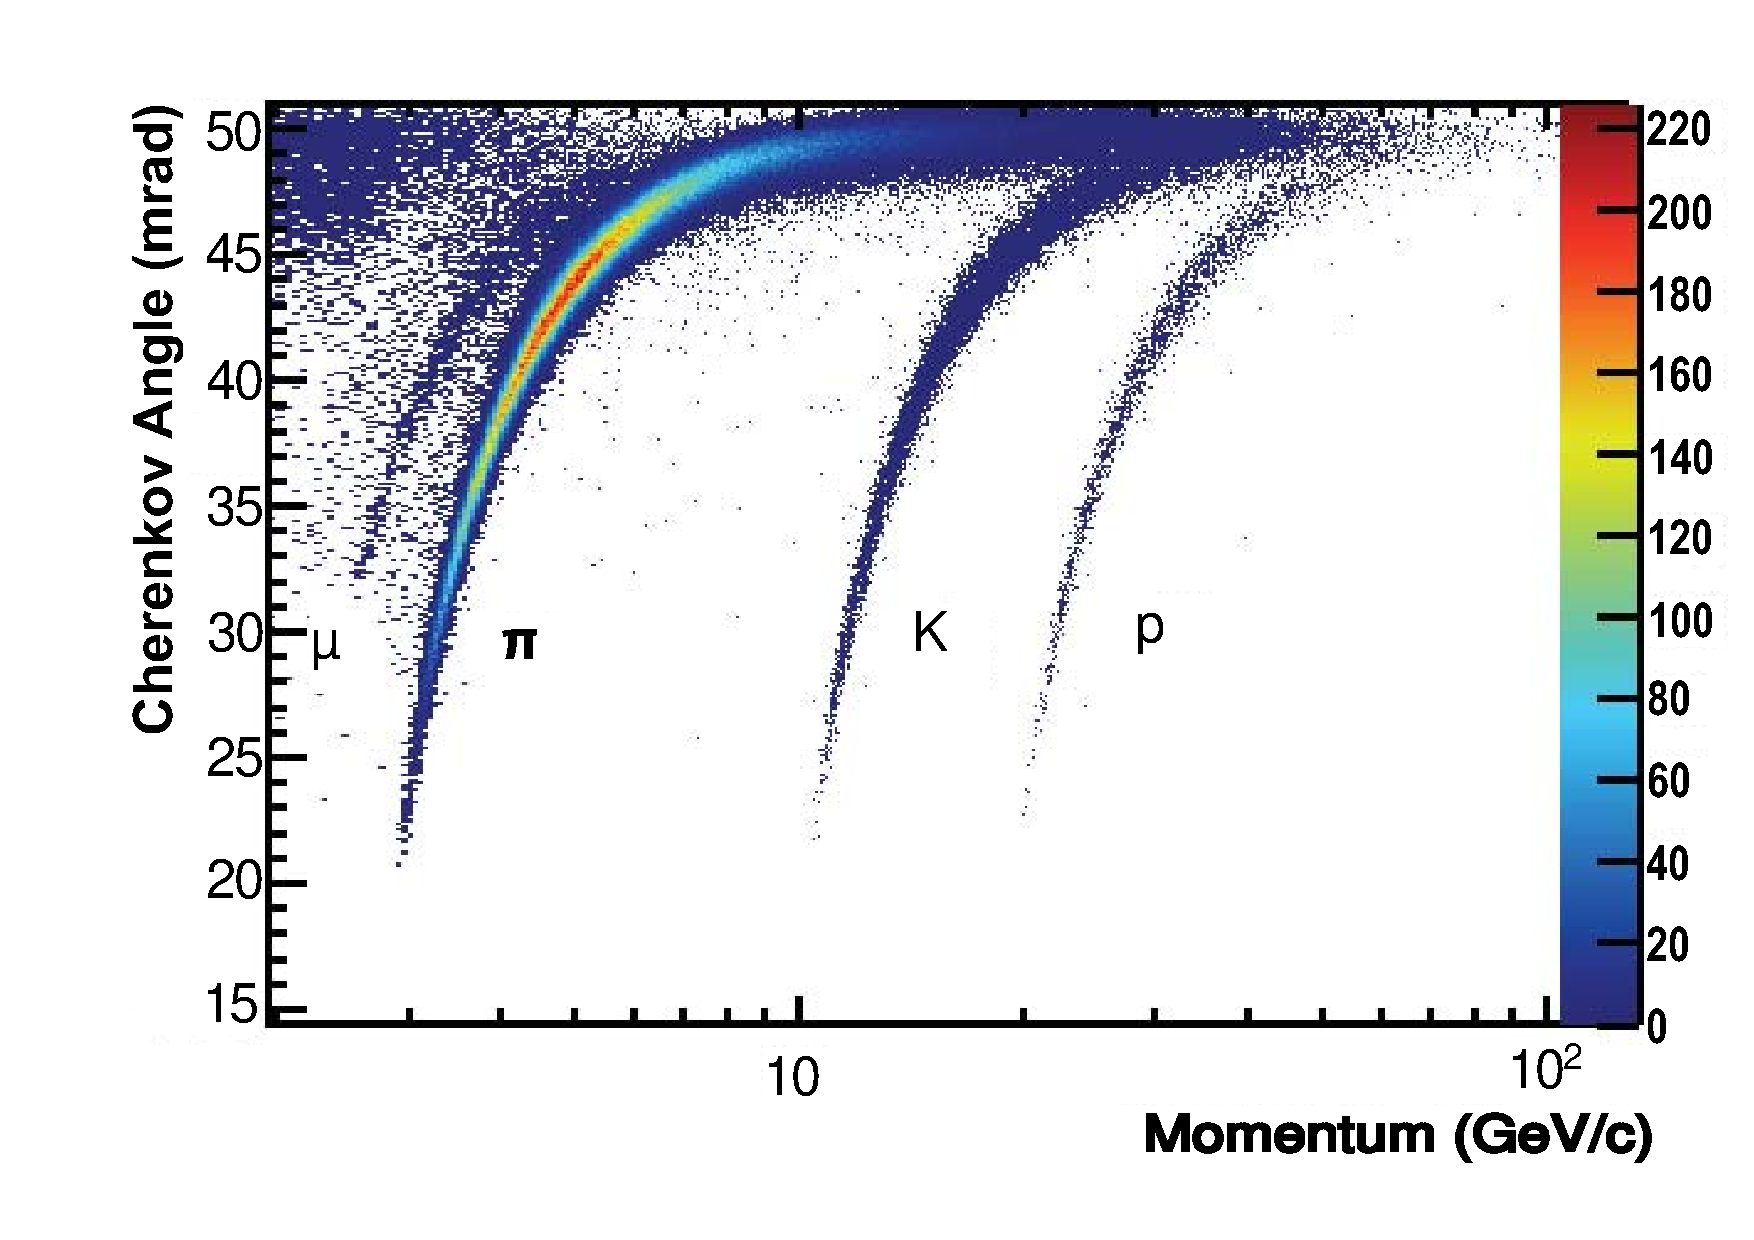
\includegraphics[width=0.6\textwidth]{figs/Detector/rich_speices.pdf}
    \caption{The Cherenkov angle for different species of particles as a function of momentum, from Ref.~\cite{LHCb-DP-2012-003}.}
    \label{fig:Dec_rich_species}   
\end{figure}
%%%%%%%%%%%%%%%%%%%%%%%%%%%%%%%%%%%%%%%%%%%%%%%%%%%%%%%%%%


In both \richone and \richtwo the cone of Cherenkov radiation is reflected off spherical and planar mirrors. This not only redirects the radiation onto Hybrid Photon Detectors (HPDs) situated outside of the acceptance but also focusses the radiation into a single ring.    
The radius of this ring is used to determine the Cherenkov angle $\theta$. 
The identity of particles is determined by comparing likelihood for a given ring of hits to have been created by various species. 
This is performed globally for all tracks in an event. All tracks are assumed to be pions as these are most abundant. The hypothesis of each is switched to $e$, $\mu$, $K$ and proton, leaving all other tracks unchanged, and the likelihood recomputed. The species resulting in the maximum value of the global event likelihood is kept. This is repeated until all tracks are set to their preferred hypothesis. 
The difference in the global event log-likelihood is then used to indicate the species of each track. Each species is determined relative to the pion hypothesis 
\begin{equation}
\text{DLL} = \Delta \log{\mathcal{L}(X-\pi)} = \log{\mathcal{L}(X)} - \log{\mathcal{L}(\pi)},
\end{equation}
where $\mathcal{L}(X)$ is the global event likelihood when the given track is of the species $X$.








\subsubsection{\richone}
The \richone sub-detector was designed for tracks in the range 1--60\gevc using two radiators: aerogel and decafluorobutane ($\text{C}_{4}\text{F}_{10}$). These materials have refractive indices of $n = 1.030$ and $n = 1.0014$ respectively for $\lambda = 400\nm$ light. A diagram of the \richone detector as seen from the side is shown in Fig.~\ref{fig:Dec_rich_layout}. To minimise the amount of material that the particles pass through, the \richone detector is attached directly onto the \velo exit window.  

% %%%%%%%%%%%%%%%%%%%%%%%%%%%%%%%%%%%%%%%%%%%%%%%%%%%%%%%%%%
% \begin{figure}[!h]
%     \centering        
%     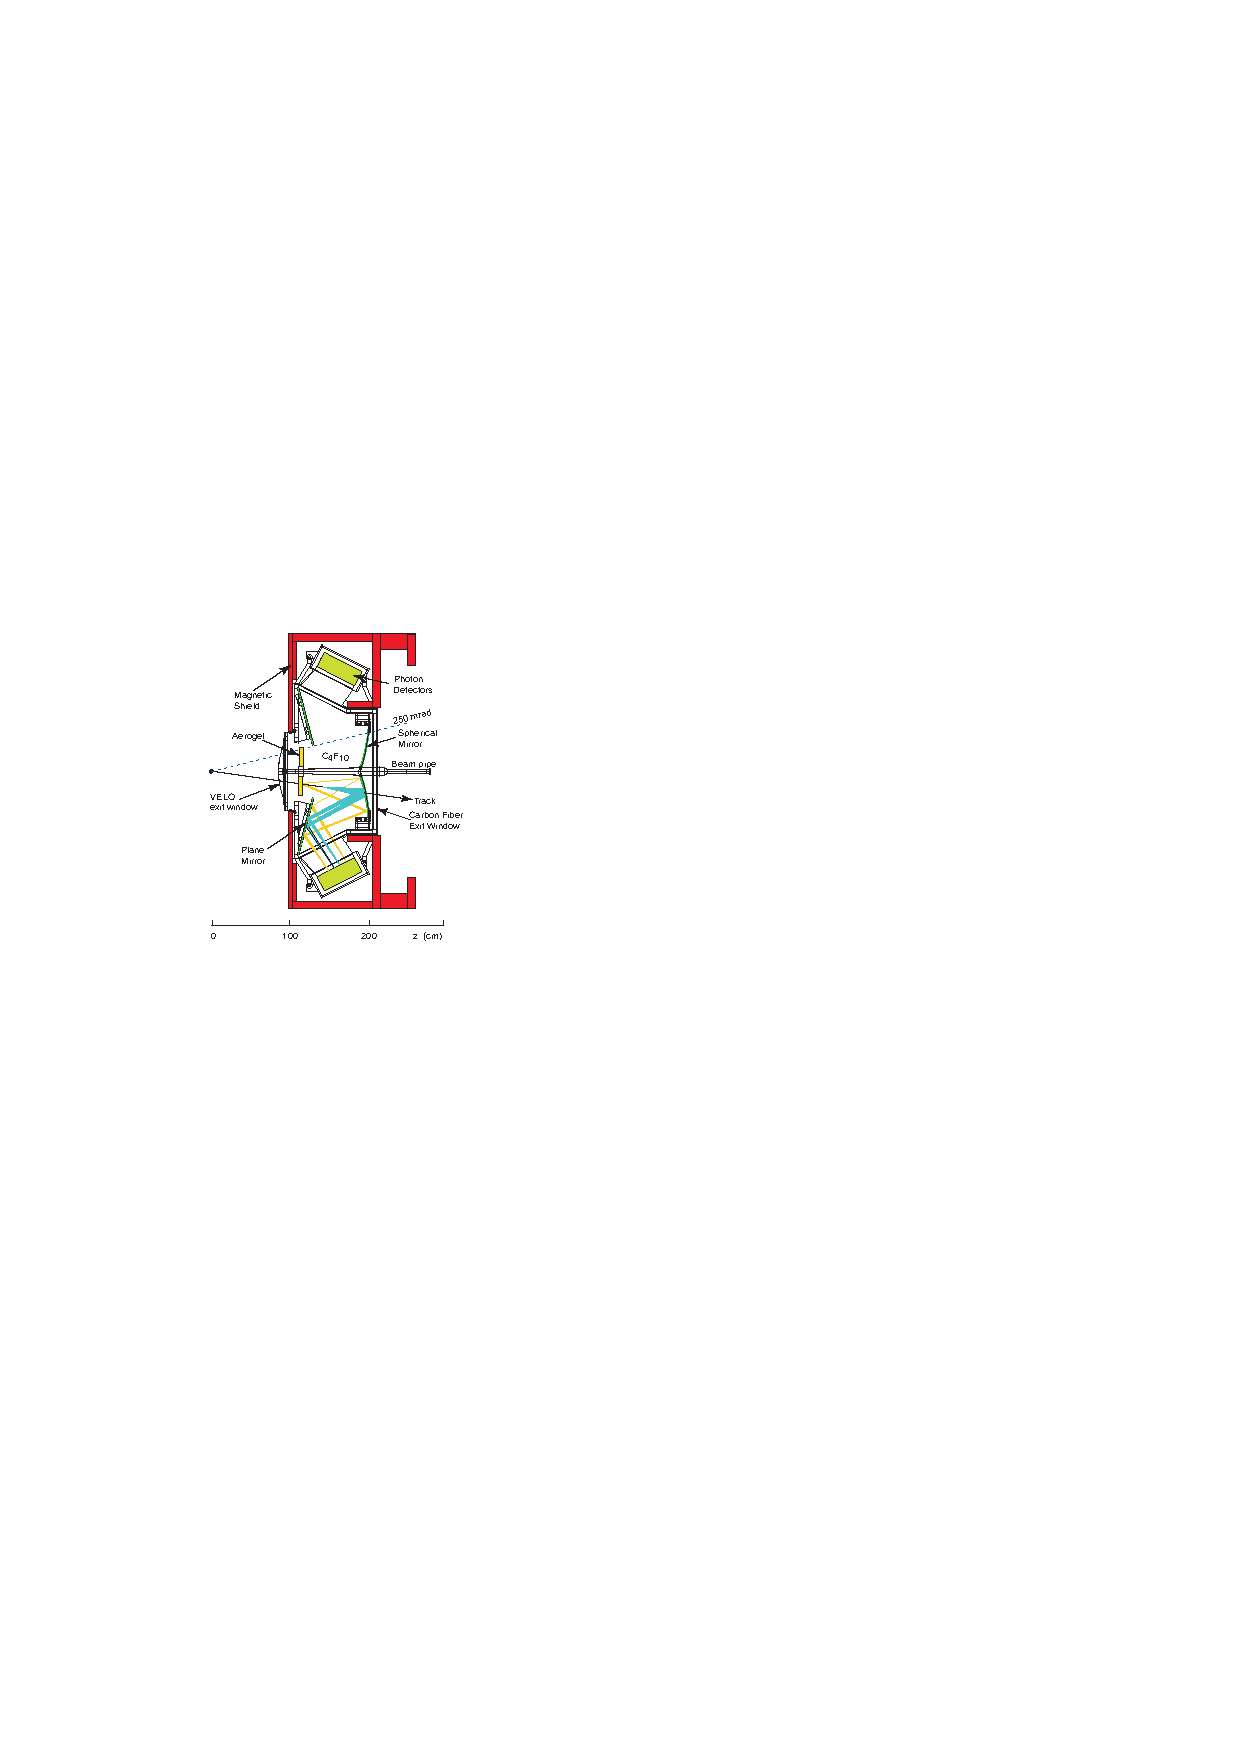
\includegraphics[width=0.4\textwidth]{figs/Detector/richone_layout.pdf}
%     \caption{Schematic the \richone sub-detectors viewed from the side, from Ref.~\cite{Alves:2008zz}.}
%     \label{fig:Dec_richone_layout}   
% \end{figure}
% %%%%%%%%%%%%%%%%%%%%%%%%%%%%%%%%%%%%%%%%%%%%%%%%%%%%%%%%%%
%%%%%%%%%%%%%%%%%%%%%%%%%%%%%%%%%%%%%%%%%%%%%%%%%%%%%%%%%%
\begin{figure}[!h]
    \centering
    \begin{subfigure}[t]{0.4\textwidth}
        \centering        
        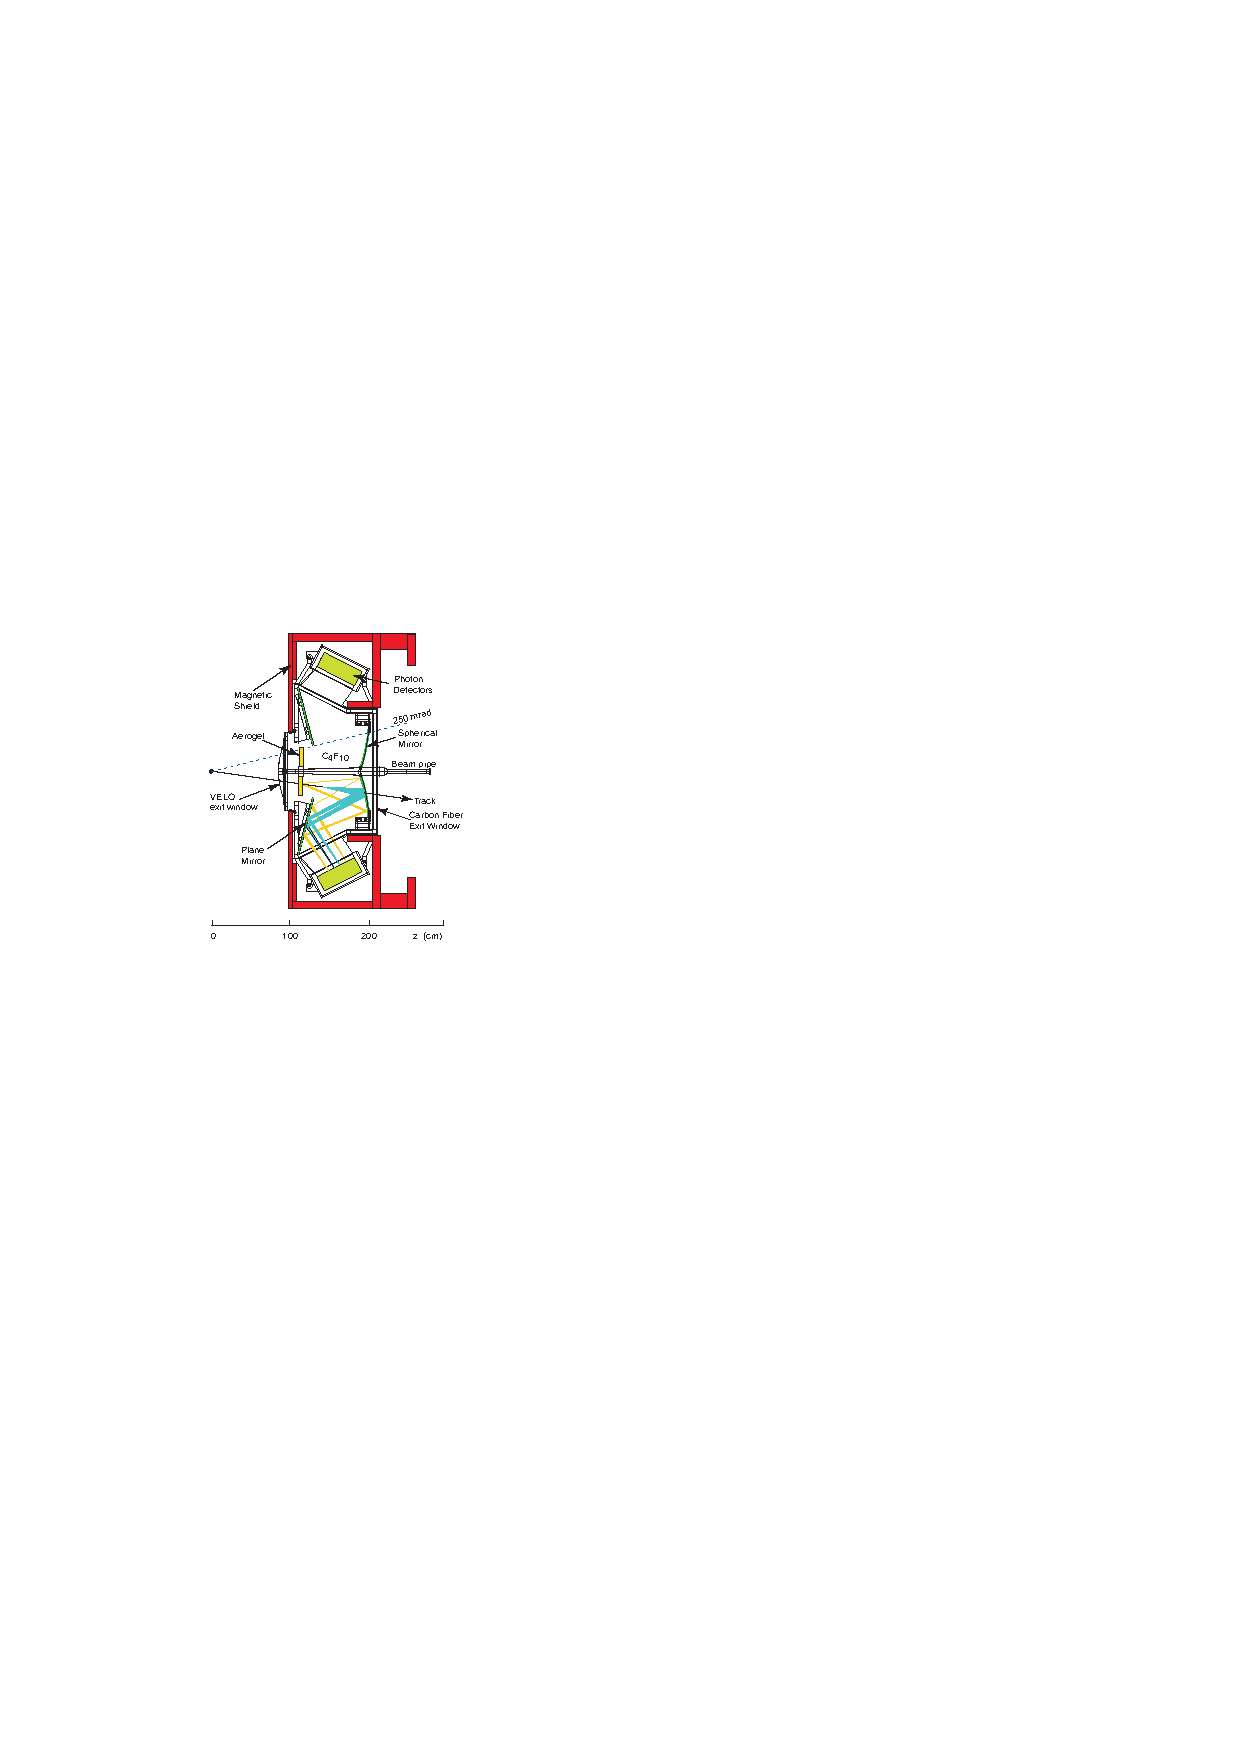
\includegraphics[width=1.0\textwidth]{figs/Detector/richone_layout.pdf}
        \caption{\richone}
    \end{subfigure}
    \begin{subfigure}[t]{0.4\textwidth}
        \centering
        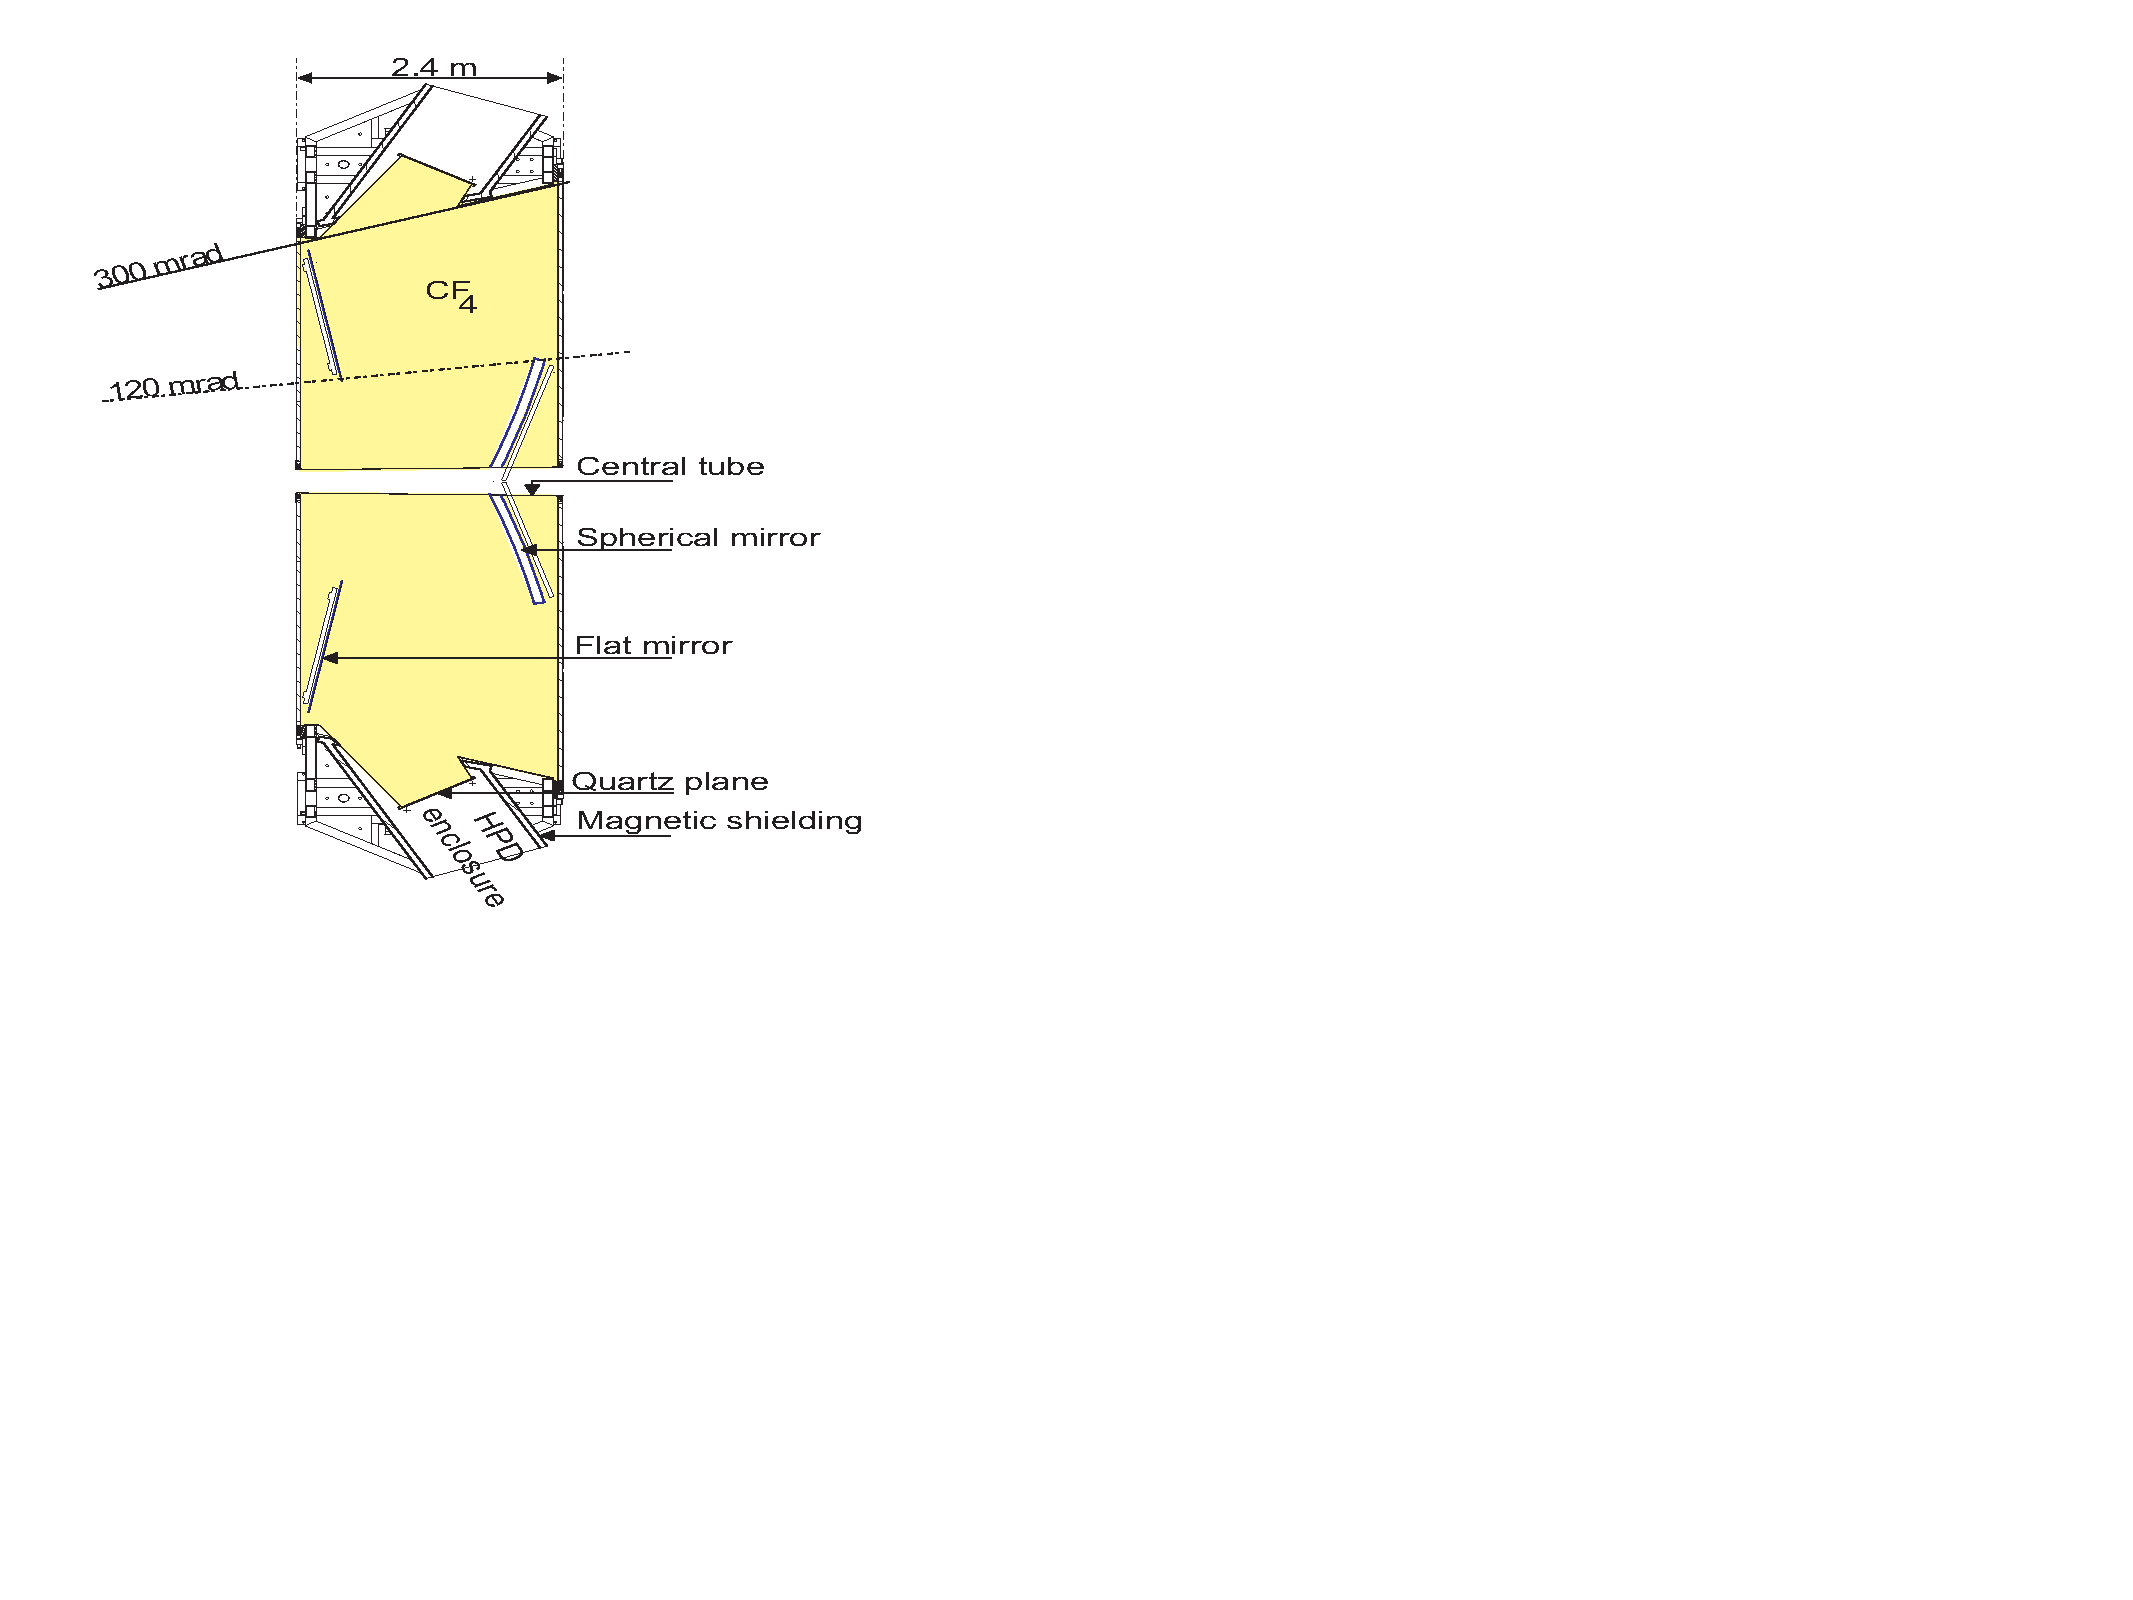
\includegraphics[width=1.0\textwidth]{figs/Detector/richtwo_layout_2.pdf}
        \caption{\richtwo}
    \end{subfigure}
    \caption{Schematic the \richone (left) and \richtwo (right) sub-detectors viewed from the side, from Ref.~\cite{Alves:2008zz}.}

    \label{fig:Dec_rich_layout}   
\end{figure}
%%%%%%%%%%%%%%%%%%%%%%%%%%%%%%%%%%%%%%%%%%%%%%%%%%%%%%%%%%
In Run II the aerogel was removed from the \richone detector. Although this catered specifically to the lower momentum tracks, the overall PID efficiency benefited from less material~\cite{PAPANESTIS2017221}. Compared to design expectations, the ability of the aerogel to provide particle identification for kaons below the $\text{C}_{4}\text{F}_{10}$ threshold was deteriorated by the number of photons in \richone. This was the result of \lhcb running at a higher than anticipated pile up. As well as improving the reconstruction speed, the removal of the aerogel also allows the photons emitted in the aerogel volume to be collected. 

The single photon resolution for \richone is 1.65\mrad, and found to be the same in Run I and Run II. The dominant source of resolution degradation are the finite pixel size, the unknown emission point and the chromatic aberration.  


\subsubsection{\richtwo}

The \richtwo detector is designed to provide particle identification of tracks in the range 15--100\gevc using a gas radiator, tetrafluoromethane ($\text{C}\text{F}_{4}$). The refractive index for this material is $n=1.0005$ for $\lambda = 400\nm$ light.

% %%%%%%%%%%%%%%%%%%%%%%%%%%%%%%%%%%%%%%%%%%%%%%%%%%%%%%%%%%
% \begin{figure}[!h]
%     \centering        
%     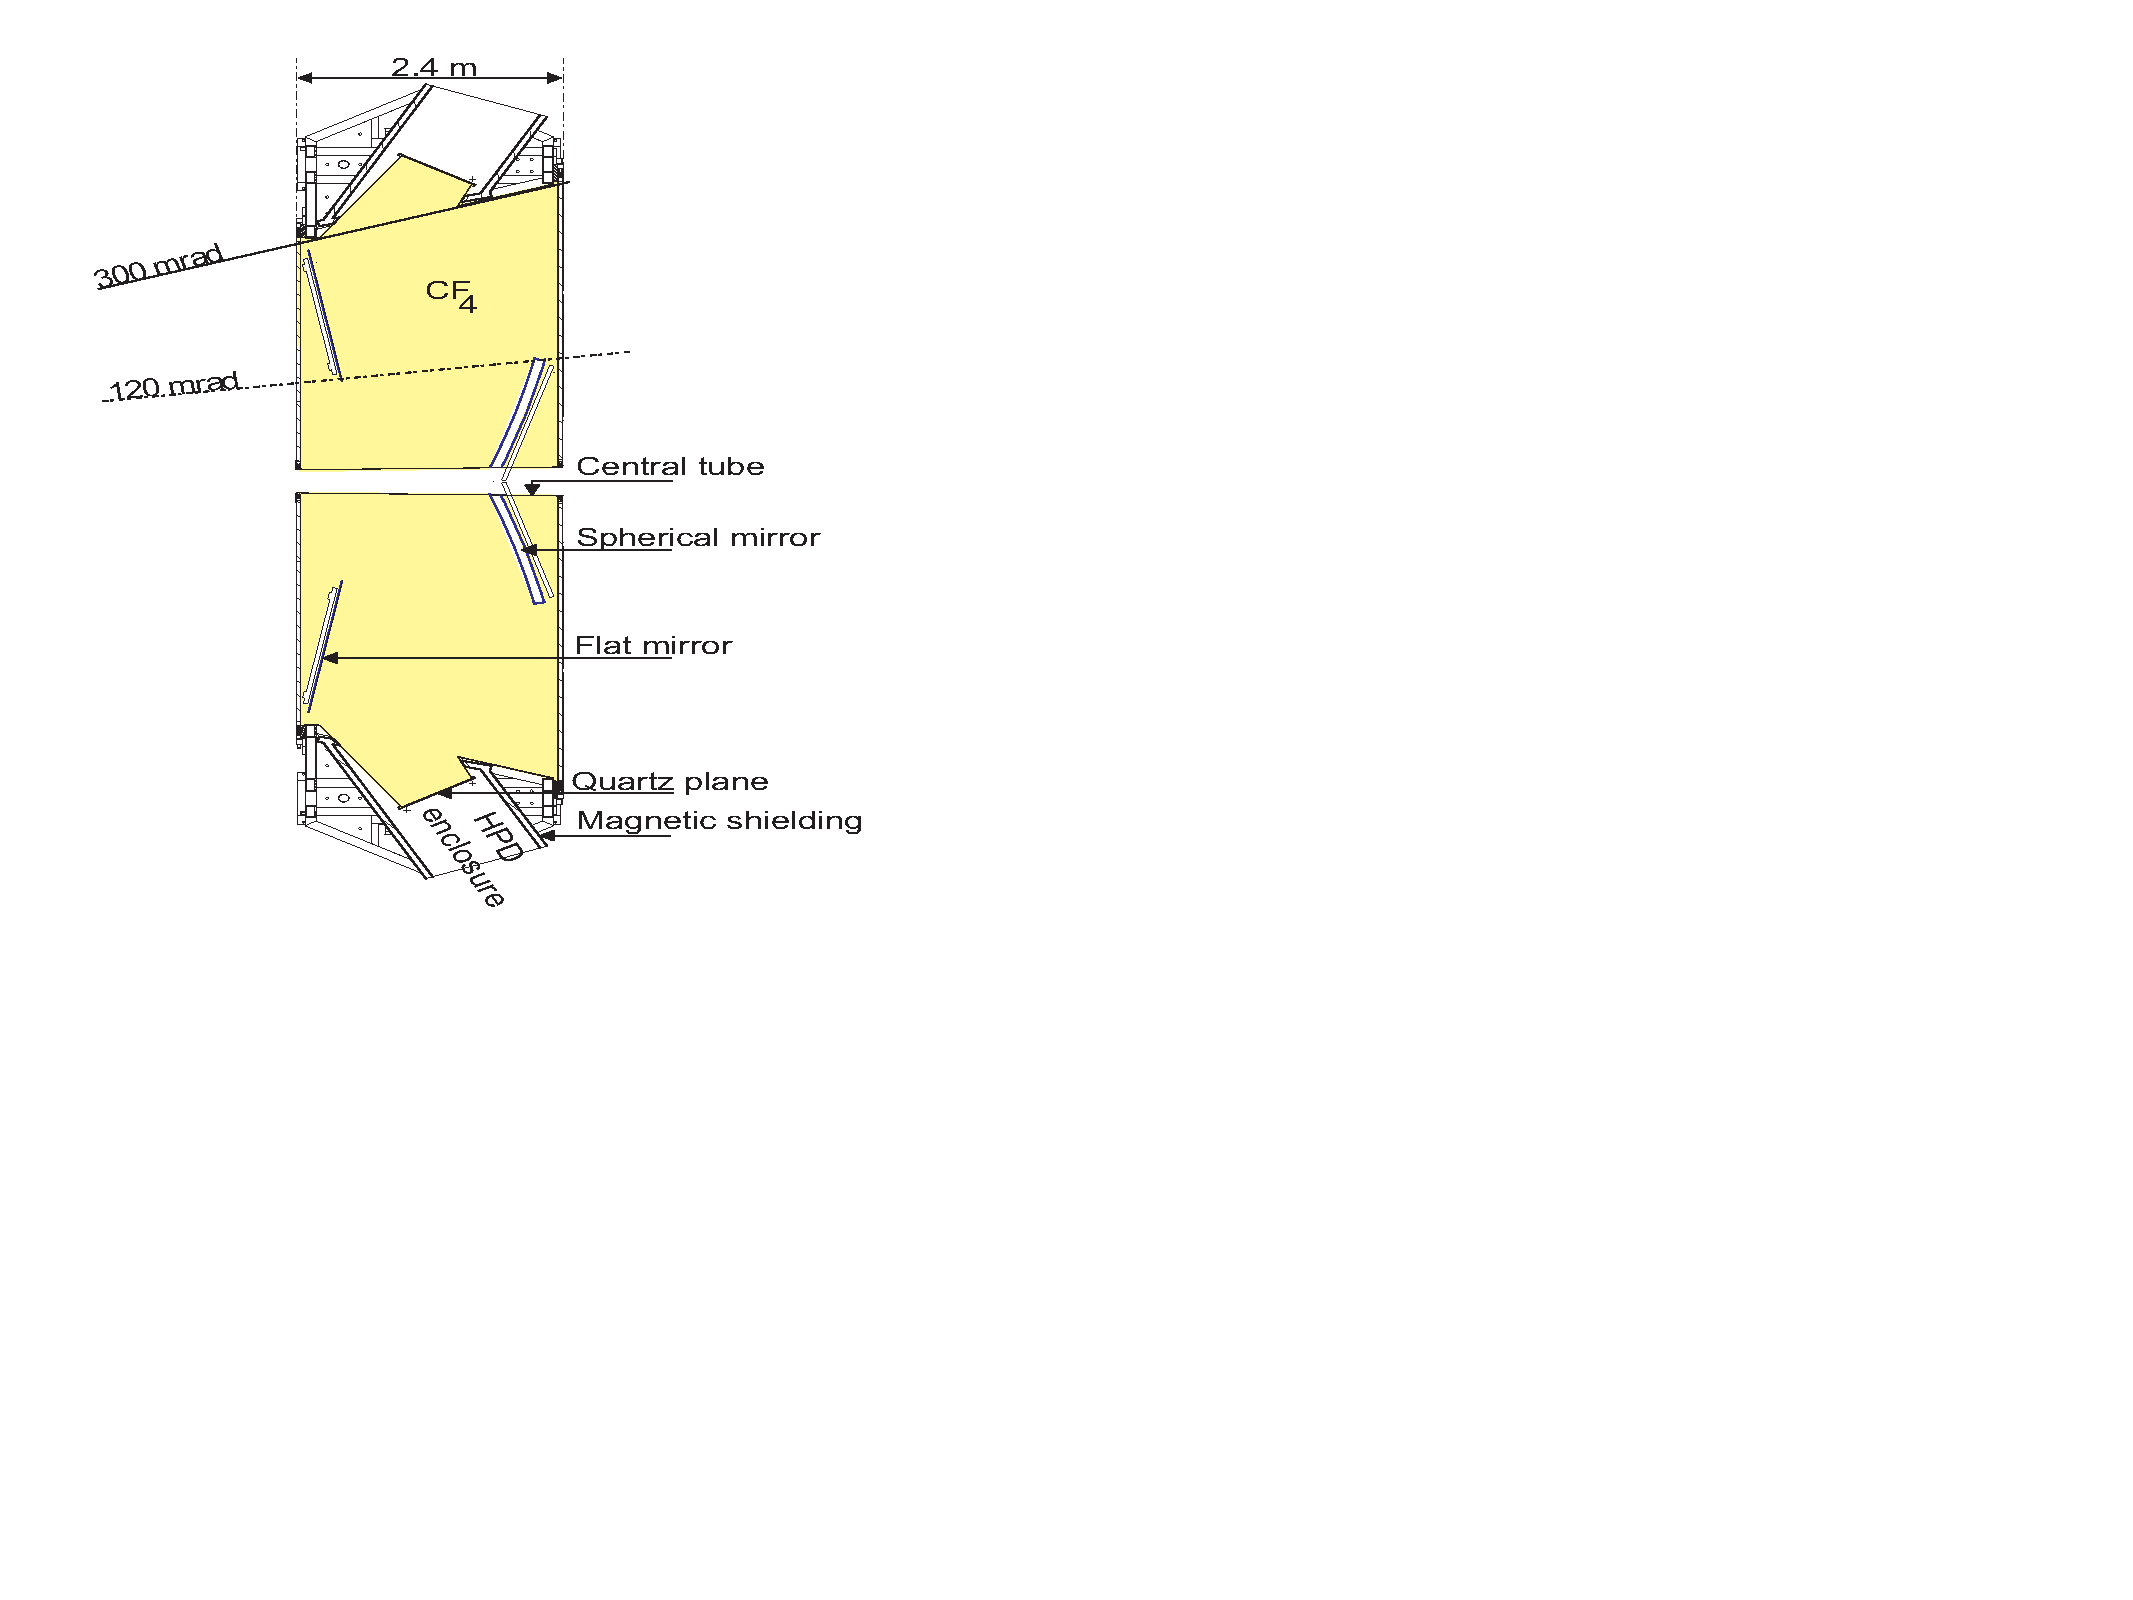
\includegraphics[width=0.4\textwidth]{figs/Detector/richtwo_layout_2.pdf}
%     \caption{Schematic the \richtwo sub-detector viewed from above, from Ref.~\cite{Alves:2008zz}.}
%     \label{fig:Dec_richtwo_layout}   
% \end{figure}
% %%%%%%%%%%%%%%%%%%%%%%%%%%%%%%%%%%%%%%%%%%%%%%%%%%%%%%%%%%
The single photon resolution for \richtwo is 0.67\mrad and found to be consistent between Run I and Run II~\cite{PAPANESTIS2017221}.


\subsubsection{Performance}
The performance of the \rich detectors is quantified in terms of the selection efficiency and misidentification rates for different pairs of species. The efficiency of kaon identification and rate of pions being misidentified as kaons is shown in Fig.~\ref{fig:Dec_rich_k_pi} for Run I and Run II. Due to the removal of the aerogel in \richone, the kaon and pion separation shows an improvement in Run II.

%%%%%%%%%%%%%%%%%%%%%%%%%%%%%%%%%%%%%%%%%%%%%%%%%%%%%%%%%%
\begin{figure}[!h]
    \centering
    \begin{subfigure}[t]{0.4\textwidth}
        \centering        
        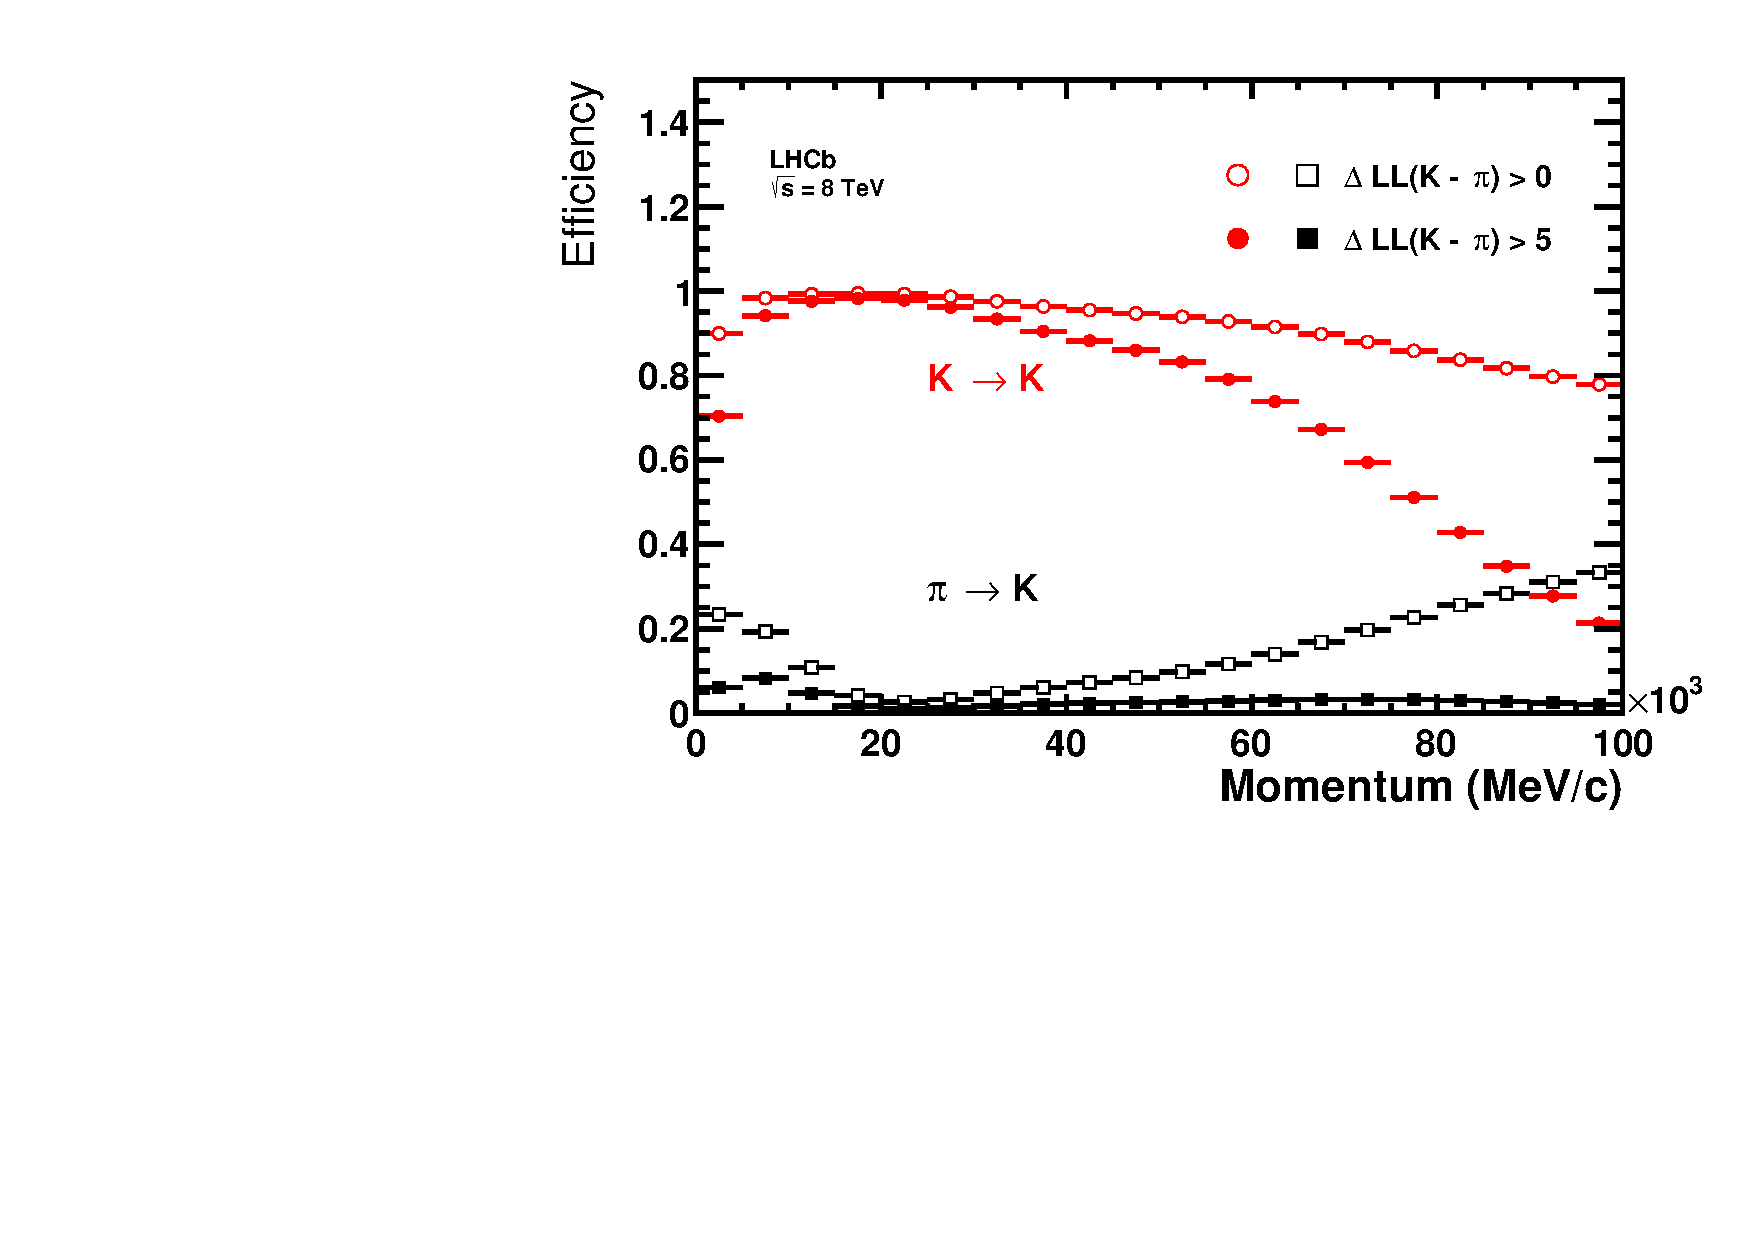
\includegraphics[width=1.0\textwidth]{figs/Detector/rich_k_pi_2012.pdf}
        \caption{2012}
    \end{subfigure}
    \begin{subfigure}[t]{0.4\textwidth}
        \centering
        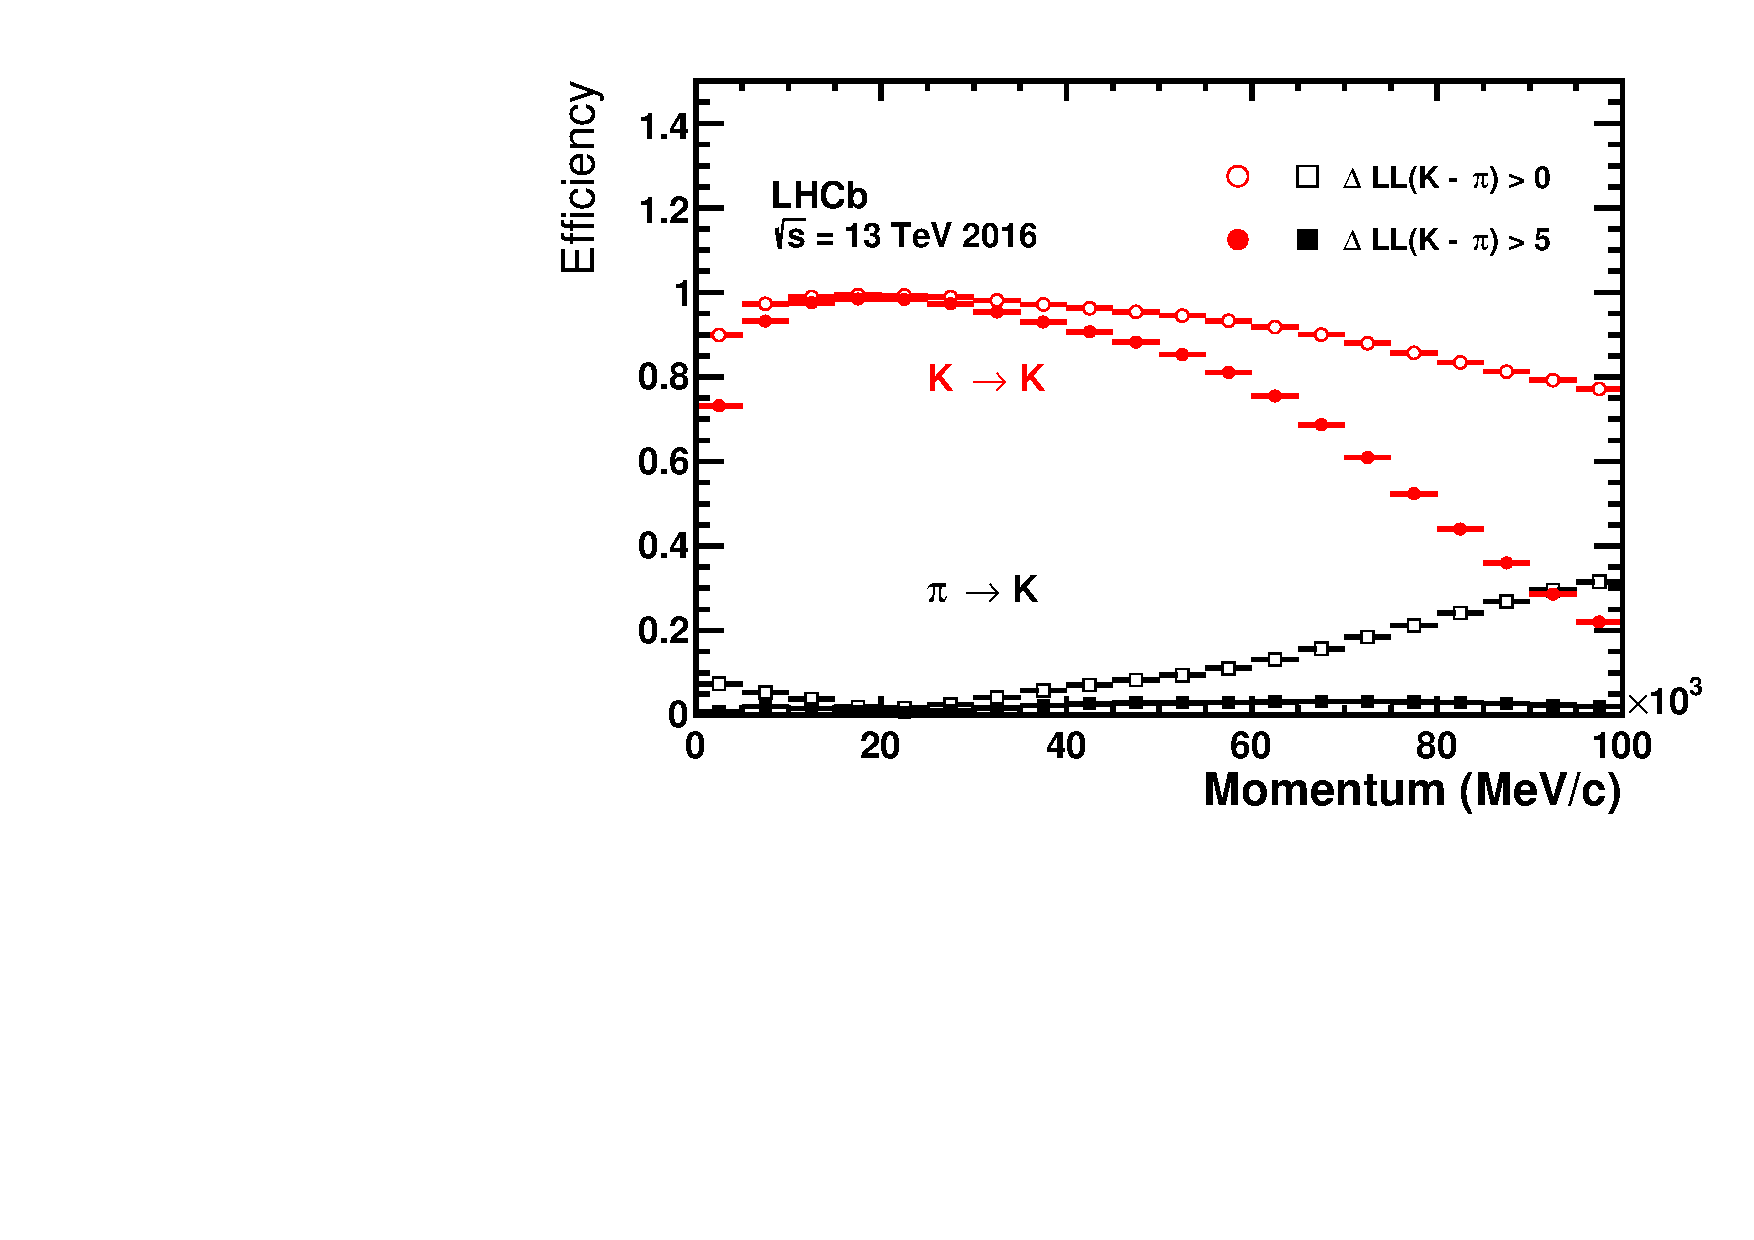
\includegraphics[width=1.0\textwidth]{figs/Detector/rich_k_pi_2016.pdf}
        \caption{2016}
    \end{subfigure}
    \caption{The \rich detector performance for kaon and pion separation, from Ref.~\cite{LHCb-DP-2012-003}.}
    \label{fig:Dec_rich_k_pi}   
\end{figure}
%%%%%%%%%%%%%%%%%%%%%%%%%%%%%%%%%%%%%%%%%%%%%%%%%%%%%%%%%%


\subsection{Calorimeters}

The calorimetry system is made of four components described below: the scintillator pad detector (\spd), pre-shower detector (\presh), electromagnetic calorimeter (\ecal) and the hadronic calorimeter (\hcal).
Primarily, these detectors measure energy deposited by particles. Such functionality is vital for neutral pions or photons that don't interact with the tracking stations. Critical to the triggering of \lhcb, the calorimeters provide fast identification of high transverse energy deposits that indicate hard proton-proton scatter. The four components work together to improve the discrimination of different particle species, in particular between electrons and hadrons. 



All of the calorimeter components work on the same basic principle; the particles pass through a transparent materials producing a flash of scintillation light. This light is collected and the quantity is related to the energy deposited by the particle.  



%%%%%%%%%%%%%%%%%%%%%%%%%%%%%%%%%%%%%%%%%%%%%%%%%%%%%%%%%%
\begin{figure}[!h]
    \centering
    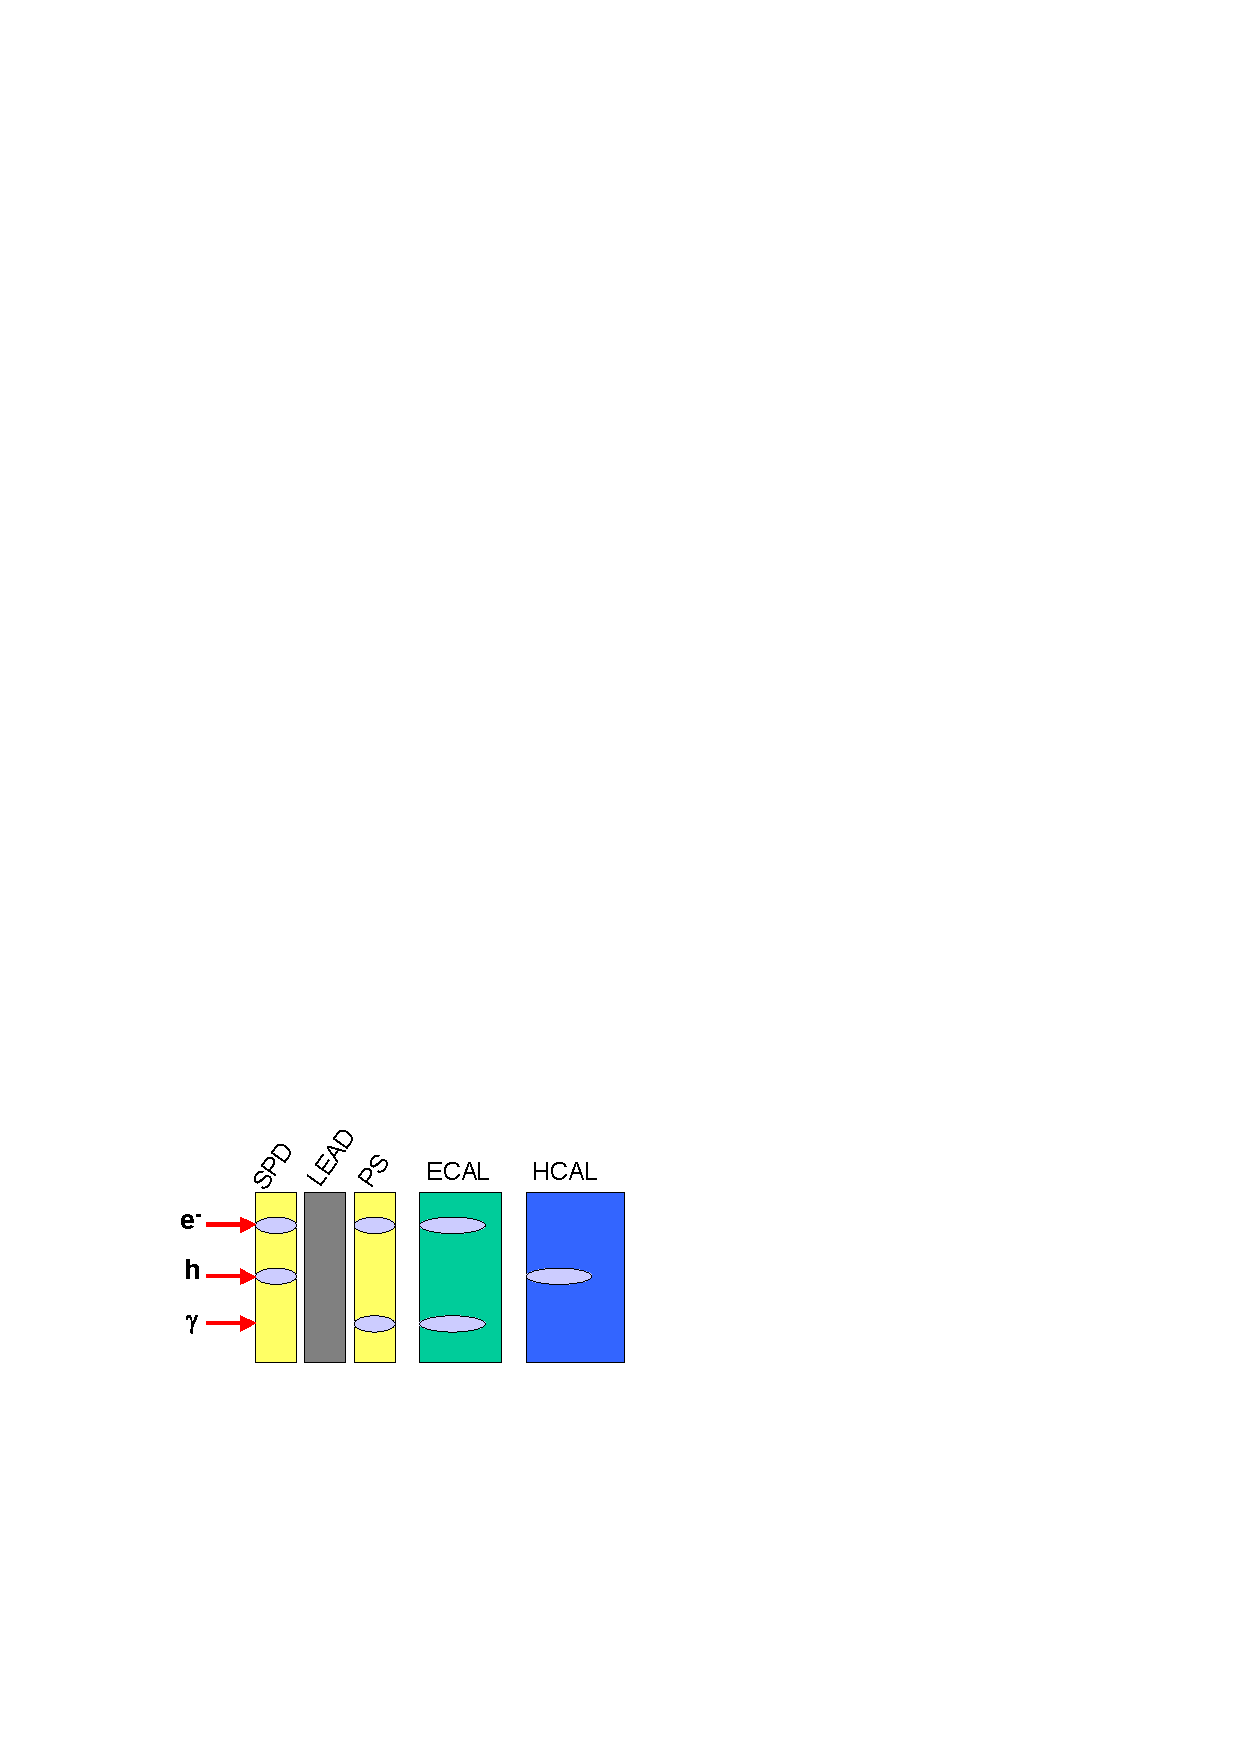
\includegraphics[width=0.6\textwidth]{figs/Detector/calo_layout.pdf}
    \caption{A diagram illustrating how the combined response of the calorimeter system aids particle identification, from Ref.~\cite{1742-6596-293-1-012059}.}
    \label{fig:Dec_calo_layout}   
\end{figure}
%%%%%%%%%%%%%%%%%%%%%%%%%%%%%%%%%%%%%%%%%%%%%%%%%%%%%%%%%%


The first layer of the calorimeter system is the scintillator pad detector (\spd), as shown in Fig.~\ref{fig:Dec_calo_layout}. This provides information about whether the incident particles are neutral or charged. After this comes the pre-shower detector (\presh). This indicates the electromagnetic nature of the of the particle. For charged particles this separates electrons and charged hadrons; for neutral particle it helps separate photons from neutral hadrons. Next comes the electromagnetic calorimeter (\ecal) tasked with measuring the energy of electromagnetically interacting particles, including electrons and photons. Finally, the hadronic calorimeter (\hcal) determines the energy deposited by hadrons, including pions, kaons, protons and neutrons. 

\subsubsection{Scintillator pad detector and Pre-shower detector}

The \spd and \presh are almost identical scintillating pads detectors constructed from a mix of polystyrene and wavelength-shifting dopants. The pads are coated in light-proof paper and contain loops of wavelength-shifting fibres to collect the scintillation light. The pads are segmented into cells, matching the granularity of the \ecal detector.
The fibres are connected to long clear fibres connected to photo-multiplier tubes (PMT) outside the detectors acceptance. Between the \spd and \presh detectors is a 15\mm thick layer of lead. This dense layer initiates electrons and photons to shower electromagnetically, depositing some of their energy in the \presh scintillating pads.    


\subsubsection{Electronic Calorimeter}


The \ecal is made of 66 layers of alternating lead and scintillator, with a total depth of 42\cm. This thickness corresponds to 25 radiation lengths. The layout of the layers are shown in Fig.~\ref{fig:Dec_ecal_layout}. Scintillating light is captured and transported by wavelength-shifting wires that pass through the entire structure. The light is measured by PMTs positioned at the end of the structure. The cells of the \ecal are segmented differently depending on the proximity to the beam-pipe, as shown in Fig.~\ref{fig:Dec_ecal_layout}. The cells are split into inner, middle and outer regions with sizes $4\times 4\cm$, $6\times 6\cm$ and $12\times 12\cm$ respectively. 

%%%%%%%%%%%%%%%%%%%%%%%%%%%%%%%%%%%%%%%%%%%%%%%%%%%%%%%%%%
\begin{figure}[!h]
    \centering
    \begin{subfigure}[m]{0.4\textwidth}
        \centering        
        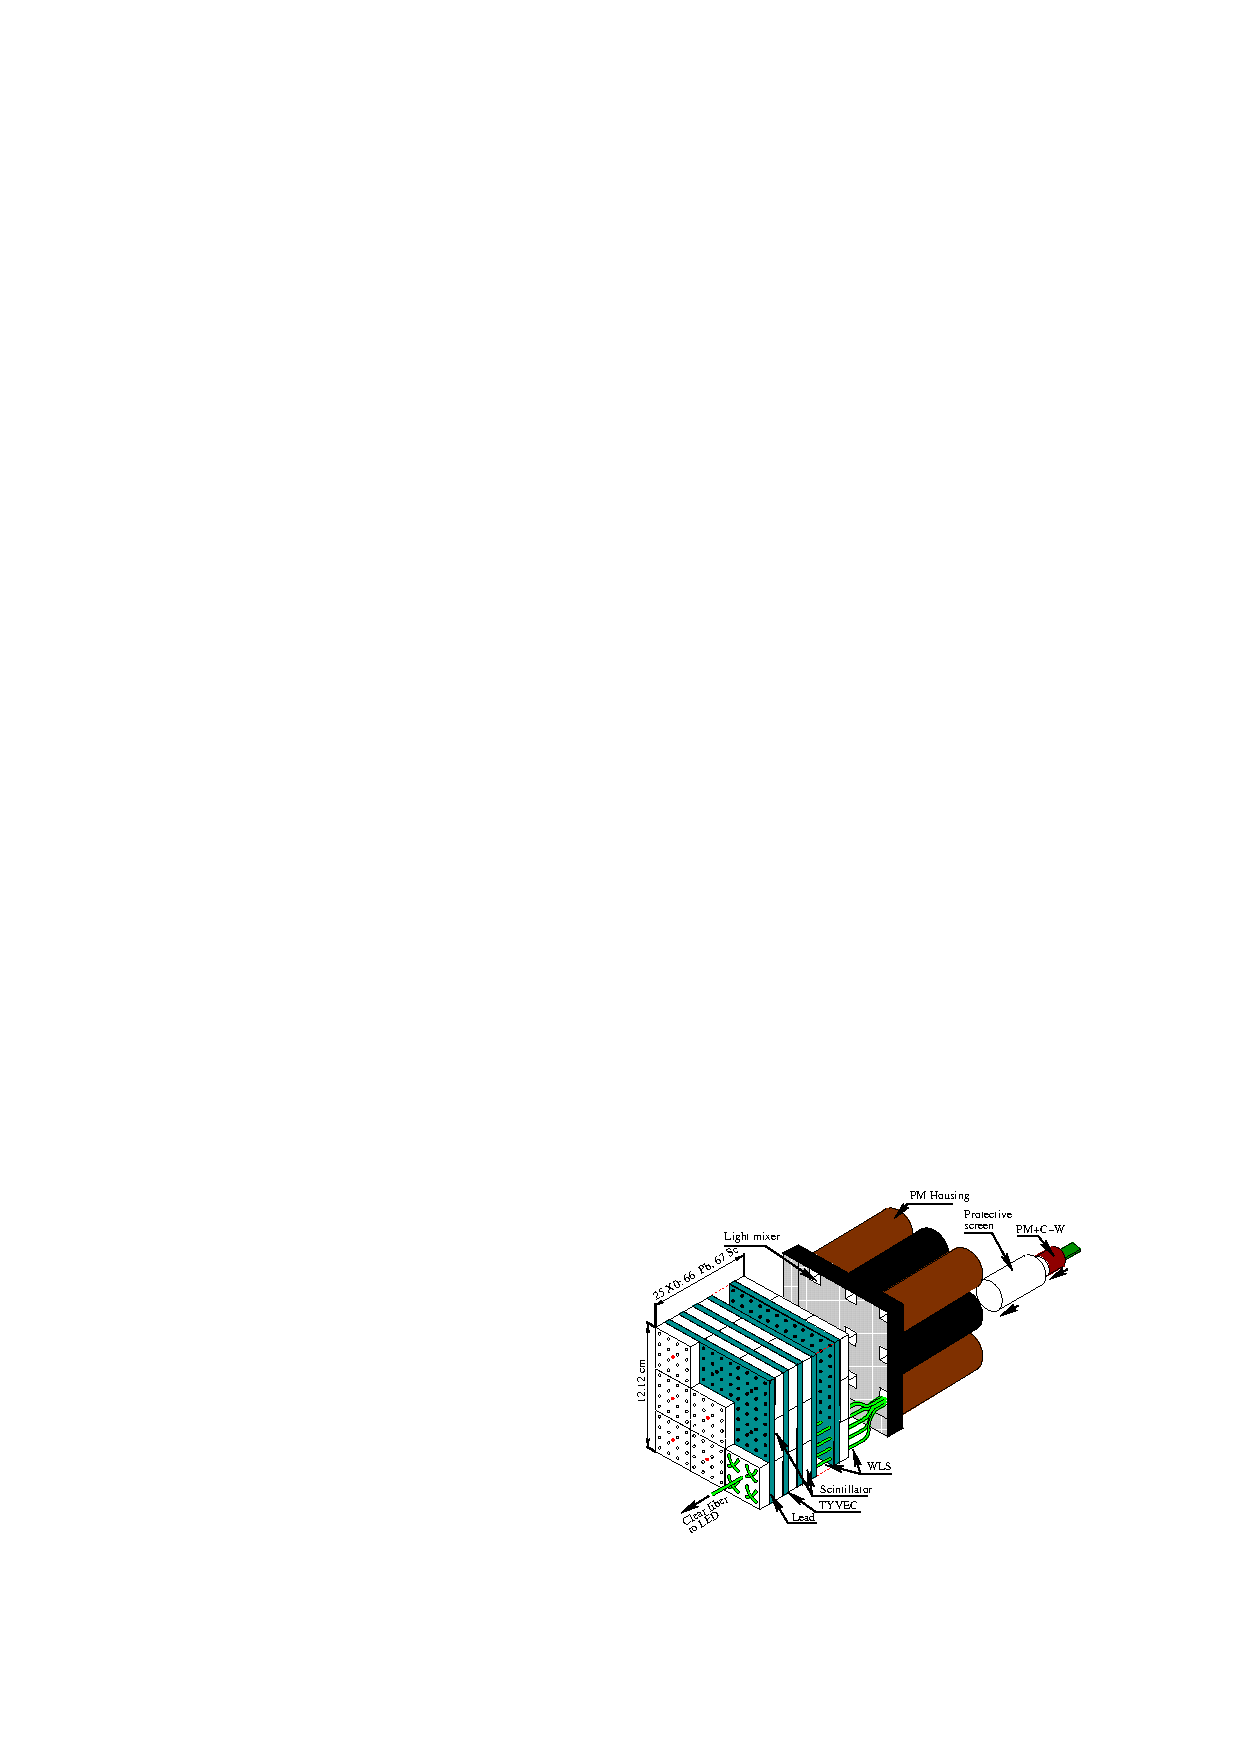
\includegraphics[width=1.0\textwidth]{figs/Detector/ecal_diagram.pdf}
    \end{subfigure}
    \begin{subfigure}[m]{0.4\textwidth}
        \centering
        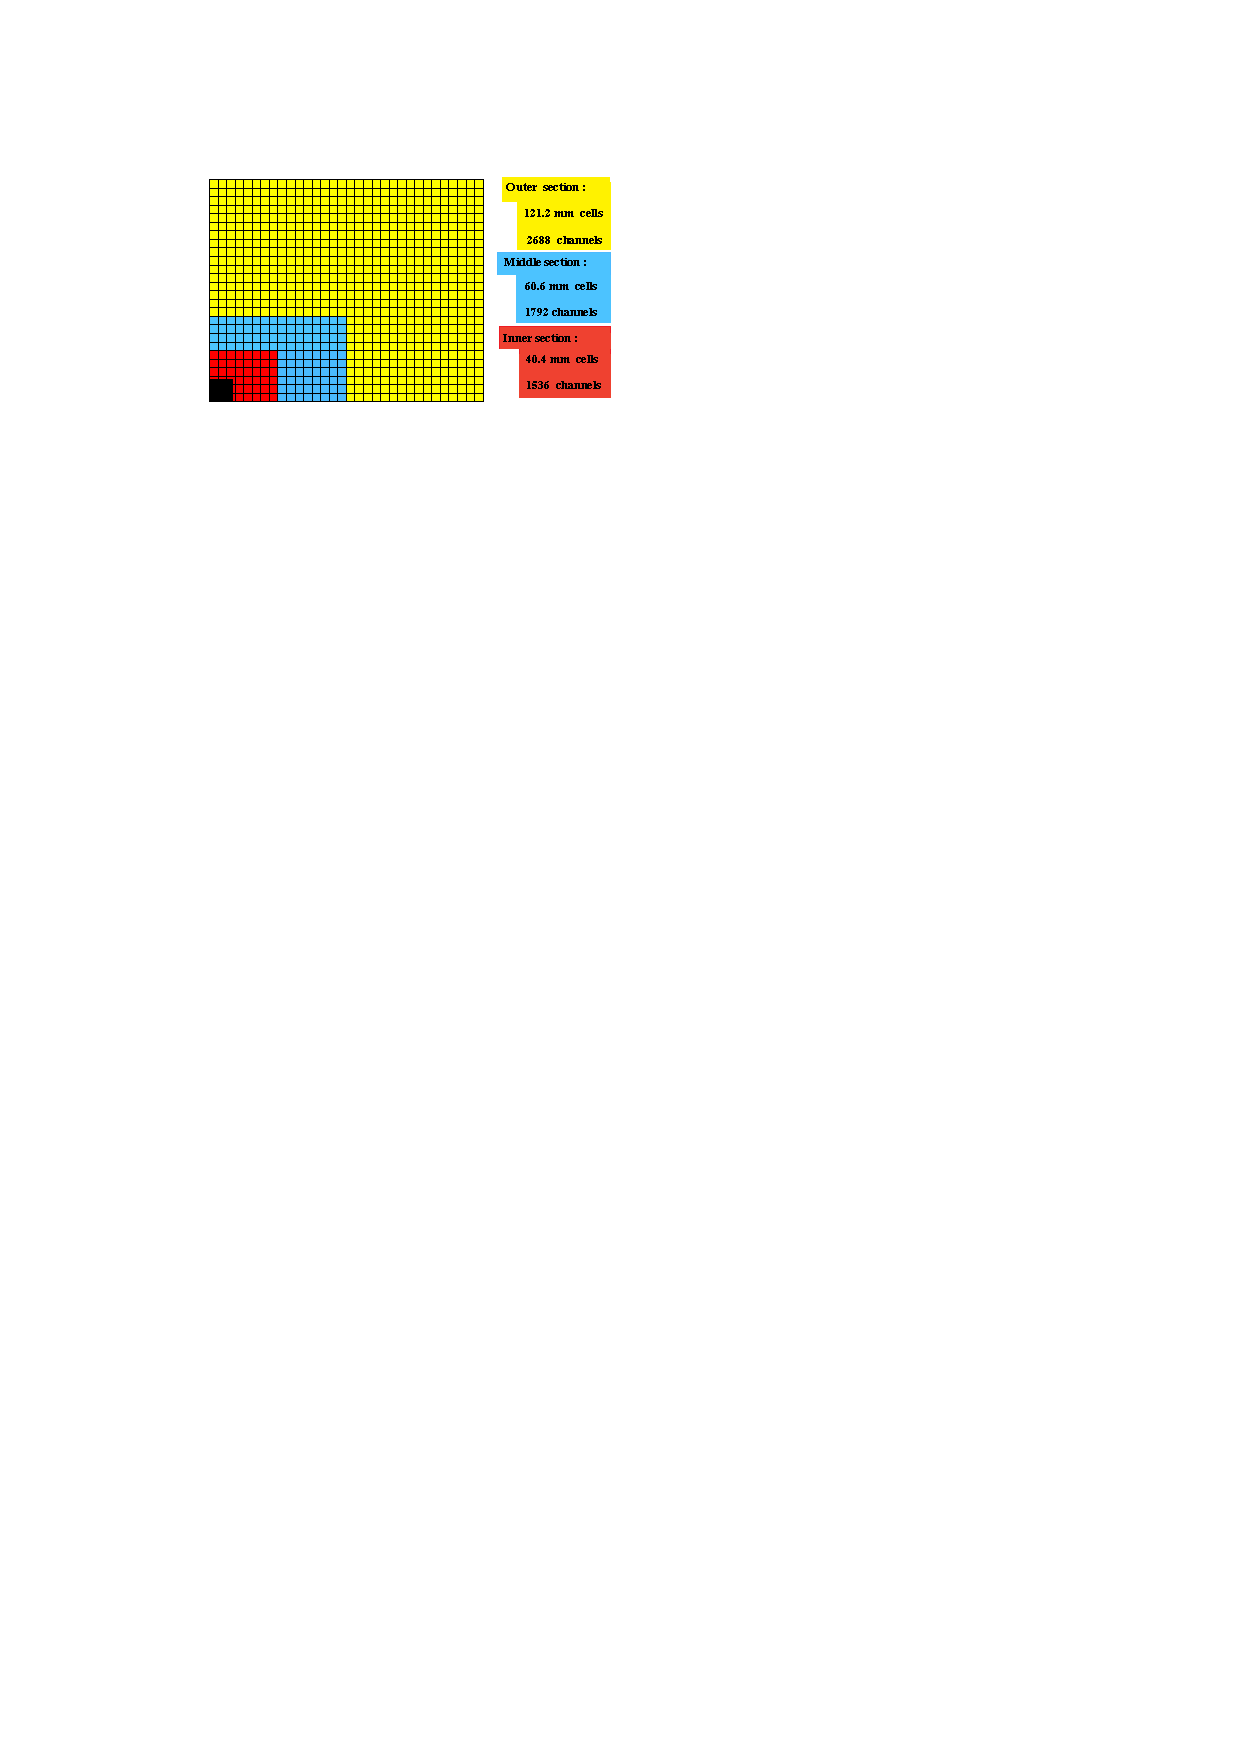
\includegraphics[width=1.0\textwidth]{figs/Detector/ecal_layout.pdf}
    \end{subfigure}
    \caption{A diagram of one of the inner \ecal modules (left) and the layout of one quarter of the \ecal modules (right), from Ref.~\cite{Alves:2008zz} and Ref.~\cite{doi:1765047}.}
    \label{fig:Dec_ecal_layout}   
\end{figure}
%%%%%%%%%%%%%%%%%%%%%%%%%%%%%%%%%%%%%%%%%%%%%%%%%%%%%%%%%%

The resolution of the \ecal in Run I can be parametrised as 
\begin{equation}
\frac{\sigma_{E}}{E} = \frac{(8.5-9.5)\%}{\sqrt{E}} \oplus 0.8\%,
\end{equation}
where the energy $E$ is measured in \gev (from Ref.~\cite{1748-0221-12-07-C07024}). During data taking the \ecal receives a large dose of radiation. This radiation damages the detector modules as well as the light guides and PMTs. The measurement of irradiation can be quantified by looking at the PMT light yields, as shown in Fig.~\ref{fig:Dec_calo_damage}. This can be extrapolated to determine if the innermost \ecal modules will remain operational for a total data set corresponding to an integrated luminosity of 13--16\invfb ($\int_{2010}^{2018}\mathcal{L} \approx 9 \invfb $).   


%%%%%%%%%%%%%%%%%%%%%%%%%%%%%%%%%%%%%%%%%%%%%%%%%%%%%%%%%%
\begin{figure}[!h]
    \centering        
    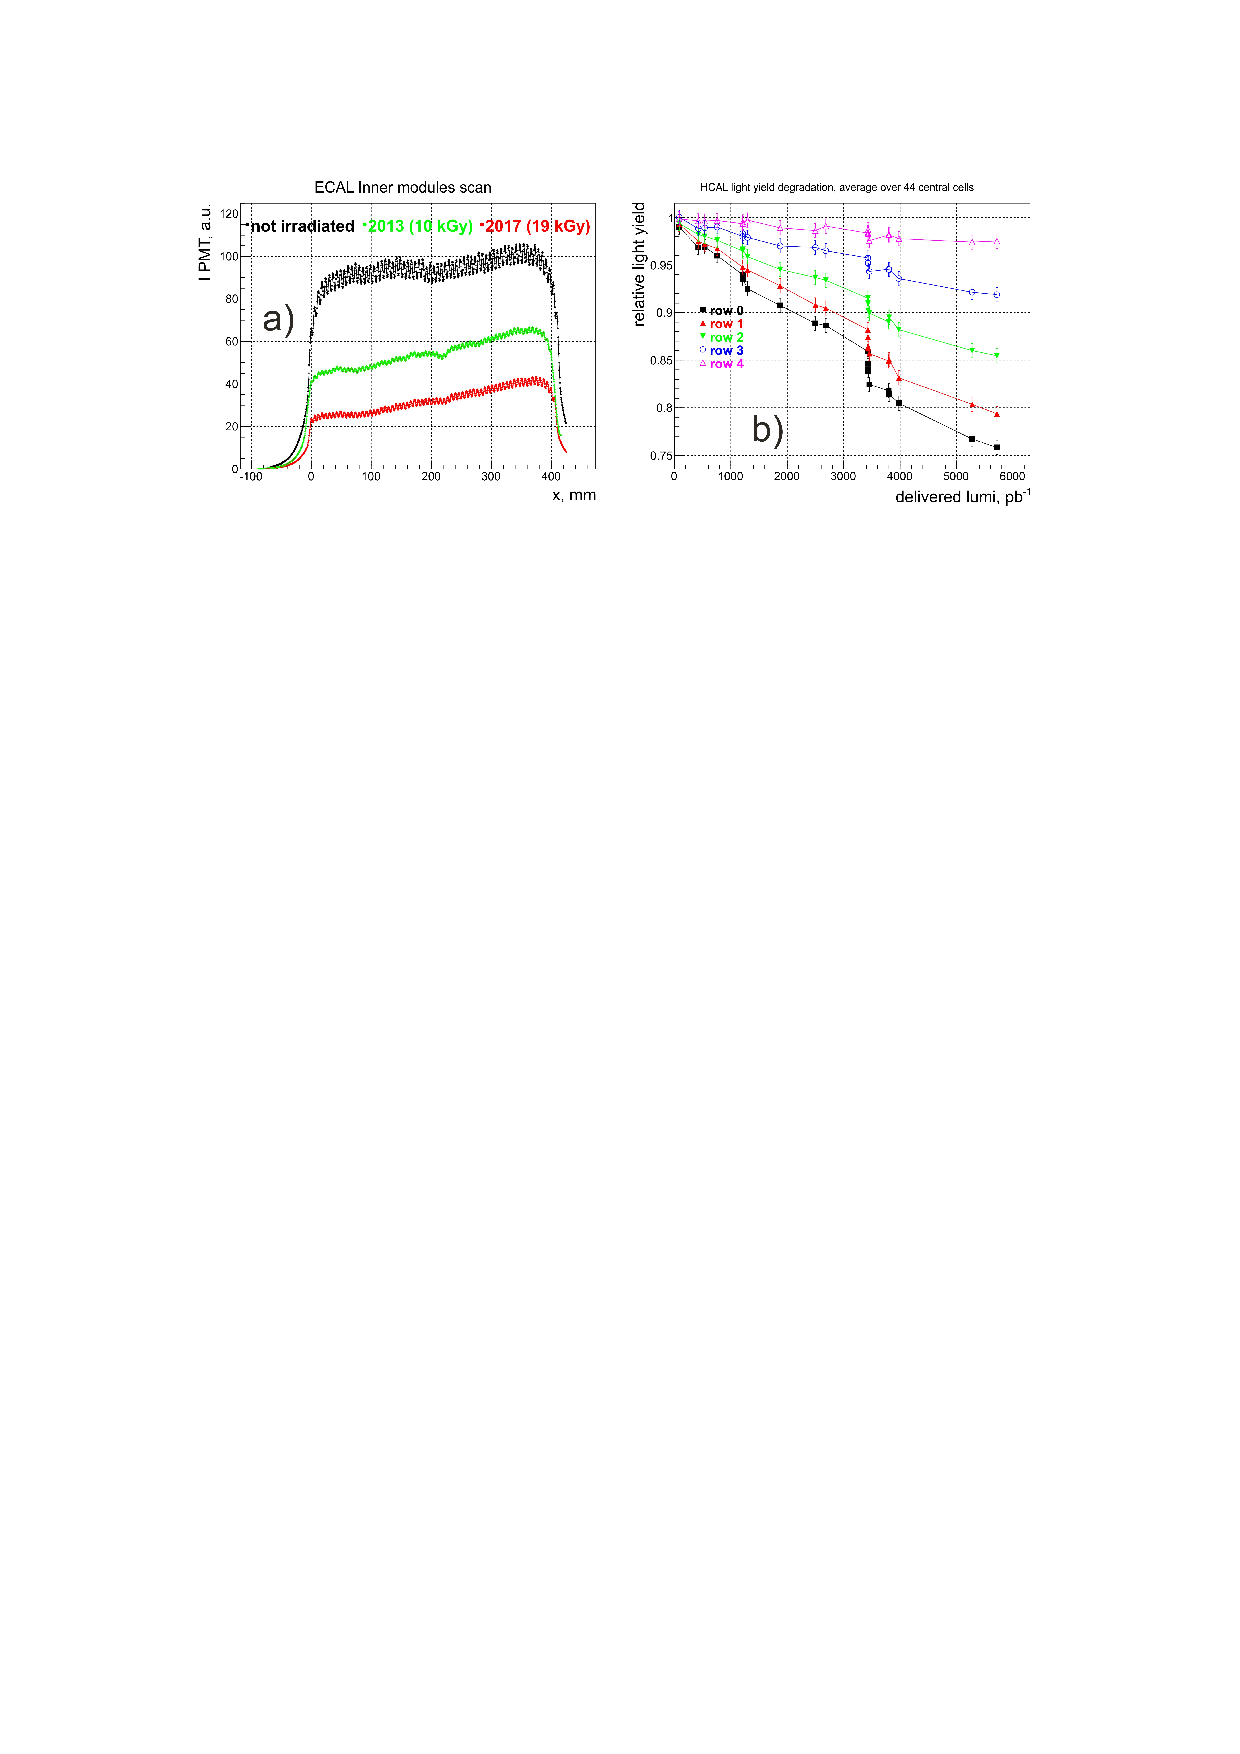
\includegraphics[width=1.0\textwidth]{figs/Detector/calo_performance.pdf}
    \caption{The result of radiation damage to the \ecal (a) and \hcal detectors (b), from Ref.~\cite{1748-0221-12-07-C07024}.}
    \label{fig:Dec_calo_damage}   
\end{figure}
%%%%%%%%%%%%%%%%%%%%%%%%%%%%%%%%%%%%%%%%%%%%%%%%%%%%%%%%%%

\subsubsection{Hadronic calorimeter}

The \hcal is a 500 tonne detector constructed from iron plates and scintillating tiles. Unlike the \ecal, these are arranged parallel to the beam-pipe as shown in Fig.~\ref{fig:Dec_hcal_layout}. The cells vary in size in the different regions of the detector; the inner regions correspond to $13 \times 13 \cm$ cells and the outer to $26\times26\cm$. The widths of the iron tiles are chosen to be one radiation length (1\cm), and the lengths are one hadron interaction length. The scintillation light is collected by wavelength-shifting fibres that are read out by PMTs located at the rear of each cell.    


%%%%%%%%%%%%%%%%%%%%%%%%%%%%%%%%%%%%%%%%%%%%%%%%%%%%%%%%%%
\begin{figure}[!h]
    \centering
    \begin{subfigure}[m]{0.4\textwidth}
        \centering        
        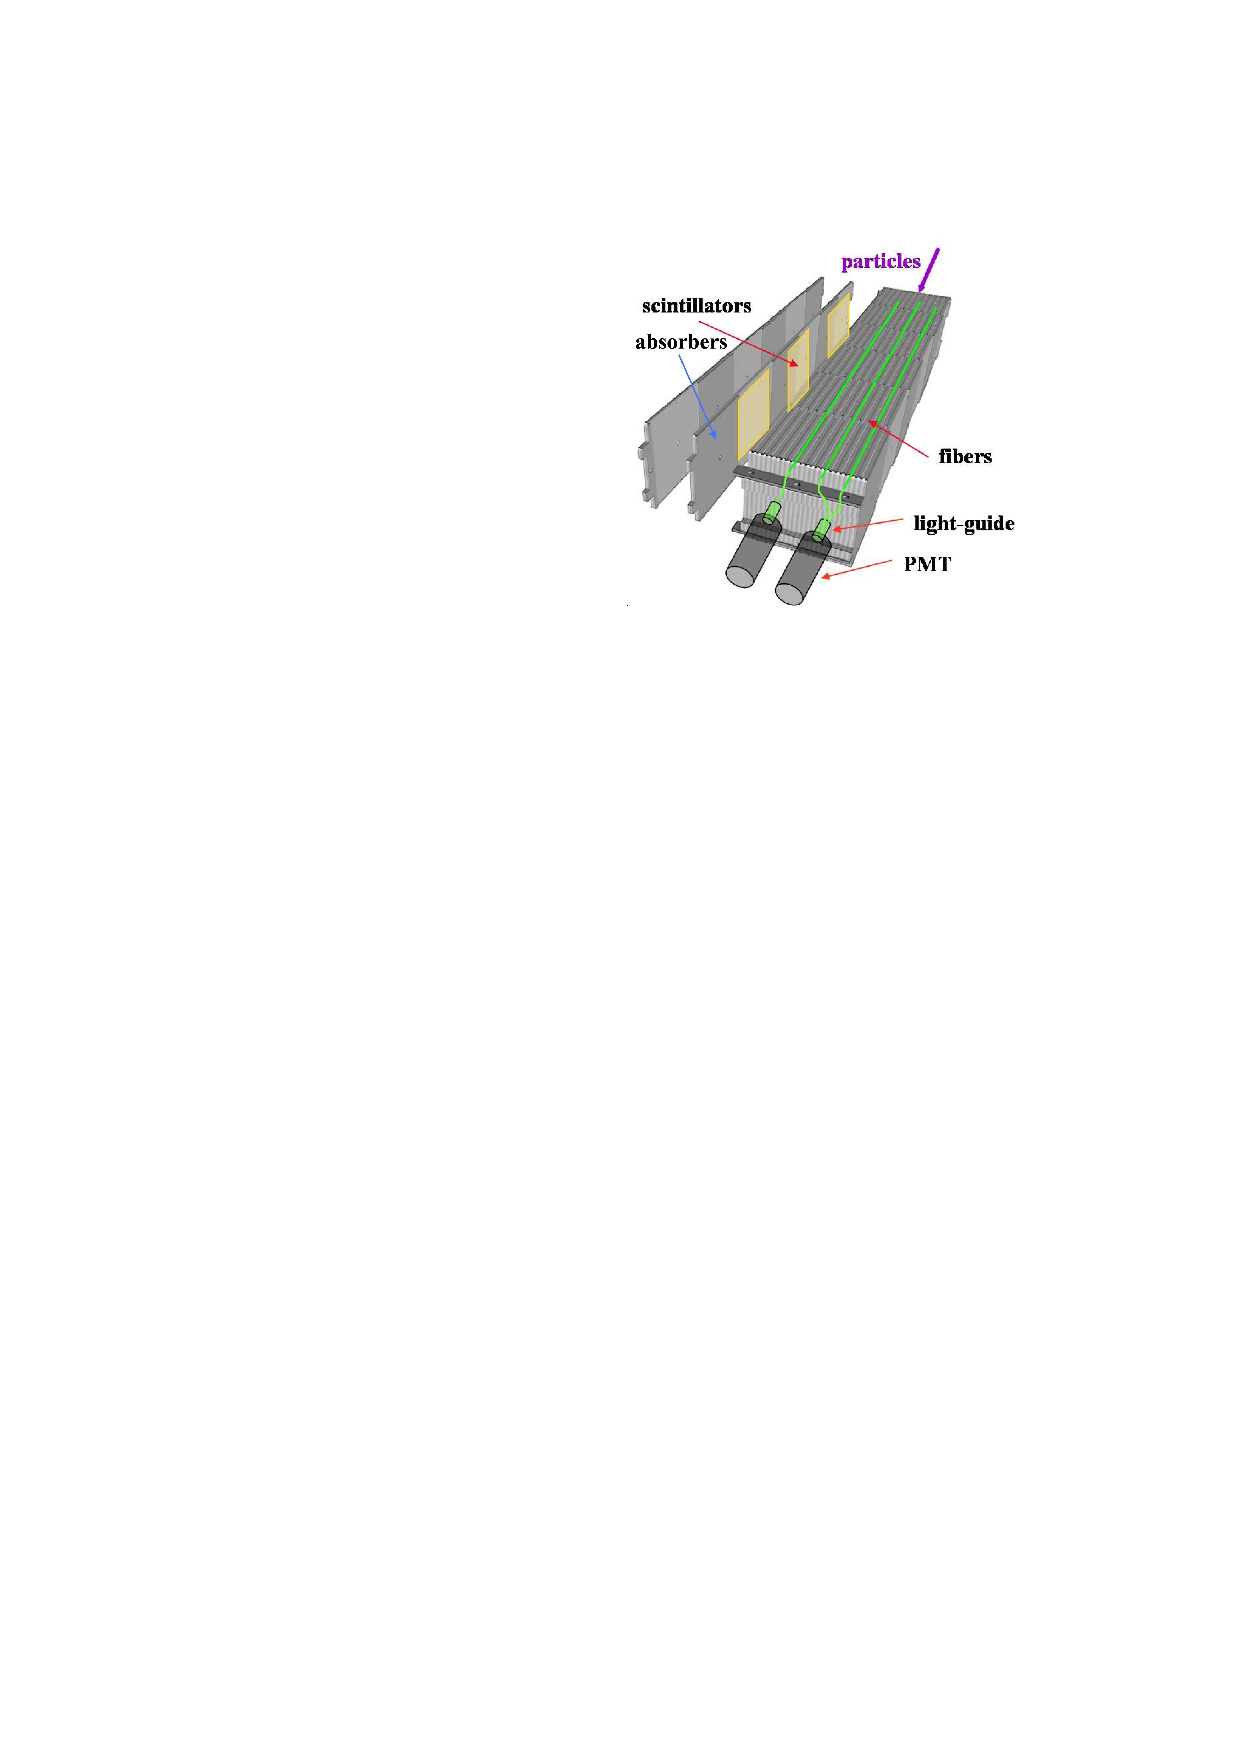
\includegraphics[width=1.0\textwidth]{figs/Detector/hcal_diagram.pdf}
    \end{subfigure}
    \begin{subfigure}[m]{0.4\textwidth}
        \centering
        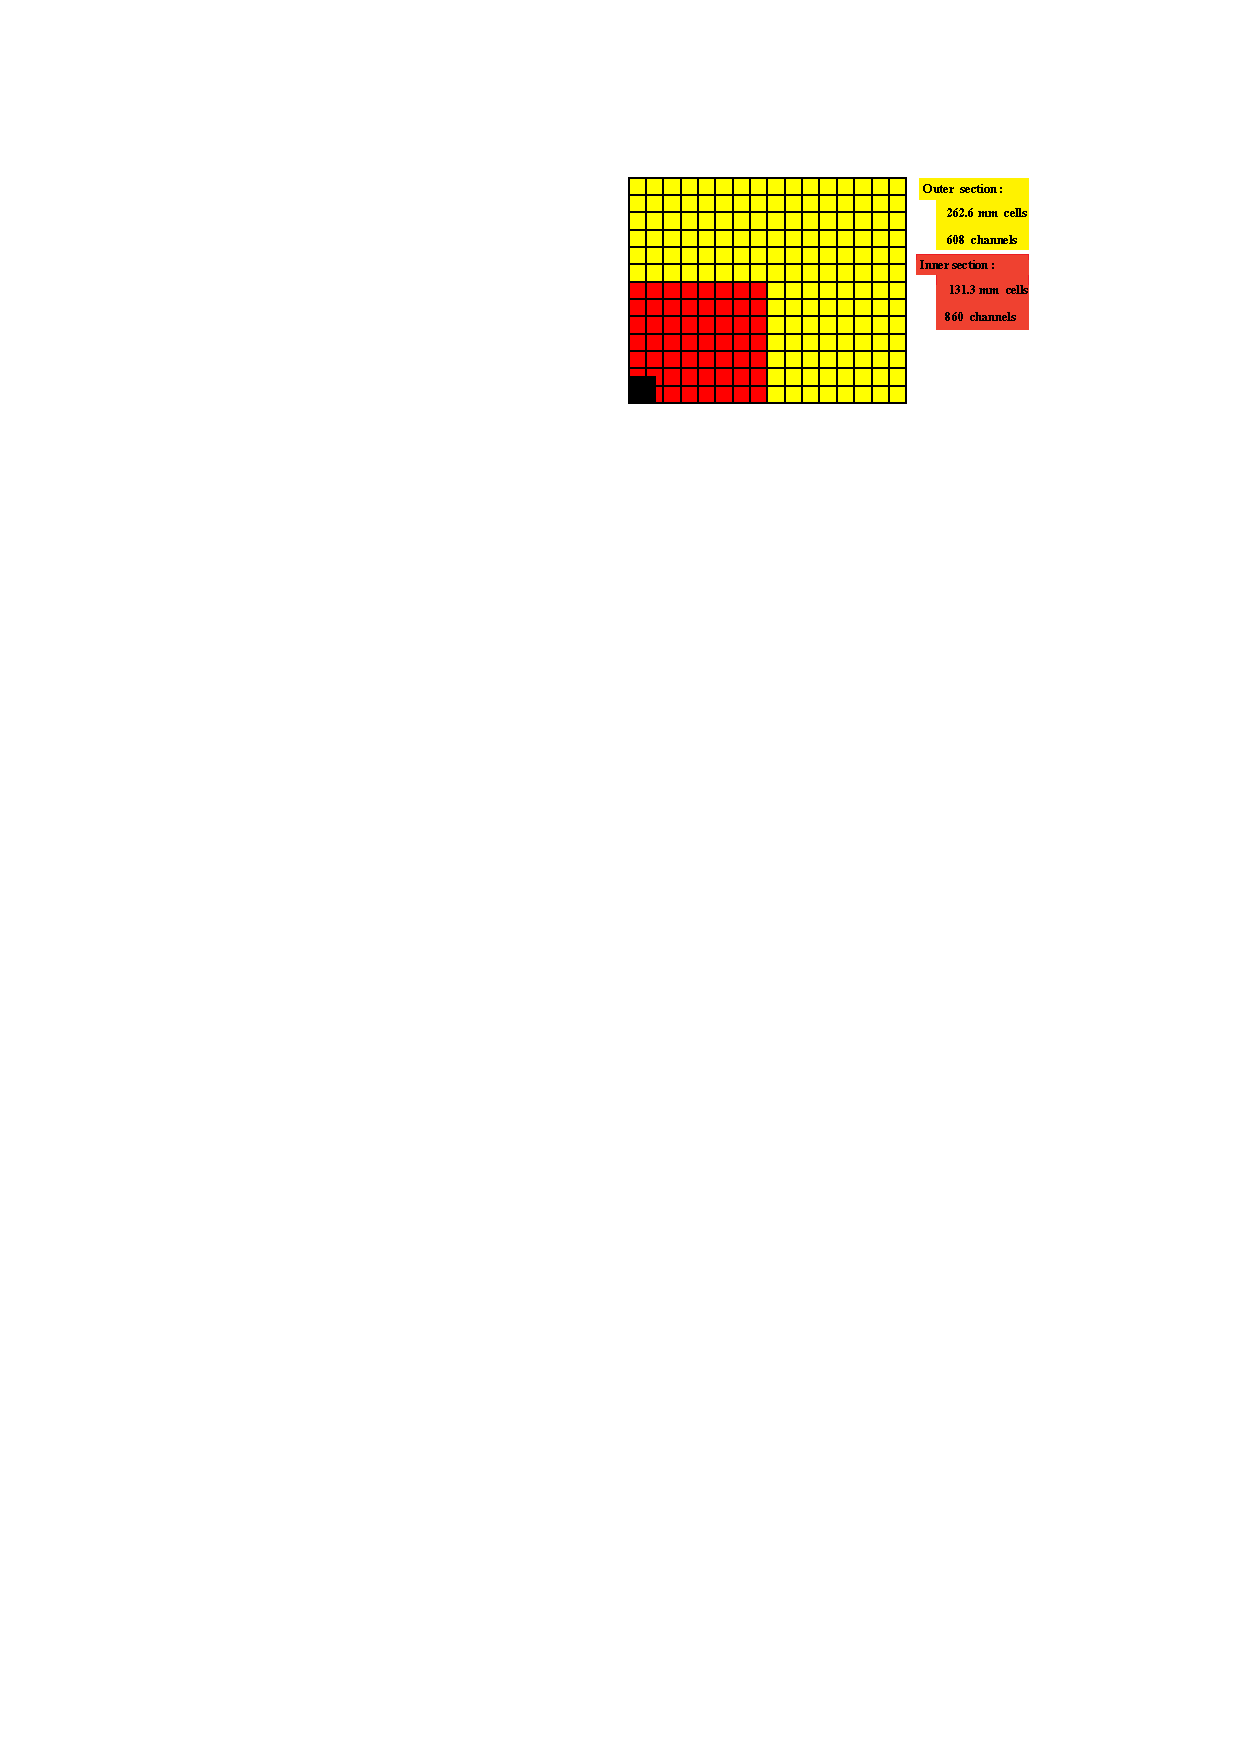
\includegraphics[width=1.0\textwidth]{figs/Detector/hcal_layout.pdf}
    \end{subfigure}
    \caption{A diagram of one of the \hcal modules (left) and the layout of one quarter of the \hcal modules (right), from Ref.~\cite{Alves:2008zz}.}
    \label{fig:Dec_hcal_layout}   
\end{figure}
%%%%%%%%%%%%%%%%%%%%%%%%%%%%%%%%%%%%%%%%%%%%%%%%%%%%%%%%%%


The Run I resolution of the \hcal can be parametrised as 
\begin{equation}
\frac{\sigma_{E}}{E} = \frac{(69\pm5)\%}{\sqrt{E}} \oplus (9\pm2)\%,
\end{equation}
where the energy $E$ is measured in \gev (from Ref.~\cite{1748-0221-12-07-C07024}).
The \hcal receives a large dose of radiation during data taking. This mainly affects the detector modules as the PMTs are located further away from the beam. The decrease in the light yield as a function of the accumulated data set is shown in Fig.~\ref{fig:Dec_calo_damage}.


\subsection{Muon system}


The muon system serves two main purposes: to provide fast muon \pt measurements for use in the hardware trigger; and to provide muon identification information for use in the software trigger and offline analyses.
The muon system is made of five rectangular stations. The first (M1) is positioned before the calorimeters and the remaining (M2--M4) are positioned after, as shown in Fig.~\ref{fig:Dec_muon_schematic}. The latter stations alternate with 80\cm layers of iron absorbers. The muon system is the last sub-detector as muons are highly penetrating particles, travelling through more material than other species. The interleaving iron absorbers help to isolate muons, as other particles are stopped by these layers. 

% %%%%%%%%%%%%%%%%%%%%%%%%%%%%%%%%%%%%%%%%%%%%%%%%%%%%%%%%%%
% \begin{figure}[!h]
%     \centering
%     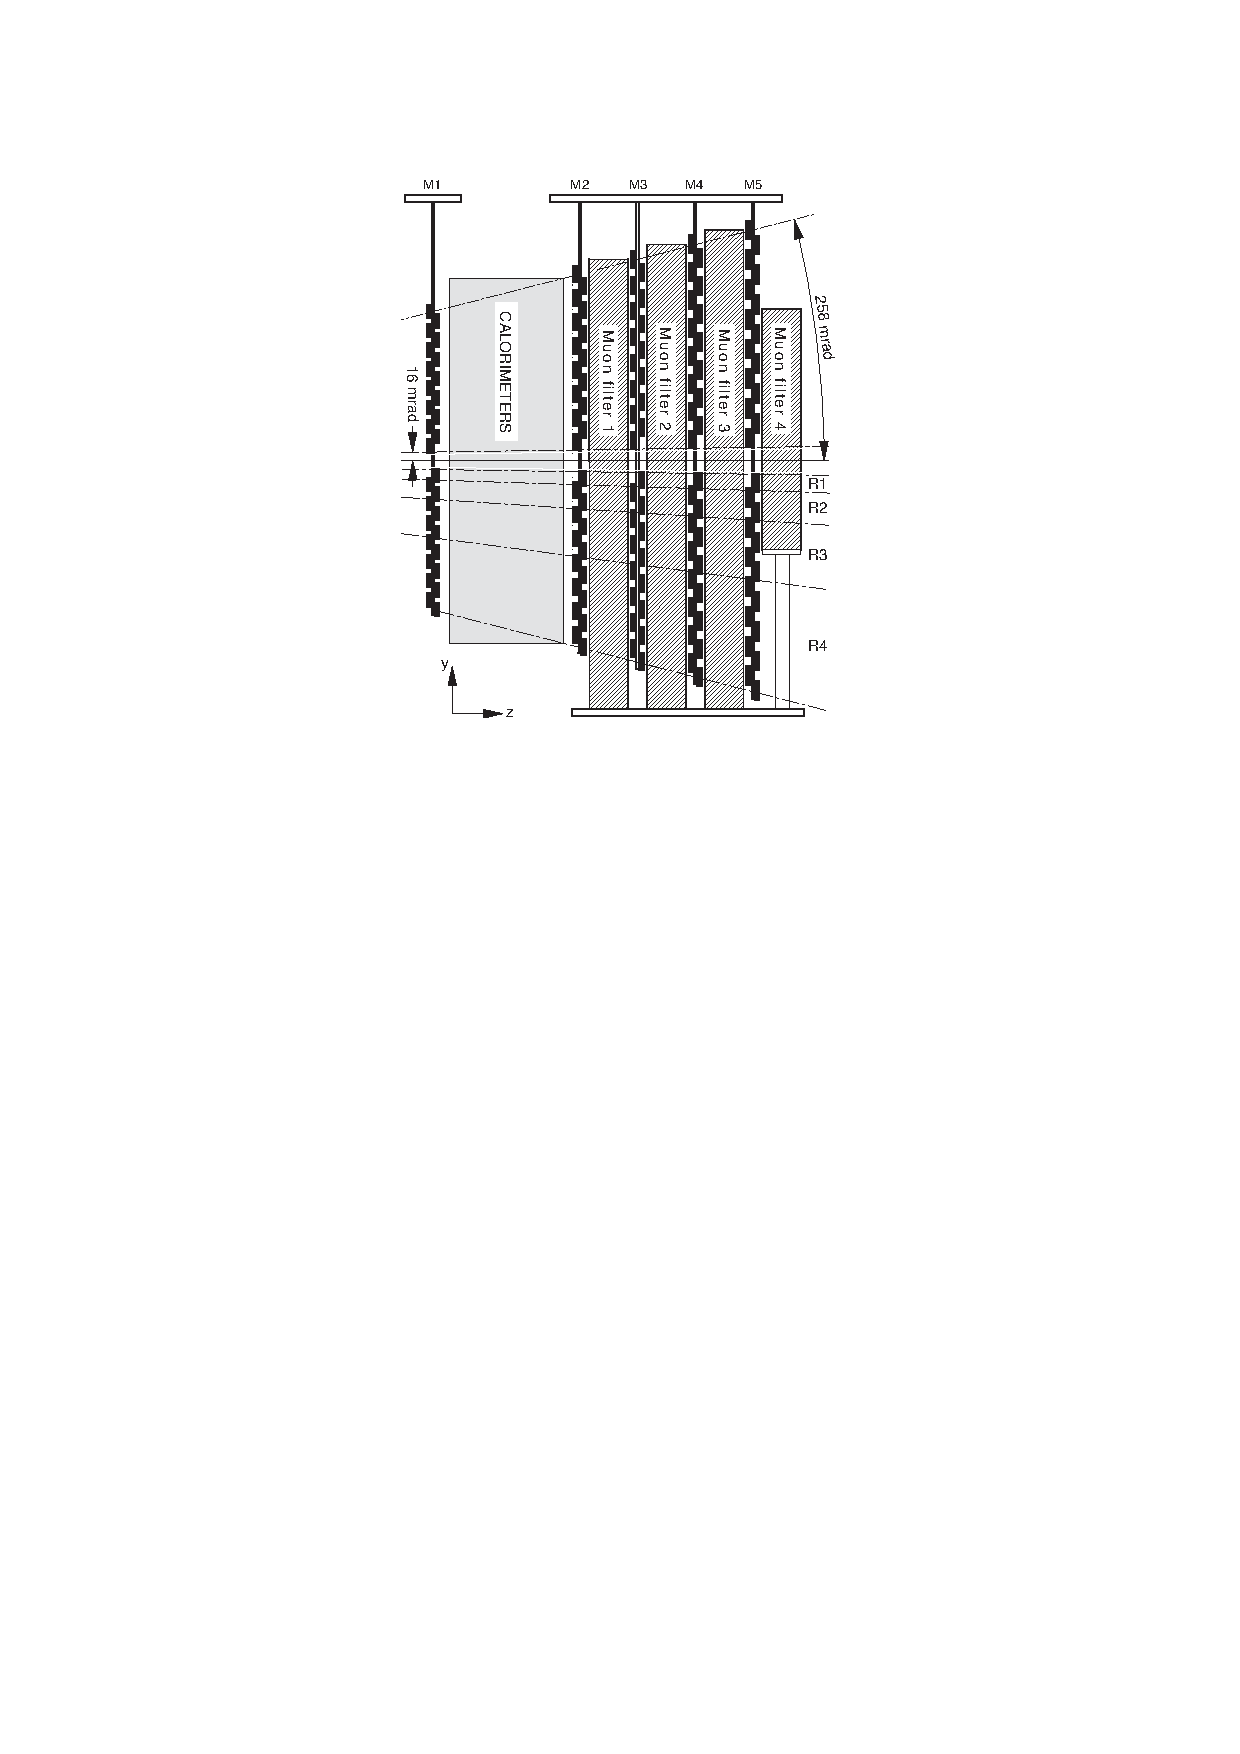
\includegraphics[width=0.4\textwidth]{figs/Detector/muon_layout.pdf}
%     \caption{Schematic of the Muon sub-detector, from Ref.~\cite{Alves:2008zz}.}
%     \label{fig:Dec_muon_schematic}   
% \end{figure}
% %%%%%%%%%%%%%%%%%%%%%%%%%%%%%%%%%%%%%%%%%%%%%%%%%%%%%%%%%%

%%%%%%%%%%%%%%%%%%%%%%%%%%%%%%%%%%%%%%%%%%%%%%%%%%%%%%%%%%
\begin{figure}[!h]
    \centering
    \begin{subfigure}[m]{0.4\textwidth}
        \centering        
        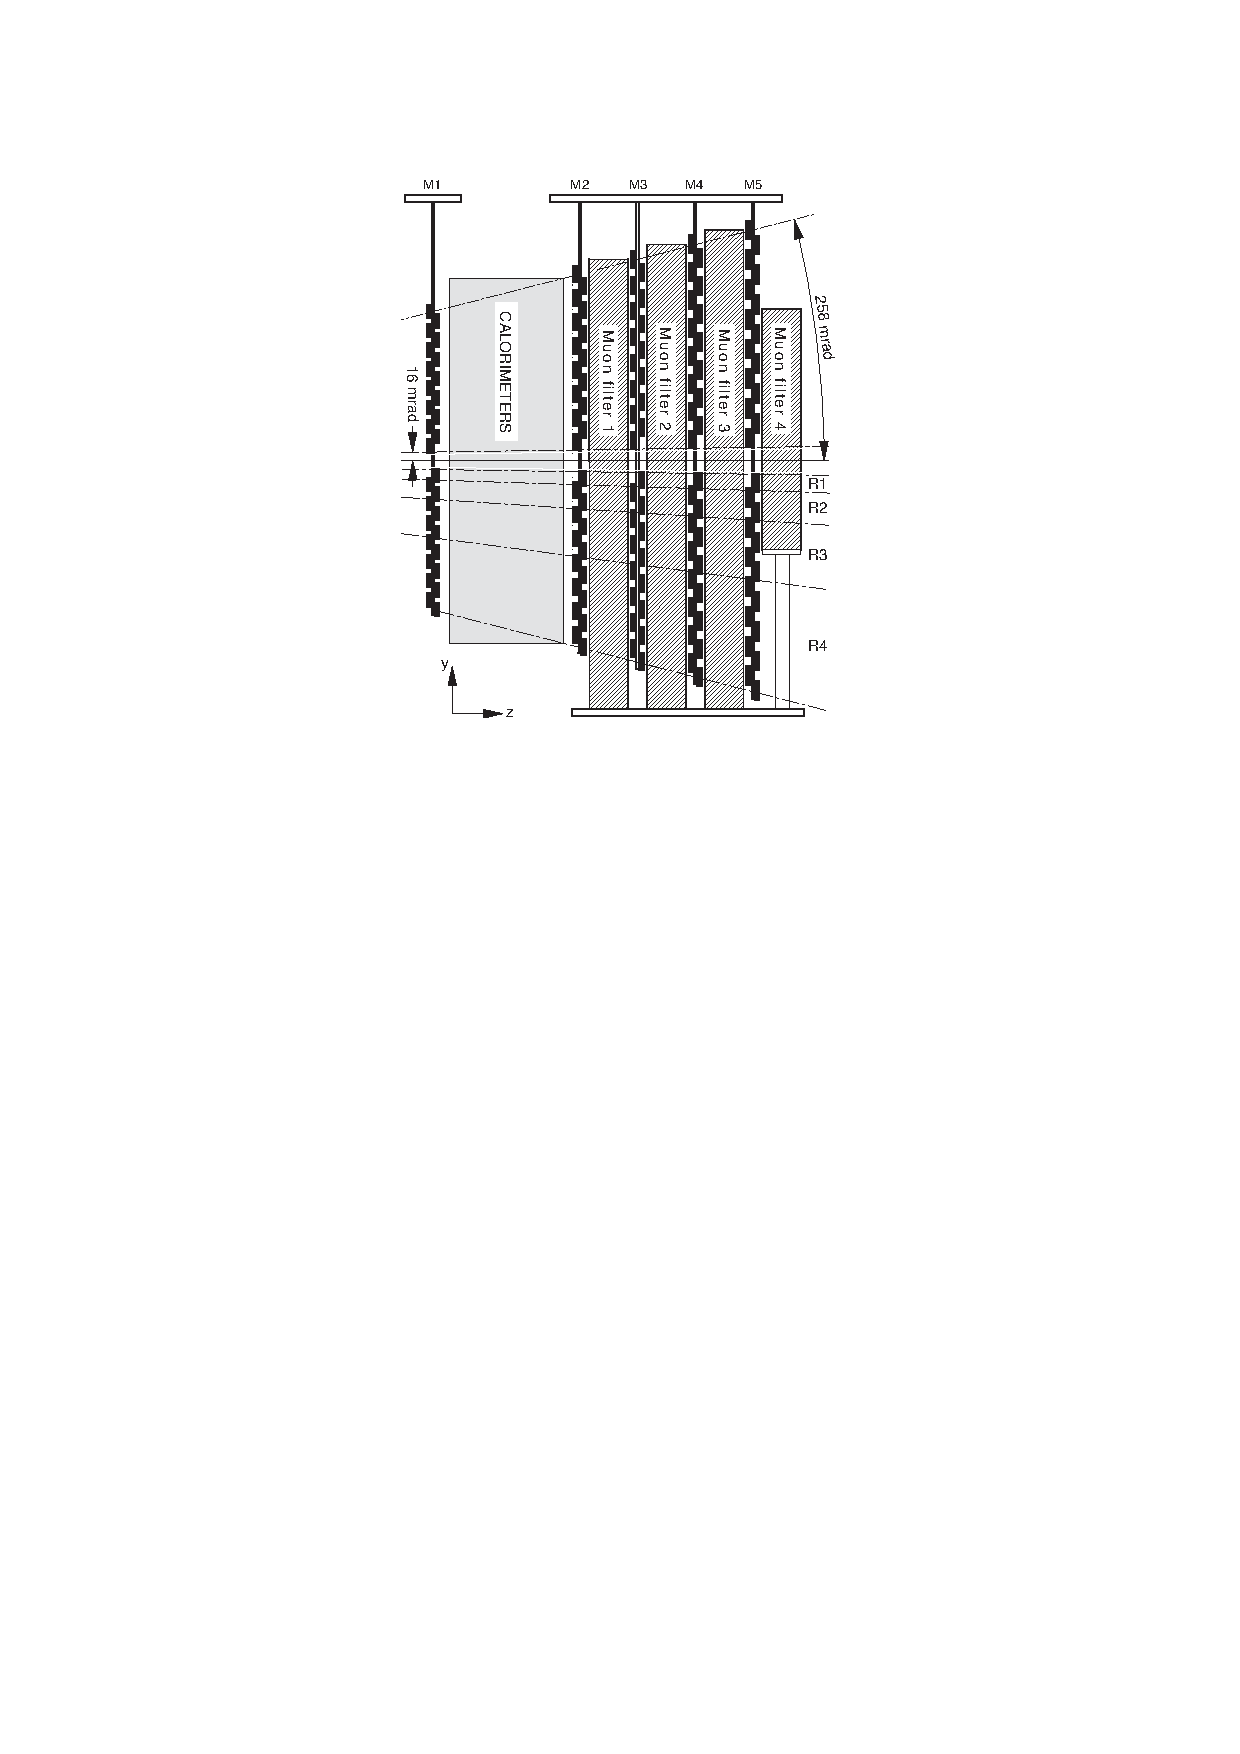
\includegraphics[width=1.0\textwidth]{figs/Detector/muon_layout.pdf}
    \end{subfigure}
    \begin{subfigure}[m]{0.4\textwidth}
        \centering
        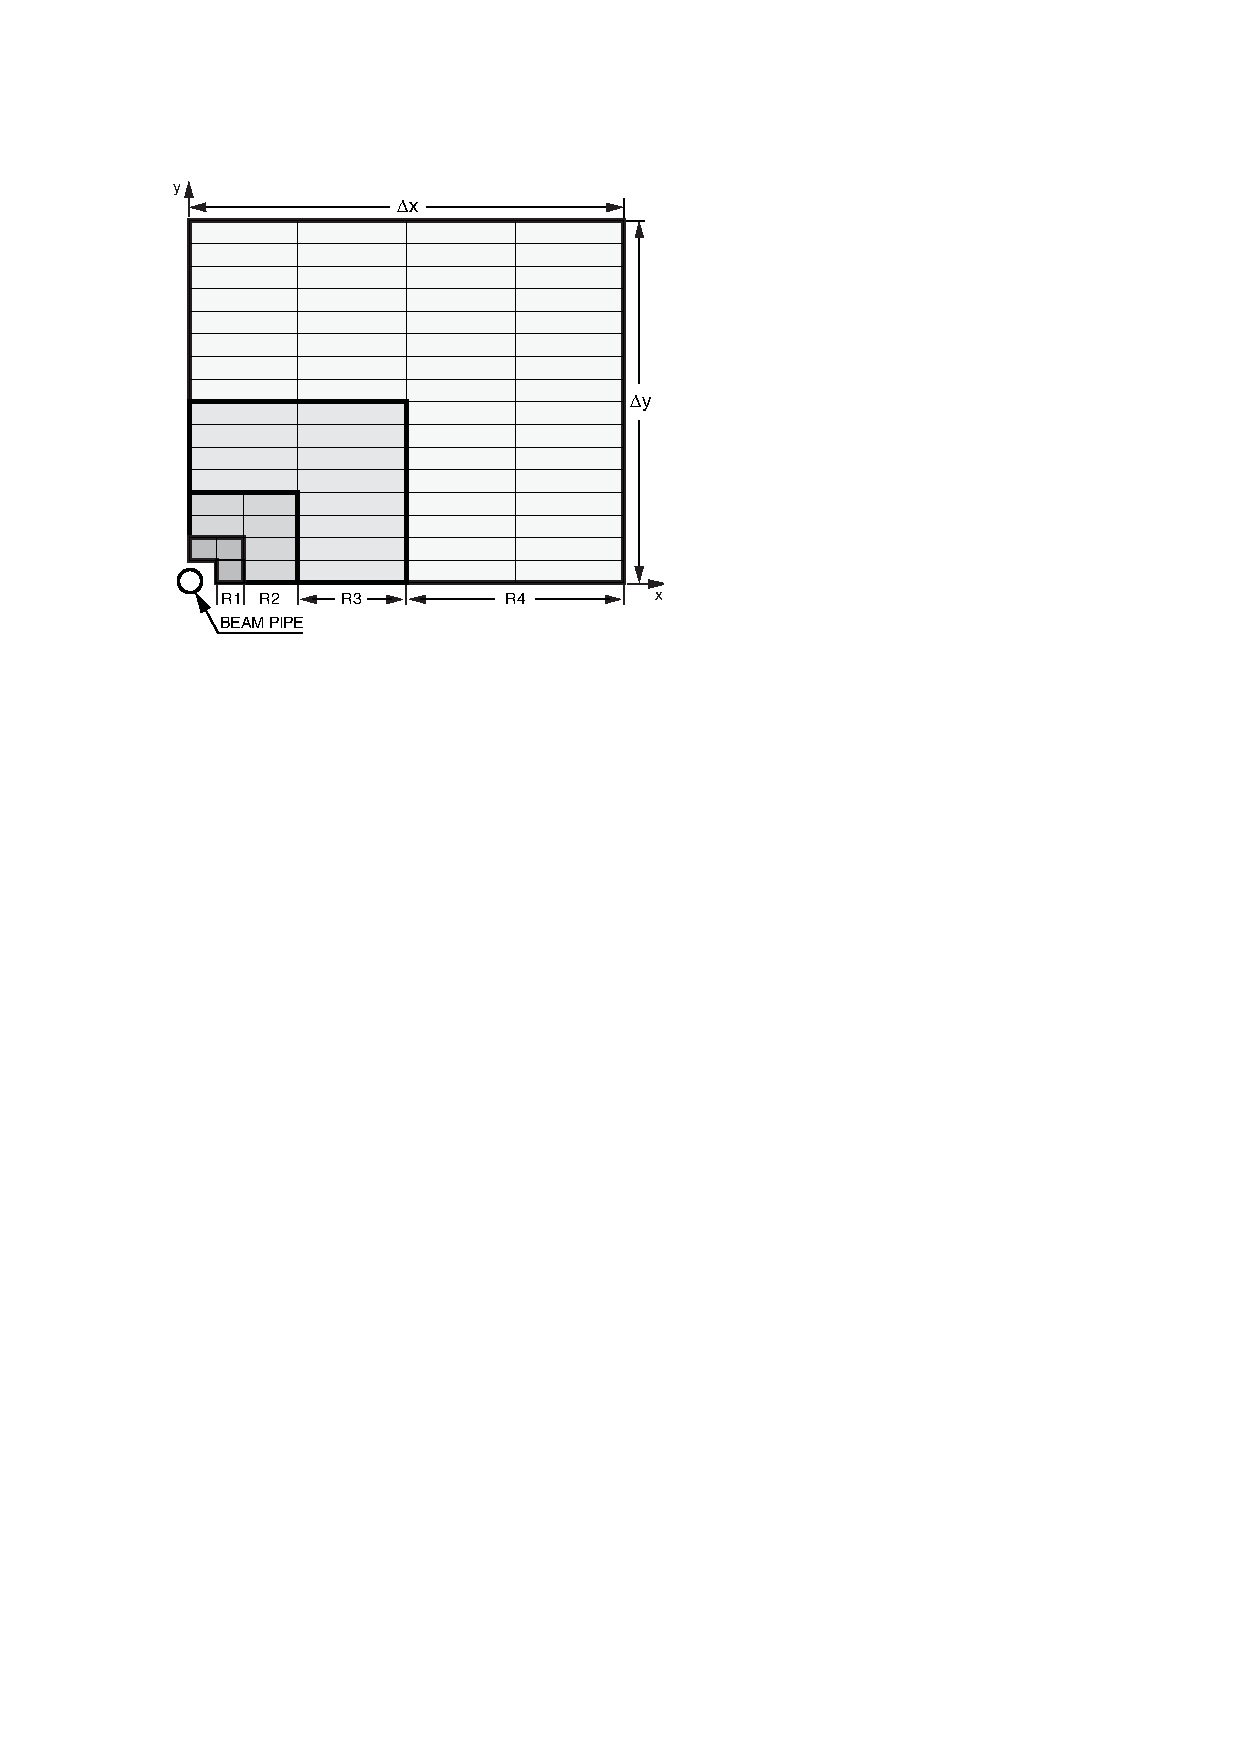
\includegraphics[width=1.0\textwidth]{figs/Detector/muon_cells_layout.pdf}
    \end{subfigure}
    \caption{Side view of the Muon sub-detector (left) and layout of the muon system regions (right), from Ref.~\cite{Alves:2008zz}. For scale, $\Delta x$ and $\Delta y$ vary between 384--594\cm and 320--495\cm in M1--M5 respectively.  }
    \label{fig:Dec_muon_schematic}   
\end{figure}
%%%%%%%%%%%%%%%%%%%%%%%%%%%%%%%%%%%%%%%%%%%%%%%%%%%%%%%%%%

Each of the stations are divided into four regions R1--R4. These are positioned increasingly further from the beam-pipe with increasingly large areas. Each of the regions are segmented into channels; the inner regions have more segmentation than the outer regions such that the particle flux is roughly constant over the four regions.   

The majority of the detector is constructed from Multi Wire Proportional Chambers. These chambers contain a gaseous mixture of carbon dioxide, argon and tetrafluoromethane. When muons pass through this gas they cause ionisation. 
%An array of gold-plated tungsten wires separated by 2\mm are held at a potential difference of around 2.5\,kV with respect to the chamber's conductive walls. The ionised gas and electrons are deflected by the electric field and result in a flow of current. 

Due to the larger flux of particles, the innermost region (R1) of the first station (M1) is instrumented using triple gas electron multiplier detectors. 
%The muons propagating through these detectors ionise a gas mixture made up of argon, carbon dioxide and tetrafluoromethane. The resulting electrons are accelerated toward an anode through three foil layers. The foil layers multiply the number electrons, creating a cascade. 
This type of detector was chosen for the inner region as it is required to be especially radiation hard such that the detector can withstand 10 years of operation.  

\subsection{Trigger}
\label{sec:Dec_trigger}

The primary role of the trigger is to reduce the nominal 40\,MHz beam crossing frequency to a rate that can be recorded. The trigger is composed of two parts: a custom hardware trigger called Level 0 (\lone) that operates at the nominal 40\,MHz beam crossing rate; and an asynchronous High Level Trigger (\hlt) running software algorithms at 1\,MHz. These two stages reduce the event rate to around 2\,kHz, exploiting the characteristics of \bquark- and \cquark-hadron decays to preferentially retain signal decays and discard everything else.

\subsubsection{Level 0}
The \lone trigger takes input from the muon system and calorimeters. These systems feed into a single unit to make a global decision about the event. Although the nominal bunch spacing is 25\ns, the \lone decision is made after 4\mus. During this time the detector signals are stored in a \emph{pipeline} buffer. Half of this 4\mus budget is required for the time-of-flight of the particles and delays in the electronics, leaving the \lone trigger 2\mus to reach a decision about each event.  

The \lone calorimeter trigger uses input from the \spd, \presh, \ecal and \hcal to trigger events. The particles are reconstructed using $2\times2$ cell clusters to calculate the total transverse energy $E_{\text{T}}$ deposited. 
The different particle species are inferred by combining the information from the different calorimeter components.
Hadronic deposits are created by finding the highest energy \hcal cluster with a corresponding \ecal cluster in front of it.
Photons are created from the highest \ecal deposits with corresponding \presh hits. Electrons are created from the highest \ecal deposits with corresponding \presh and at least one \spd hit. 
% \begin{description}
% \item \texttt{L0Hadron}: Hadronic deposits are created by finding the highest energy \hcal cluster with a corresponding \ecal cluster in front of it.  
% \item \texttt{L0Photon}: Photons are created from the highest \ecal deposits with corresponding \presh hits. 
% \item \texttt{L0Electron}: Electrons are created from the highest \ecal deposits with corresponding \presh and at least one \spd hit. 
% \end{description}
If any of these candidates pass corresponding $E_{\text{T}}$ thresholds, then the trigger is initiated. 

The \lone muon trigger selects the two highest \pt muons in each of the four quadrant of the muon system. The event is retained if any of the eight muons' \pt is greater than a threshold, or if any pair has $\pt_{1} \times\ \pt_{2}$ greater than a threshold.

These thresholds are altered when the beam conditions change to maintain a constant \lone output rate. The thresholds used during the 2012 data taking period can be found in Table~\ref{tab:Dec_trigger thresholds}.


\begin{table}[h]
    \centering
      \begin{tabular}{cc}
         \hline
         
         Trigger    & Threshold \\
         \hline
         Muon       & $\pt > 1.76\gevc$\\  
         DiMuon     & $\pt_1\times\pt_2 > 1.6\gevgevcc$\\  
         Hadron     & $\et > 3.7\gev$\\  
         Electron   & $\et > 3.0\gev$\\  
         Photon     & $\et > 3.0\gev$\\  
         \hline
      \end{tabular}
   \caption{Example hardware trigger thresholds used during the 2012 data taking period.}
   \label{tab:Dec_trigger thresholds}
\end{table}

% \begin{description}
% \item \texttt{L0Muon}: Any of the eight muons can fire this trigger if their \pt is greater than a threshold.
% \item \texttt{L0DiMuon}: Pairs of muons can fire this trigger if the quantity $\pt_{1} \times\ \pt_{2}$ is greater than a threshold.
% \end{description}
%The third component of the \lone trigger, the pile-up veto, helps to determine how many primary interactions occurred in a given event. Two \velo $r$-sensors measure the radii of backward tracks, $r_{a}$ and $r_{b}$. For tracks originated at the same vertex the ratio of these is a constant, $k = r_{b}/r_{a}$. The ratio of hits are compared and events with multiple events can be vetoed. 

\subsubsection{High Level Trigger}

The \hlt is a software trigger comprised of \cpp algorithms running on a dedicated processing farm. It is further subdivided into two sections: \hltone and \hlttwo. 
The first stage, \hltone, reduces the rate of events by looking for tracks displaced from the PV.
The software algorithm performs a partial pattern recognition to identify track candidates and to ensure that \Pgamma or \piz \lone candidates are not associated to tracks. This part of the trigger retains around 43\,kHz of \lone-accepted events.
The \velo data is unpacked and a tracking algorithm creates vertices with 5 or more tracks.
Tracks are accepted if they are consistent with originating at one of these vertices. For events selected with the muon \lone lines, the \velo tracks are extrapolated through the dipole field to the muon stations to form muon candidates. 
The \velo or muon candidates are extrapolated through the magnet to the T-stations (\ot and \intr) with a Kalman filter~\cite{Kalmanone,FRUHWIRTH1987444} to account for multiple scattering.




The second stage, \hlttwo, performs a full event reconstruction, allowing explicit decays to be reconstructed. Many different trigger algorithms are included in \hlttwo, reconstructing a wide range of decays. Additionally, a set of inclusive \bquark-hadron decay lines exist, exploiting the common characteristics of these decays. These \emph{topological} trigger lines make decisions based on 2-, 3- or 4-body combinations of tracks that can form a partially or fully reconstructed \bquark-hadron decay~\cite{Williams:2011aza}. These tracks are required to pass a minimum distance of closest approach requirement with respect to each other. The invariant mass of these tracks would span a large range in the case of additional non-reconstructed particles, so a quantity called the corrected mass is calculated instead:
\begin{equation}
m_{\text{corr}} = \sqrt{m^{2} + |\pt'_{\text{miss}}|} + |\pt'_{\text{miss}}|,
\label{eq:hlt_mcorr}
\end{equation}   
where $\pt'_{\text{miss}}$ is the missing momentum transverse to the flight direction of the particle, defined by the vector between the PV and 2-, 3-, or 4-body vertex. Requirements are made to $m_{\text{corr}}$ to ensure the vertex is consistent with a \bquark-hadron decay.
The tracks are required to have a significant impact parameter with respect to the PV. This helps to remove \cquark-hadrons combined with an additional track both originating at the PV. Typical distribution of the corrected mass compared to the measured mass are shown for $\decay{\B}{K\pi\pi}$ decays in Fig.~\ref{fig:Dec_hlt_mcorr}. 

%%%%%%%%%%%%%%%%%%%%%%%%%%%%%%%%%%%%%%%%%%%%%%%%%%%%%%%%%%
\begin{figure}[!h]
    \centering

    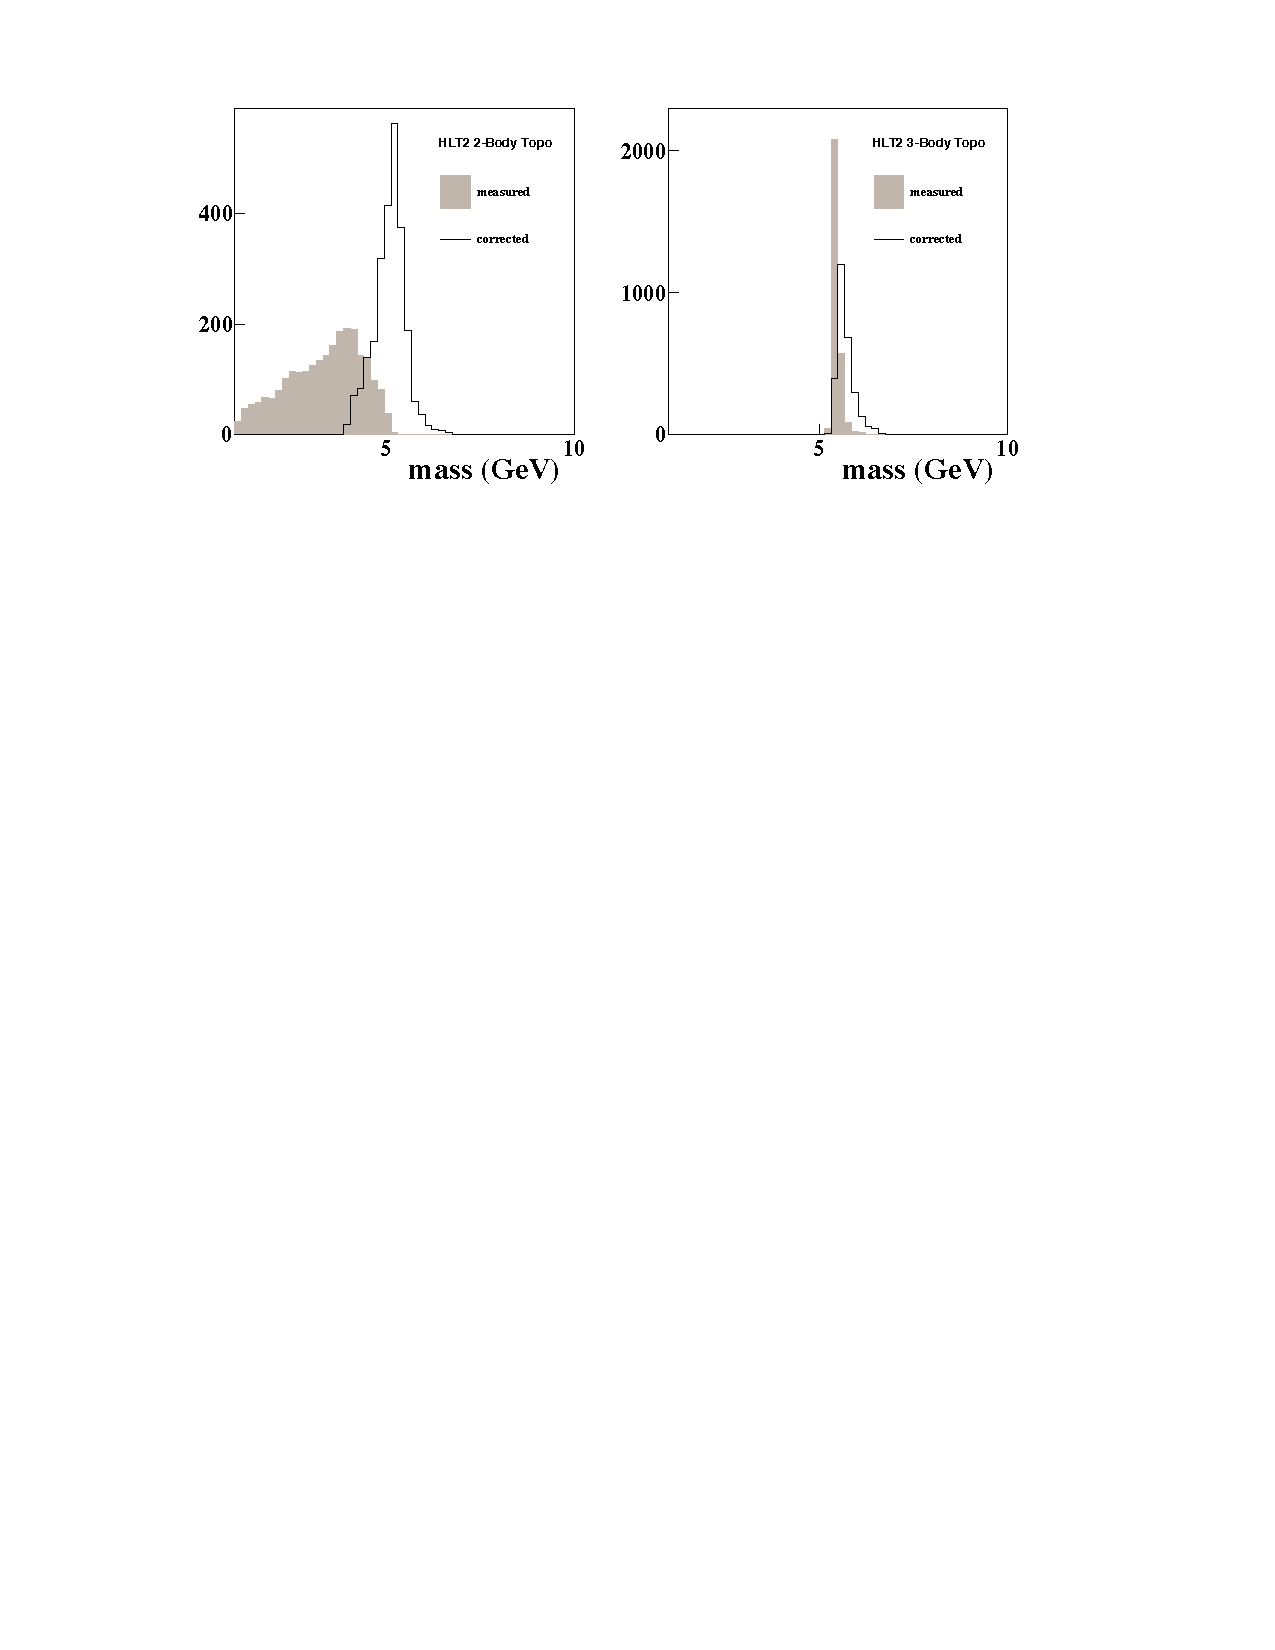
\includegraphics[width=0.6\textwidth]{figs/Detector/InclusiveHlt2Lines.pdf}

    \caption{The invariant mass distributions of $\decay{\B}{K\pi\pi}$ decays using the measured mass (shaded) or corrected mass (line) as defined in Eq.~\ref{eq:hlt_mcorr}, from Ref.~\cite{Williams:2011aza}. This is shown for the 2-body (left) and 3-body (right) inclusive triggers.}
    \label{fig:Dec_hlt_mcorr}   
\end{figure}
%%%%%%%%%%%%%%%%%%%%%%%%%%%%%%%%%%%%%%%%%%%%%%%%%%%%%%%%%%



The \hlt underwent various improvements between Run I and Run II. The number of CPU cores in the Event Filter Farm (EFF) increased from around 29,000 to 52,000. Most notably the \hltone and \hlttwo components were modified to operate asynchronously. This means during Run II the events passing \hltone are stored in a temporary buffer (around 11 petabytes in size) to be processed later by \hlttwo. This allows alignment and calibration to be performed between the running of \hltone and \hlttwo. Dedicated calibration samples are produced by \hltone and processed on the EFF. This includes calculating the \velo and tracking station alignments to optimise the momentum resolution. Additionally, the refractive index of the \rich radiators is calibrated and alignment of the \rich mirror system updated. 
The distribution of the difference between the reconstructed and measured Cherenkov angle in dedicated calibration samples is used to determine a calibration scaling factor. The misalignment is determined by investigating this difference as a function of azimuthal angle.
This allows resolutions of 1.65\mrad and 0.67\mrad to be achieved online for \richone and \richtwo respectively. 
%Dedicated calibration samples are used to determine the difference in the measured and expected Cherenkov angle. A scaling factor  

These improvements in calibration allow the \hlttwo reconstruction to be effectively the same as can be achieved offline. An additional trigger system called the Turbo Stream~\cite{1742-6596-664-8-082004} was added in Run II to create candidates ready for analysis straight out of \hlttwo. However, candidates analysed in this thesis were processed offline.


\subsection{Reconstruction}
%Particles are reconstructed using information from the various sub-detectors. 
The reconstruction of charged and neutral particles is described in this section. 

\subsubsection{Charged particle reconstruction}
Charged particles are reconstructed using tracks passing through the various tracking stations within the \lhcb detector. The curvature of the track as is traverses through the magnetic field allows a precise determination of the momentum. The kinematics of charged particles also require a measurement of the particles energy. However, as the energy is not measured as precisely as the momentum, particles are assigned mass hypotheses, $m$, to determine the energy
\begin{equation}
E = \sqrt{\boldsymbol{p}^{2}+m^{2}}.
\end{equation} 
The invariant mass of n-body combination can therefore be calculated as
\begin{equation}
m^{2}_\text{tot} = E_{\text{tot}}^{2} - \boldsymbol{p}_\text{tot}^2 = \left(\sum^{n}_{i} \sqrt{\boldsymbol{p}_{i}^{2}+m_{i}^{2}}\right)^{2} - \left(\sum^{n}_{i} \boldsymbol{p}_{i}\right)^2
\end{equation}
using the mass hypotheses for each of the contributing tracks.

Charged tracks are reconstructed using the hits in the \velo, \ttracker, \intr and \ot. These are classified into different categories depending on their route taken through the detector as shown in Fig.~\ref{fig:Dec_reco_tracks}. The \intr and \ot are collectively referred to as the T-stations. 

%%%%%%%%%%%%%%%%%%%%%%%%%%%%%%%%%%%%%%%%%%%%%%%%%%%%%%%%%%
\begin{figure}[!h]
    \centering
    \begin{subfigure}[m]{0.4\textwidth}
        \centering
        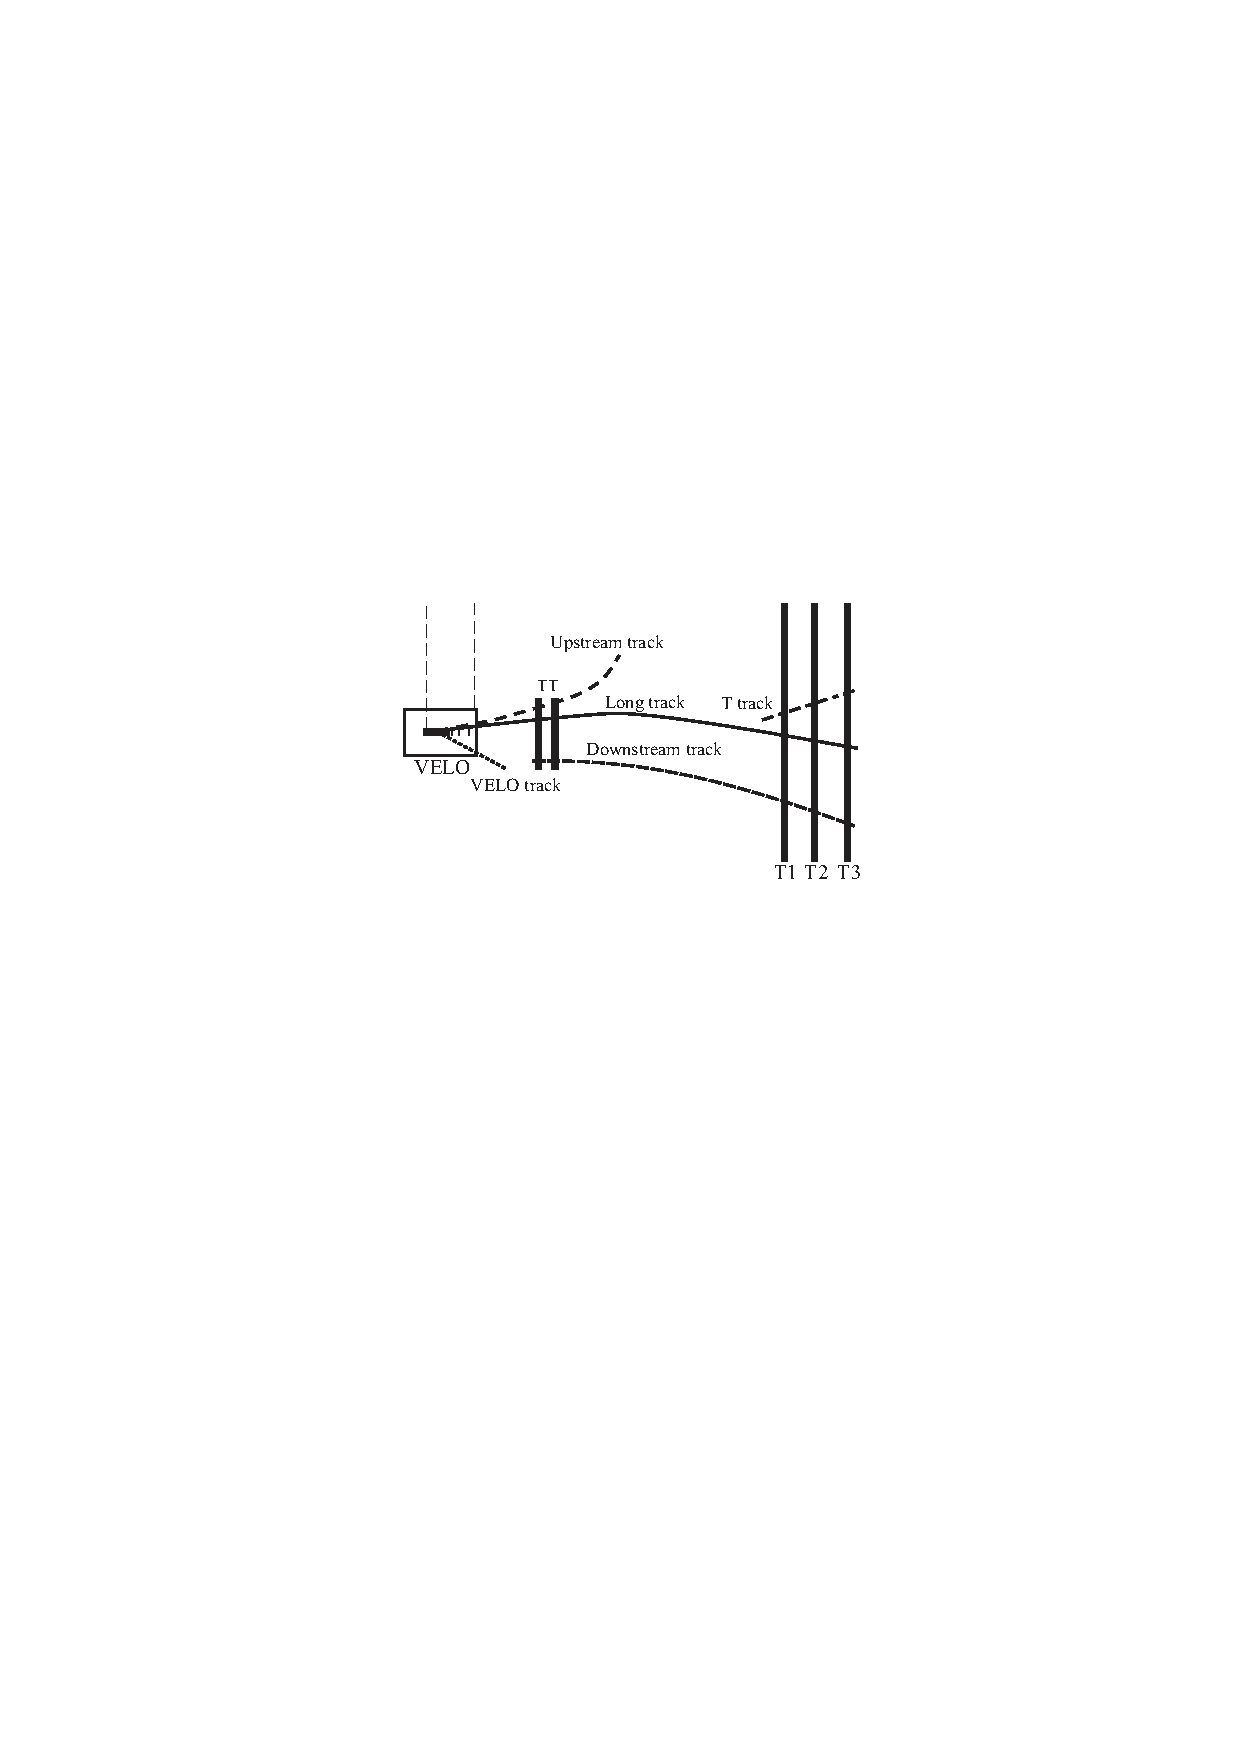
\includegraphics[width=1.0\textwidth]{figs/Detector/reco_track_types.pdf}
    \end{subfigure}
    \begin{subfigure}[m]{0.4\textwidth}
        \centering
        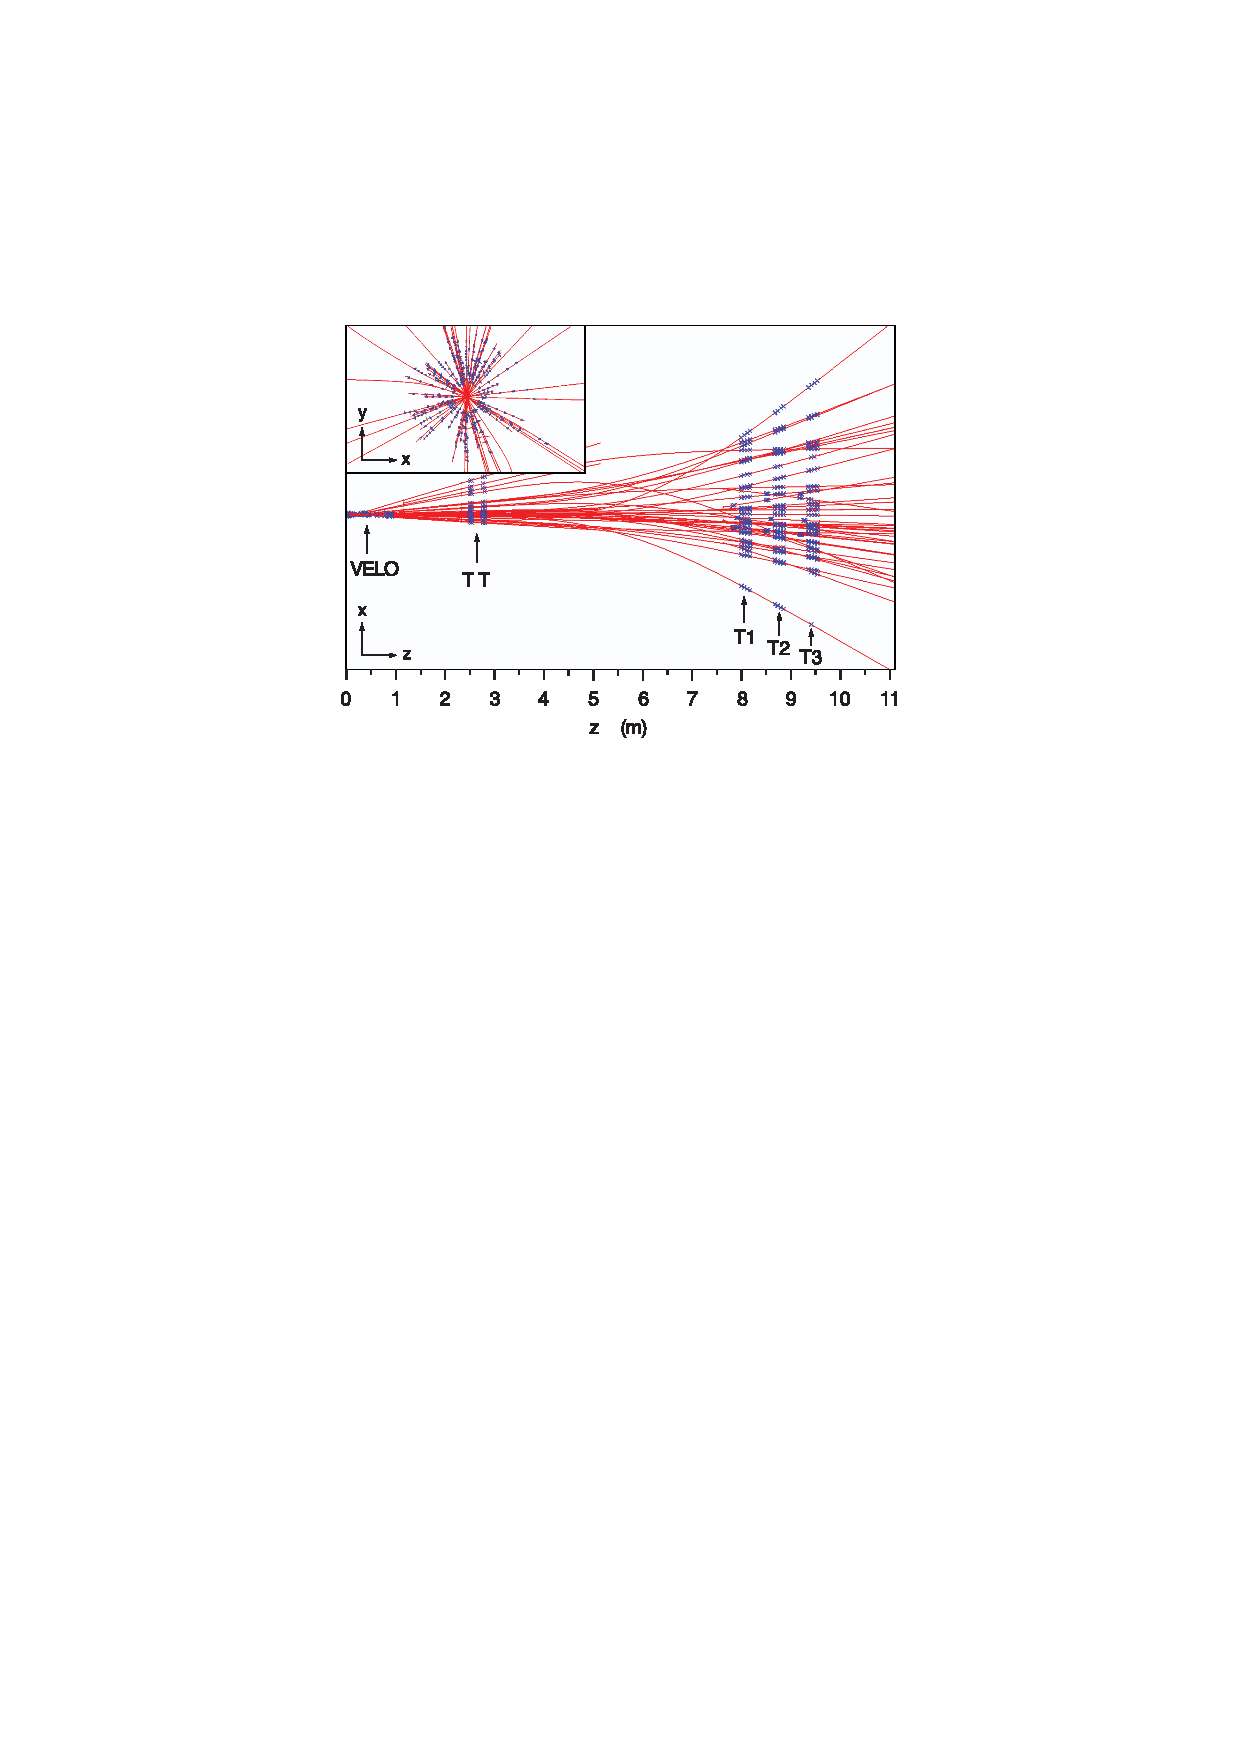
\includegraphics[width=1.0\textwidth]{figs/Detector/reco_track_reco.pdf}
    \end{subfigure}
    \caption{Diagram of the different track reconstruction types (left) and an illustration of the reconstructed tracks in a typical event (right), from Ref.~\cite{LHCb-DP-2014-002}.}
    \label{fig:Dec_reco_tracks}   
\end{figure}
%%%%%%%%%%%%%%%%%%%%%%%%%%%%%%%%%%%%%%%%%%%%%%%%%%%%%%%%%%


\begin{description}
\item \textbf{Long tracks:} these tracks have passed through the \velo, \ttracker and T-stations. This type have the most precise kinematic and topological determination.
\item \textbf{Upstream tracks:} these only pass through the \velo and \ttracker tracker, not the T-stations. This may be because their momentum is too low so the tracks get bent out of the acceptance in the magnetic field.
\item \textbf{Downstream tracks:} these tracks only contain \ttracker and T-station hits. They provide vital information about long-lived particles that decay after they have traversed the \velo.  Two-thirds of \KS mesons come from downstream tracks. 
\item \textbf{VELO tracks:} these tracks only contain hits in the \velo typically because $\theta > 300\mrad$. They can help improve the primary vertex determination. 
\item \textbf{T tracks:} these tracks don't pass through the \velo or \ttracker and are likely to be produced in secondary interaction between the particles and detector material. These tracks are of limited use.
\end{description}

\subsubsection{Charged particle identification}

The identification of charged tracks uses input from the \rich sub-detectors, alongside input from the calorimeter and muon systems to identify electrons and muons respectively. 
As already described in Sec.~\ref{sec:Dec_RICH}, the \rich particle identification is performed by comparing the global event likelihood when changing the particle hypothesis. 
This is combined with information from the calorimeter and muon systems to create an overall particle identification variable
\begin{multline}
\Delta \log{\mathcal{L}_\text{comb}}(X-\pi) =  \Delta \log{\mathcal{L}_\text{RICH}}(X-\pi) + \\
 \Delta \log{\mathcal{L}_\text{Calo}}(X-\pi) + \Delta \log{\mathcal{L}_\text{Muon}}(X-\pi),
\end{multline}
where RICH, Calo and Muon refer to the difference in the log-likelihood of the $X$ and $\pi$ hypothesis as determined by the \rich, calorimeter or muon systems respectively. 

The calorimeter log-likelihood is constructed by comparing the electron to hadron hypotheses. This uses input from the \ecal, \hcal and \presh sub-systems.
% \begin{multline}
% \Delta \log{\mathcal{L}_\text{Calo}}(e - h) =  \Delta \log{\mathcal{L}_\text{\ecal}}(e - h) + \\
%  \Delta \log{\mathcal{L}_\text{\hcal}}(e - h) + \Delta \log{\mathcal{L}_\text{\presh}}(e - h)
% \end{multline}
For the \hcal and \presh this input is determined using the energy deposited. For the \ecal this is constructed comparing the ratio of energy to momentum, $E/pc$, for the candidates, which peaks around one for electrons and at lower values for hadrons. Additionally, the centre of the \ecal deposit and extrapolated track position are compared.     

The muon system log-likelihood is determined by extrapolating the track in question to the muon stations. The average squared distance of the extrapolated positions and hits in the stations are used to compare the muon to non-muon hypothesis.   

\subsubsection{Neutral particle reconstruction}

The energy of neutral particles are determined directly from the calorimeter system. This system is calibrated during running to maintain the optimal resolution.  

\begin{description}
\item\textbf{Photons:} Isolated \ecal clusters with an corresponding cluster in the \presh are used to create photon candidates. The energy is determined from the total energy deposited in the \ecal and \presh. 
\item \textbf{Neutral pions:} These mesons decay dominantly to two photons, however the reconstruction depends on the transverse momentum of the \piz. For low \pt decays the two photons are well separated (\emph{resolved}) leading to two photon deposits. For higher \pt decays the two photon deposits overlap leading to a single \ecal cluster (\emph{merged}). Merged \piz are rarely used in analysis.
\item \textbf{Bremsstrahlung correction:} as a result of their small mass, electrons can radiate Bremsstrahlung photons. If this occurred before the magnetic field the photon produced results in a separate \ecal cluster. If this radiation occurs after the magnet the photon cluster can overlaps with the electron cluster. Clusters in the \ecal that are consistent with radiated Bremsstrahlung photons are used to correct the measured energy of the electron.
\end{description}



%\section{Luminosity determinations and \velo resolution}
\section{Luminosity determination}
The observed rate, $R$, of a particular physical processes at particle colliders are defined by the luminosity $\mathcal{L}$ and the cross-section of the process, $\sigma$, 
\begin{equation}
R = \mathcal{L}\sigma.
\label{eq:lumi}
\end{equation}
Experimentally, the numbers of particular processes are counted. To obtain cross-section measurements, precise measurements of the luminosity over the data-collection period are required.

The luminosity can be determined \emph{indirectly}, by reversing Eq.~\ref{eq:lumi} and inputting a well-known cross section for a calibration process, or \emph{directly}, by calculating it from the machine parameters,
\begin{equation}
\mathcal{L} = f_{\text{rev}}N_{1}N_{2}\Omega,
\end{equation}
where $f_{\text{rev}}$ is the revolution frequency, $N_{1}$ and $N_{2}$ are the number of protons in the two beams and $\Omega$ is a geometrical factor that quantifies the overlap of two colliding bunches~\cite{1748-0221-9-12-P12005}. 
For two beams of ultra-relativistic particles the overlap integral can be approximated as 
\begin{equation}
\Omega = 2c\int \rho_{1}(x,y,z,t)\rho_{2}(x,y,z,t)\,dx\,dy\,dz\,dt 
\end{equation}
where $\rho$ describes the particle density distribution.
Two methods used to \emph{directly} determine the luminosity at \lhcb are described here.

% \begin{itemize}
% \item Van der Meer scans
% \item Beam gas imaging
% \end{itemize} 


\subsection{Van der Meer scans}

The luminosity of the collisions can be determined using the van der Meer technique~\cite{VanDerMeer}. This involves sweeping two beams across each other in the transverse plane. By measuring the interaction rate as a function of the beam displacement, the overlap of the two beams can be determined, and hence the absolute luminosity. The two beams are moved simultaneously, alternating between the two transverse directions as shown in Fig.~\ref{fig:Dec_vdm_scan}.

%%%%%%%%%%%%%%%%%%%%%%%%%%%%%%%%%%%%%%%%%%%%%%%%%%%%%%%%%%
\begin{figure}[!h]
    \centering
    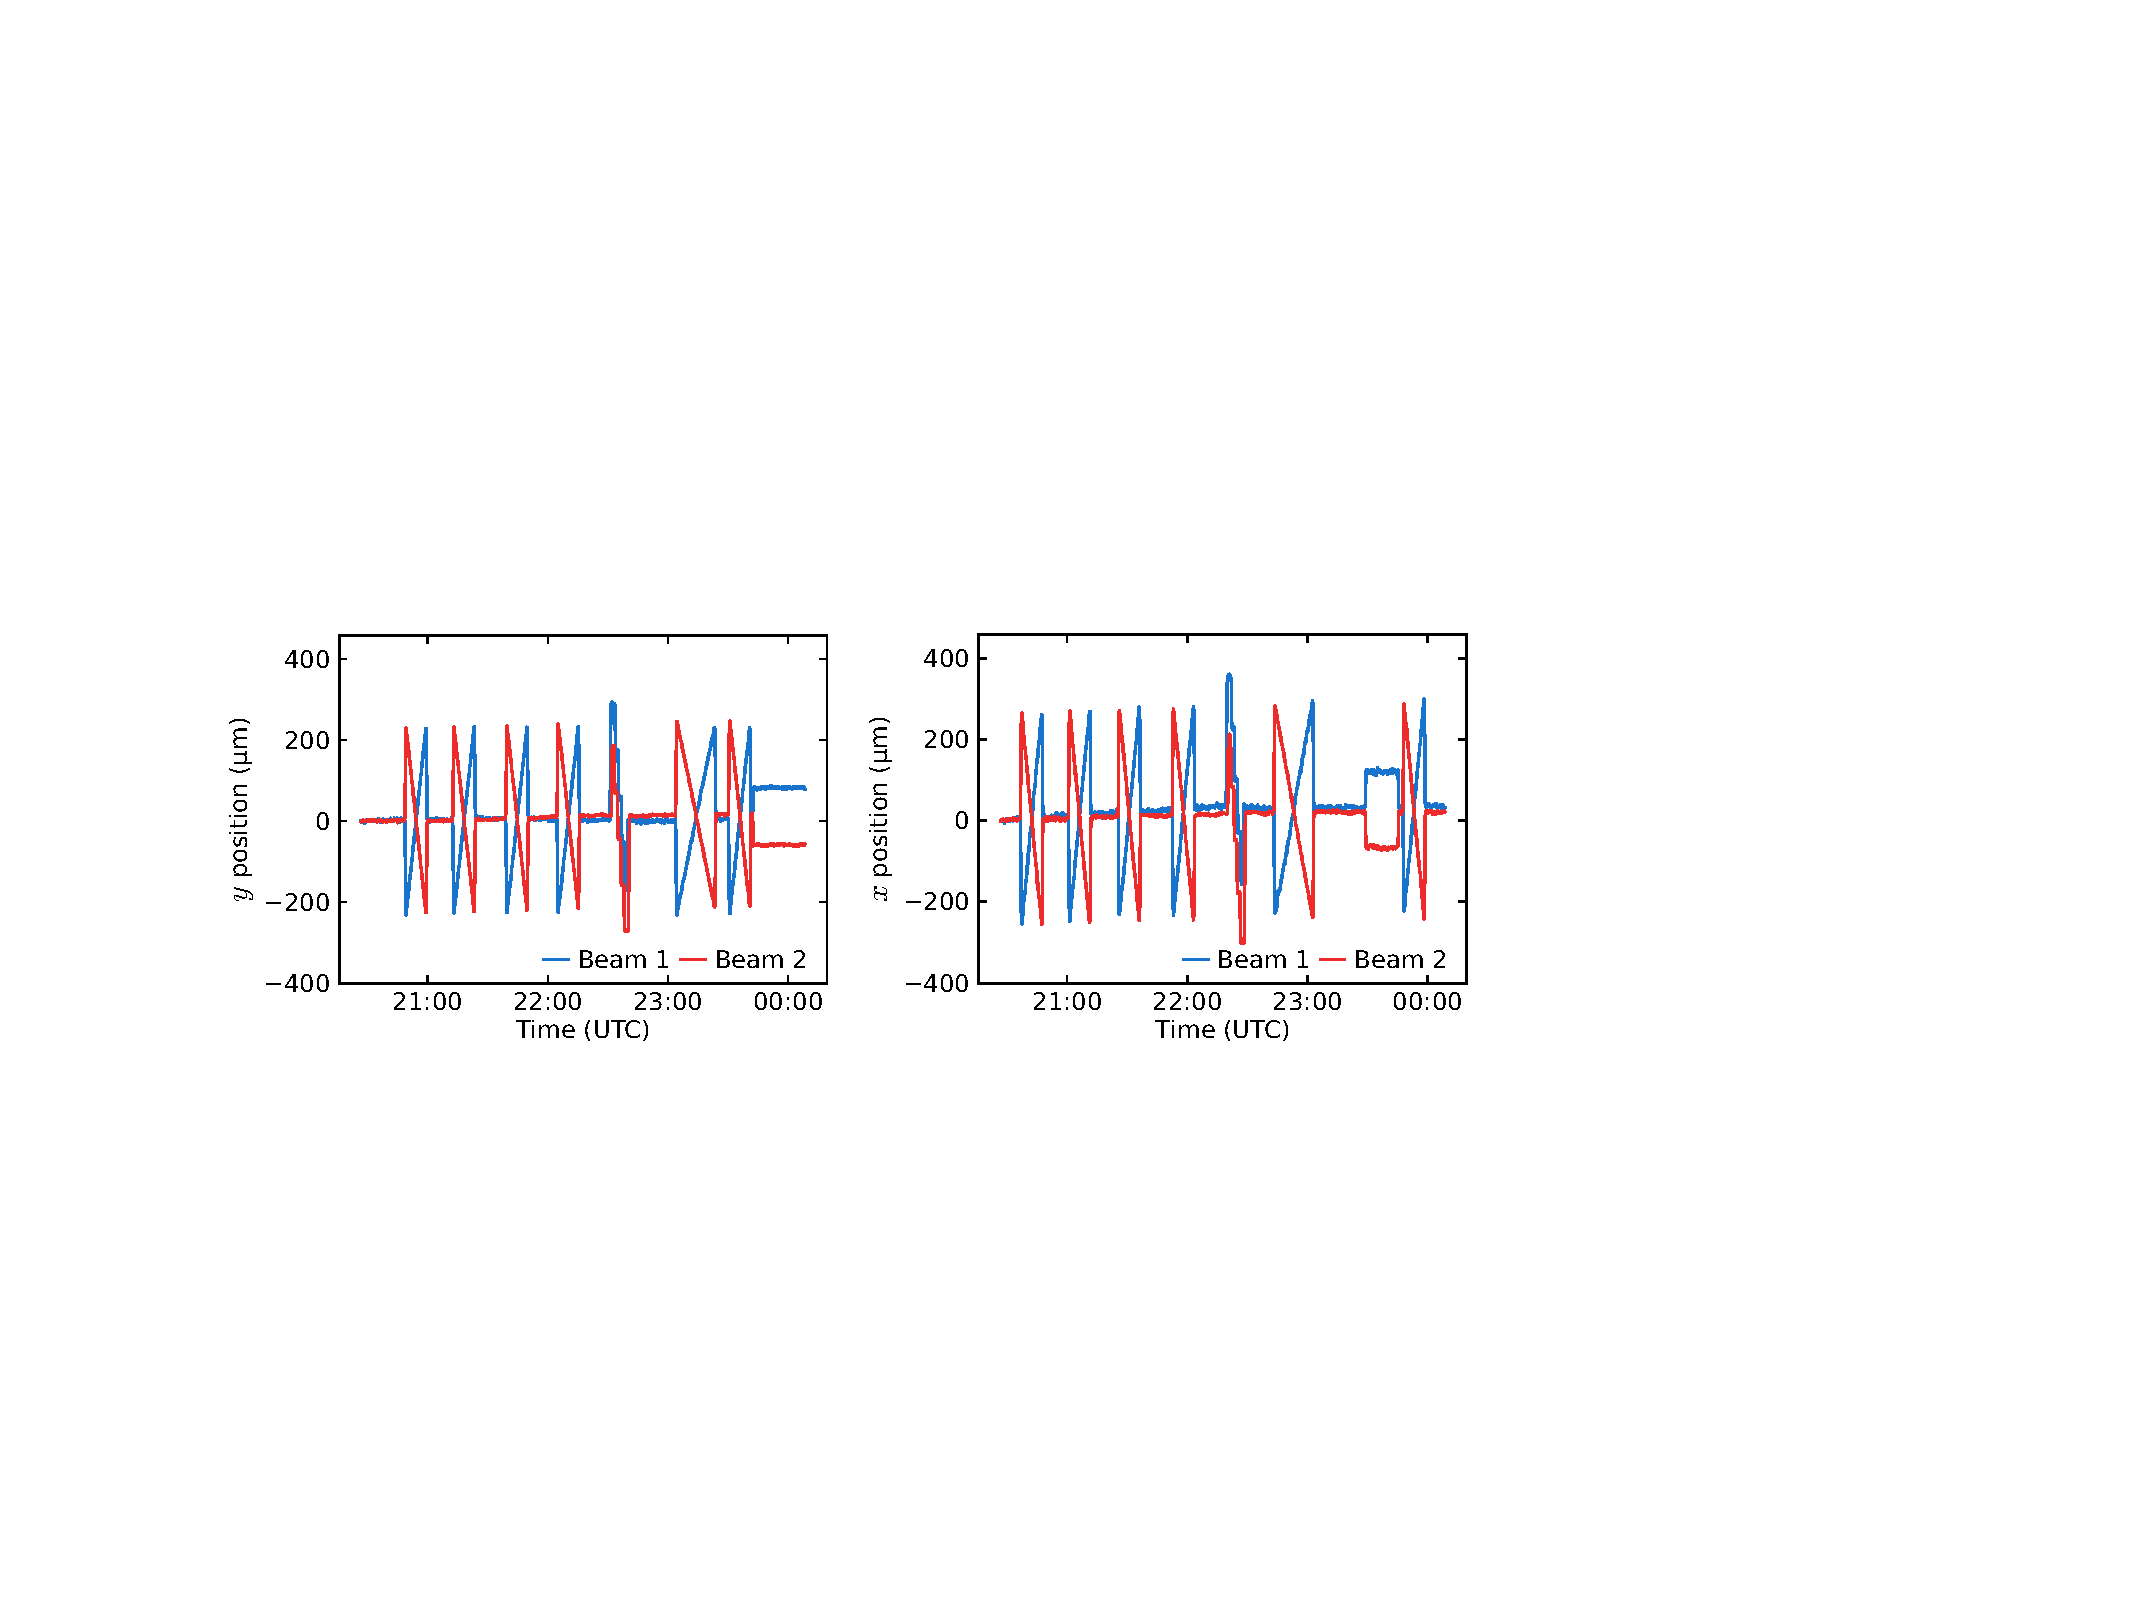
\includegraphics[width=1.0\textwidth]{figs/Detector/lumi_plots.pdf}
    \caption{Beam positions in the $y$-axis (left) and $x$-axis (right) during a van der Meer scan to determine the absolute luminosity, from Ref.~\cite{1748-0221-9-12-P12005}.}
    \label{fig:Dec_vdm_scan}   
\end{figure}
%%%%%%%%%%%%%%%%%%%%%%%%%%%%%%%%%%%%%%%%%%%%%%%%%%%%%%%%%%
The absolute luminosity is calculated for the specific van der Meer scan fills, and extrapolated to the full data set using the interaction rate of standard processes. The effective visible cross-section $\sigma_{\text{vis}}$ is calibrated for the standard processes during the absolute luminosity determination fill. The total integrated luminosity for a data sample can be determined by the accumulated rate of the standard process.  


\subsection{Beam gas imaging}

The luminosity can also be calculated by exploiting the interactions between the beams and residual gas molecules in the beam pipe vacuum. The precision of the \velo allows the beam-gas interaction vertices to be reconstructed. These vertices allow the beam position, shape and angle to be determined. The typical distribution of beam-gas vertices in the $xz$ and $yz$ planes are shown in Fig.~\ref{fig:Dec_bgi_distro}. The crossing angle in the horizontal plane is clearly visible. 
%%%%%%%%%%%%%%%%%%%%%%%%%%%%%%%%%%%%%%%%%%%%%%%%%%%%%%%%%%
\begin{figure}[!h]
    \centering
    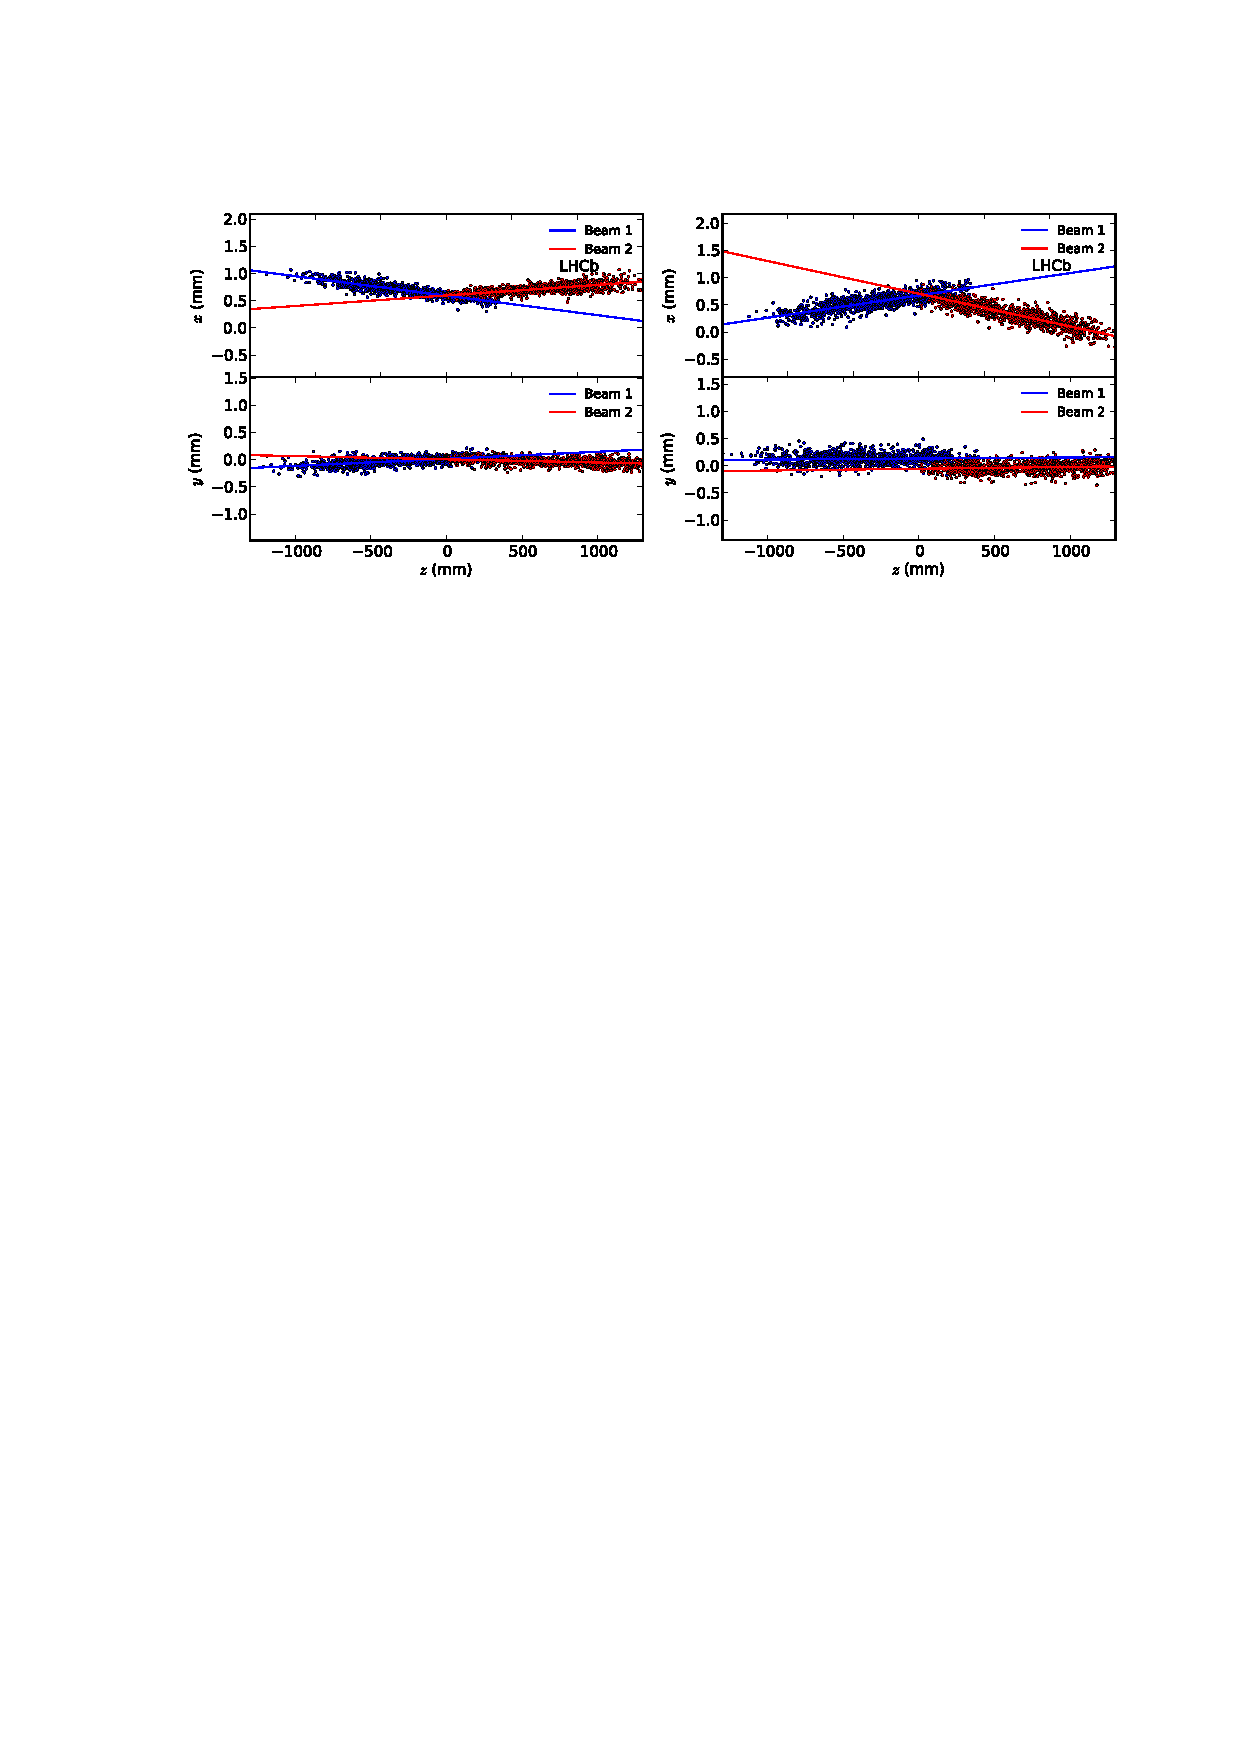
\includegraphics[width=1.0\textwidth]{figs/Detector/lumi_bgi_distro.pdf}
    \caption{The positions of beam-gas interactions reconstructed in the \velo sub-detector, from Ref.~\cite{1748-0221-9-12-P12005}.}
    \label{fig:Dec_bgi_distro}   
\end{figure}
%%%%%%%%%%%%%%%%%%%%%%%%%%%%%%%%%%%%%%%%%%%%%%%%%%%%%%%%%%
The overlap of the two bunches is determined by first fitting the beam profiles to obtain the three dimensional density $\rho(x,y,z)$ for each beam. This is possible due to beam crossings in which only one of the two beams were present. This means all reconstructed beam-gas interactions can be attributed to the single beam. 


\subsubsection{\velo resolution}

The distributions of the beam gas interactions as reconstructed by the \velo sub-detector are not simply the beam profiles, as the vertex position resolution must be accounted for. The resulting distribution is the convolution of the beam profile and resolution distribution. The \velo vertex resolution is strongly dependent on the number of tracks used to create the vertex, as well as the longitudinal position of the vertex. 

The resolution of vertices is estimated by splitting the tracks contributing to vertices into two random sub-samples. The vertex position for each of these sub-samples, $v_{1,2}$ is determined and the difference in the vertex positions $\Delta v = v_{1}-v_{2}$ is found. The width of the $\Delta v$ distribution when splitting many vertices is used as a proxy for the resolution. 
The resolution determined for different values vertex track multiplicity and longitudinal position is shown in Fig.~\ref{fig:Dec_bgi_res}.
%%%%%%%%%%%%%%%%%%%%%%%%%%%%%%%%%%%%%%%%%%%%%%%%%%%%%%%%%%
\begin{figure}[!h]
    \centering
    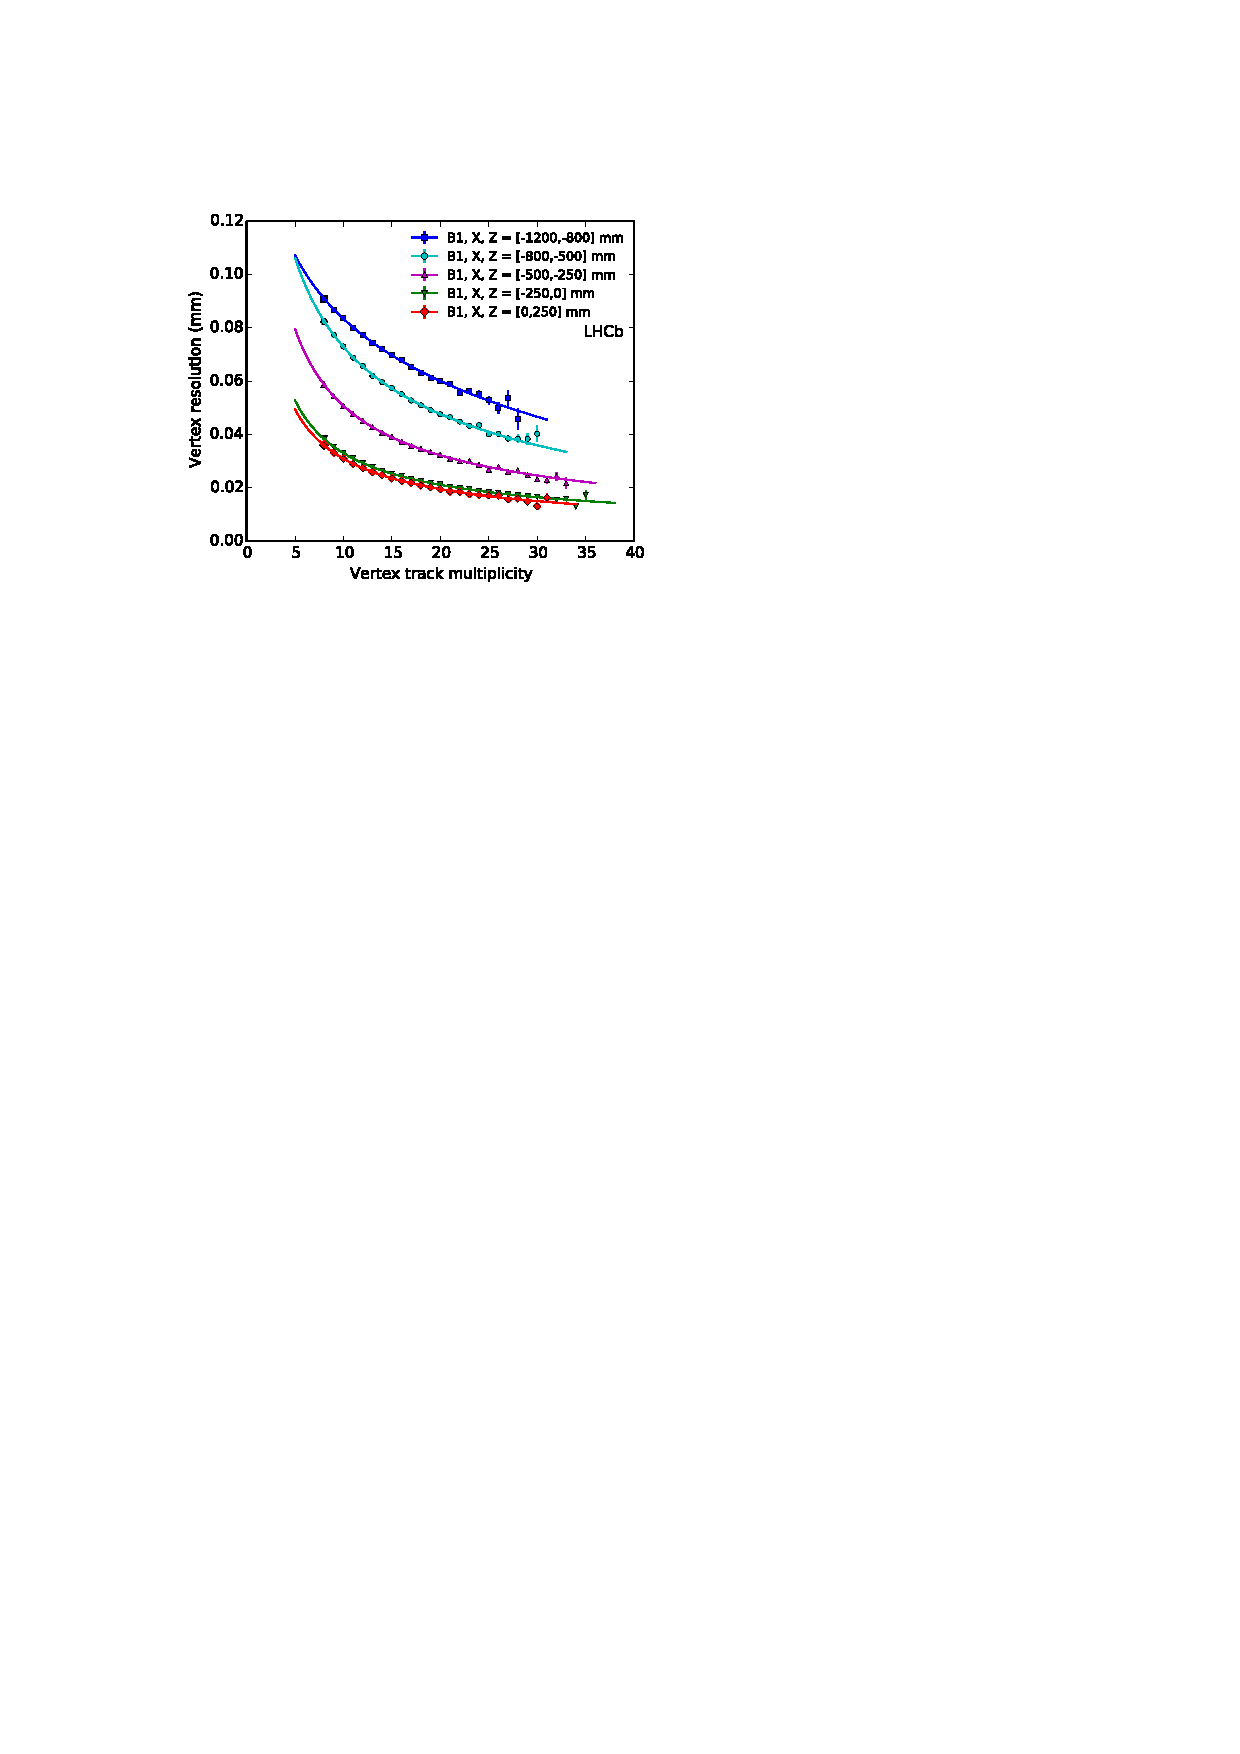
\includegraphics[width=1.0\textwidth]{figs/Detector/lumi_bgi_track_z_res.pdf}
    \caption{The resolution of beam-gas interactions as a function of the vertex track multiplicity and longitudinal position, for Beam 1 (B1) and Beam 2 (B2), from Ref.~\cite{1748-0221-9-12-P12005}.}
    \label{fig:Dec_bgi_res}   
\end{figure}
%%%%%%%%%%%%%%%%%%%%%%%%%%%%%%%%%%%%%%%%%%%%%%%%%%%%%%%%%%
These resolution values are used to subtract the smearing from the \velo resolution such that the beam profiles can be accurately determined. 


\subsubsection{Real-time beam measurements}
\label{sec:Dec_real_time}
The beam gas imaging method additionally allows measurements of the beam profiles to be made in real-time during data taking. 
As detailed in Sec.~\ref{sec:Dec_beam_conds} the \lhc runs with a smaller number of bunches than the full capacity would allow. The distribution of filled and empty bunch slots are usually chosen to maximise the luminosity for \atlas and \cms, therefore only a subset of the total bunches collide at \lhcb. Those beam crossings in which only one of the two bunches pass through \lhcb can be used to make measurements of the beam-gas interactions during normal running.
These provide information about the beam angle, positions and shapes. The shape parameters can be used to calculate the emittance of the beams. This information is published back to the \lhc, providing important information about the performance of the machine.

A fraction of collisions are sent to a dedicated monitoring farm to be analysed in real-time. Measurements are made of the beam positions and widths averaged over all bunches in each beam. 
%Examples of the measurements of Beam 1 and Beam 2 in the $x$-dimension are shown in Fig.~\ref{fig:Dec_bgi_realtime}. 
Plots can be monitored during data taking in the \lhcb control room and the values are transmitted to the \lhc. During normal data taking updates are published approximately every five minutes, depending on the \lhc filling-scheme. 
%Additionally, measurement of individual bunches are produced, but at a much lower frequency due to the limited statistics. 

% %%%%%%%%%%%%%%%%%%%%%%%%%%%%%%%%%%%%%%%%%%%%%%%%%%%%%%%%%%
% \begin{figure}[!h]
%     \centering
%     \begin{subfigure}[m]{0.7\textwidth}
%         \centering
%         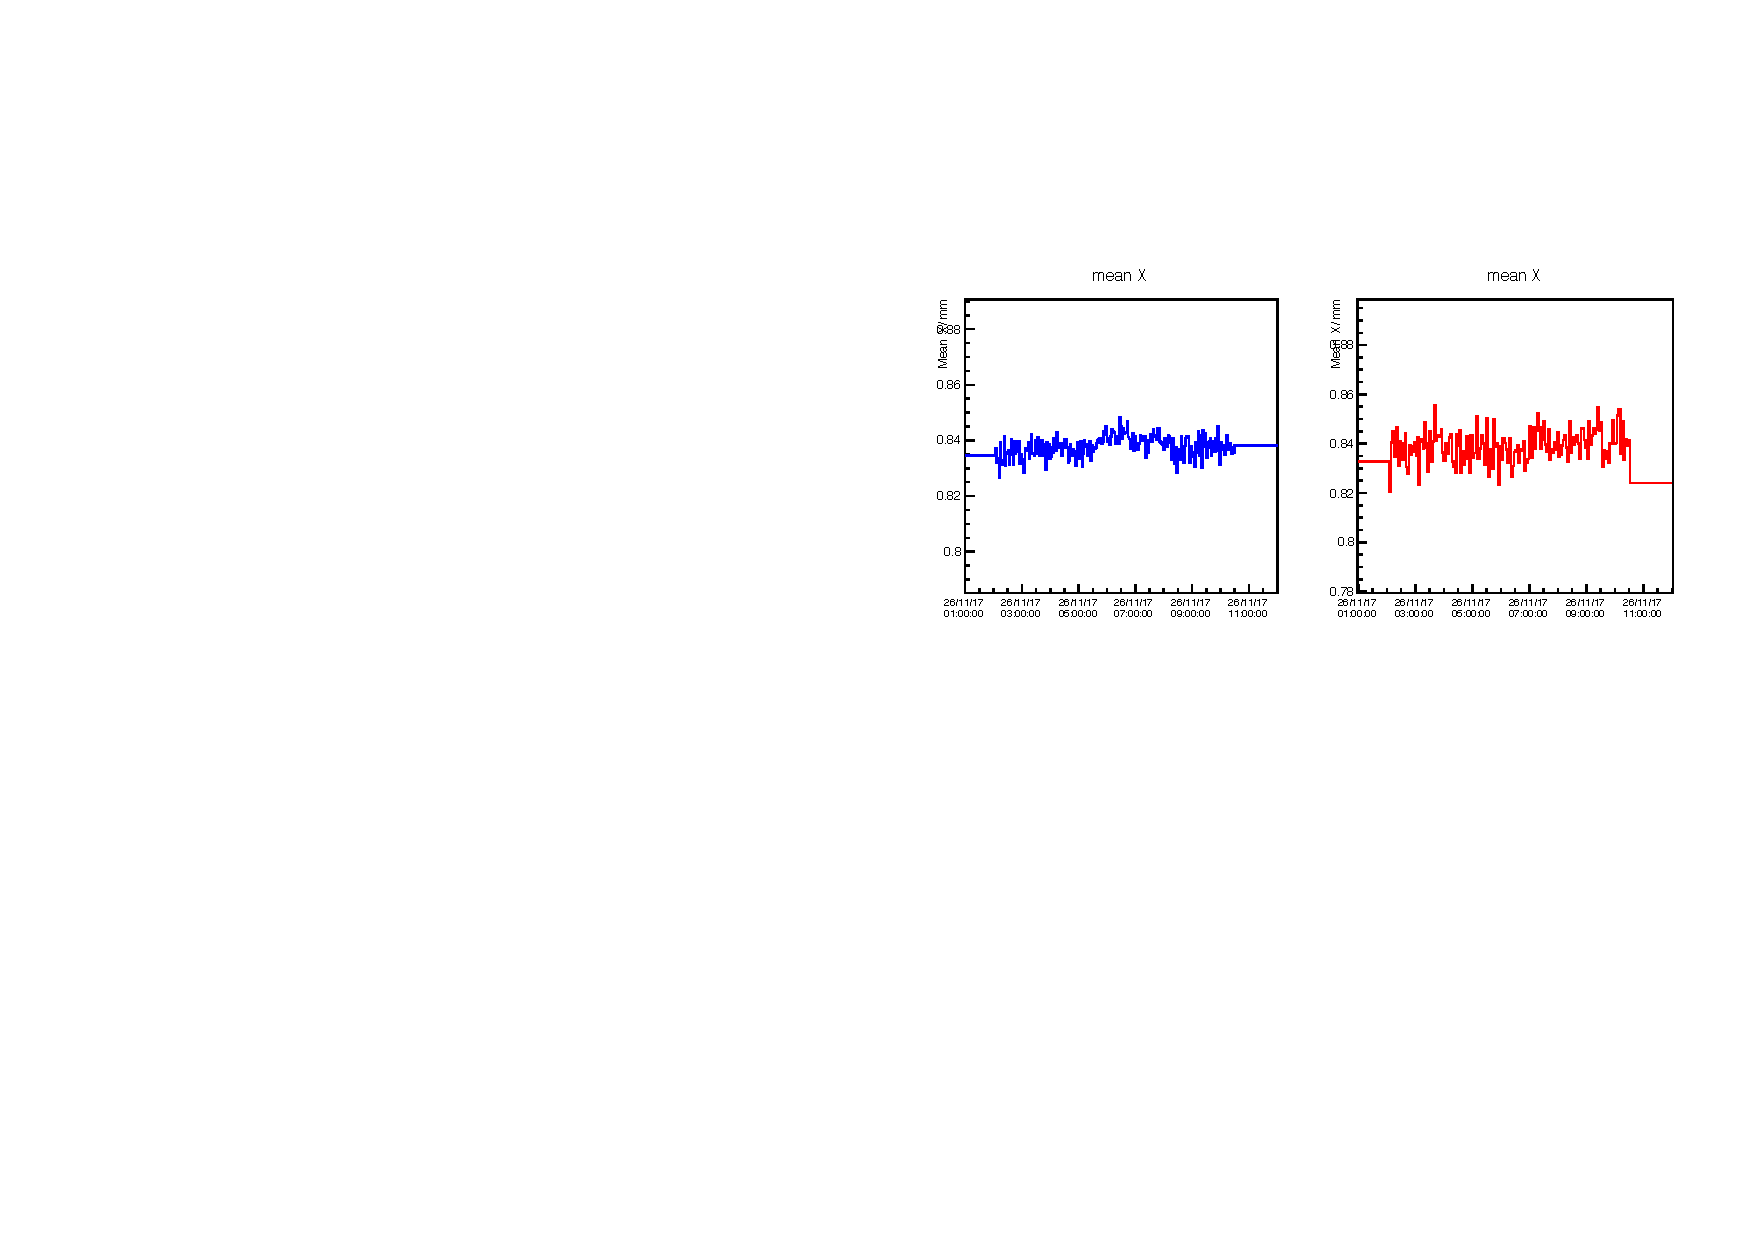
\includegraphics[width=1.0\textwidth]{figs/Detector/Beam_position_realtime.pdf}
%     \end{subfigure}
%     \begin{subfigure}[m]{0.7\textwidth}
%         \centering
%         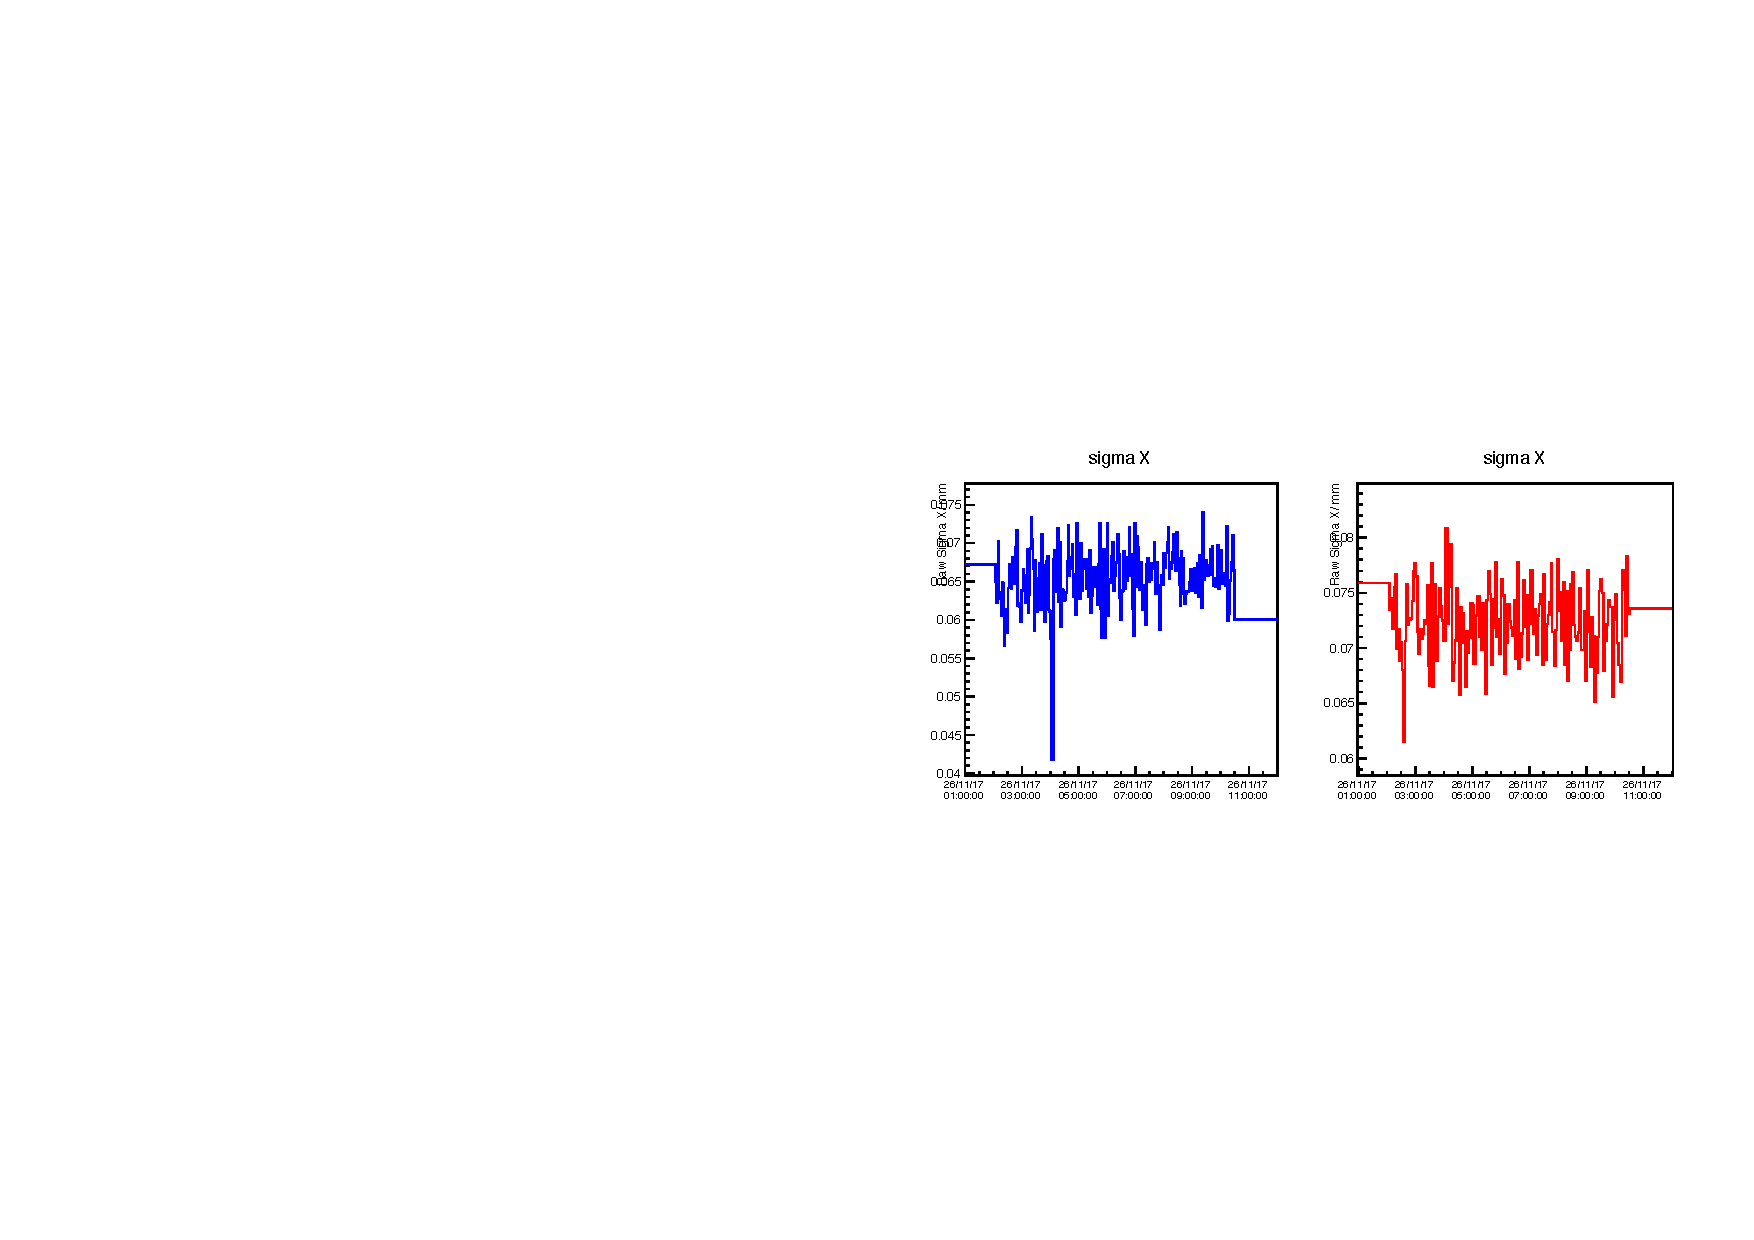
\includegraphics[width=1.0\textwidth]{figs/Detector/Beam_sigma_realtime.pdf}
%     \end{subfigure}
%     \caption{The mean position (top) and width (bottom) of Beam 1 (left) and Beam 2 (right) bunches in the $x$-dimension. These values were collected in real time during one fill and appear as presented in the \lhcb control room.}
%     \label{fig:Dec_bgi_realtime}   
% \end{figure}
% %%%%%%%%%%%%%%%%%%%%%%%%%%%%%%%%%%%%%%%%%%%%%%%%%%%%%%%%%%

%The beam-gas collisions can be re-analysed offline to exploit the full available statistics. 
A dedicated \lhc-wide cross-calibration of emittance measuring devices was performed in 2016~\cite{Hadavizadeh:IPAC2017-MOPAB131}. The increased statistics available offline allow the positions and widths of individual bunches to be determined throughout the fill as shown in Fig.~\ref{fig:Dec_bgi_fill}. During this calibration fill gas was injected into the beam-pipe vacuum within the \velo to increase the rate of beam-gas interactions. The \lhcb beam-gas imaging measurements were found to be mostly consistent with the other beam-size measurement devices around the \lhc, however the specific optics of the \lhc beams resulted in large uncertainties.   
%%%%%%%%%%%%%%%%%%%%%%%%%%%%%%%%%%%%%%%%%%%%%%%%%%%%%%%%%%
\begin{figure}[!h]
    \centering
    \begin{subfigure}[m]{0.49\textwidth}
        \centering
        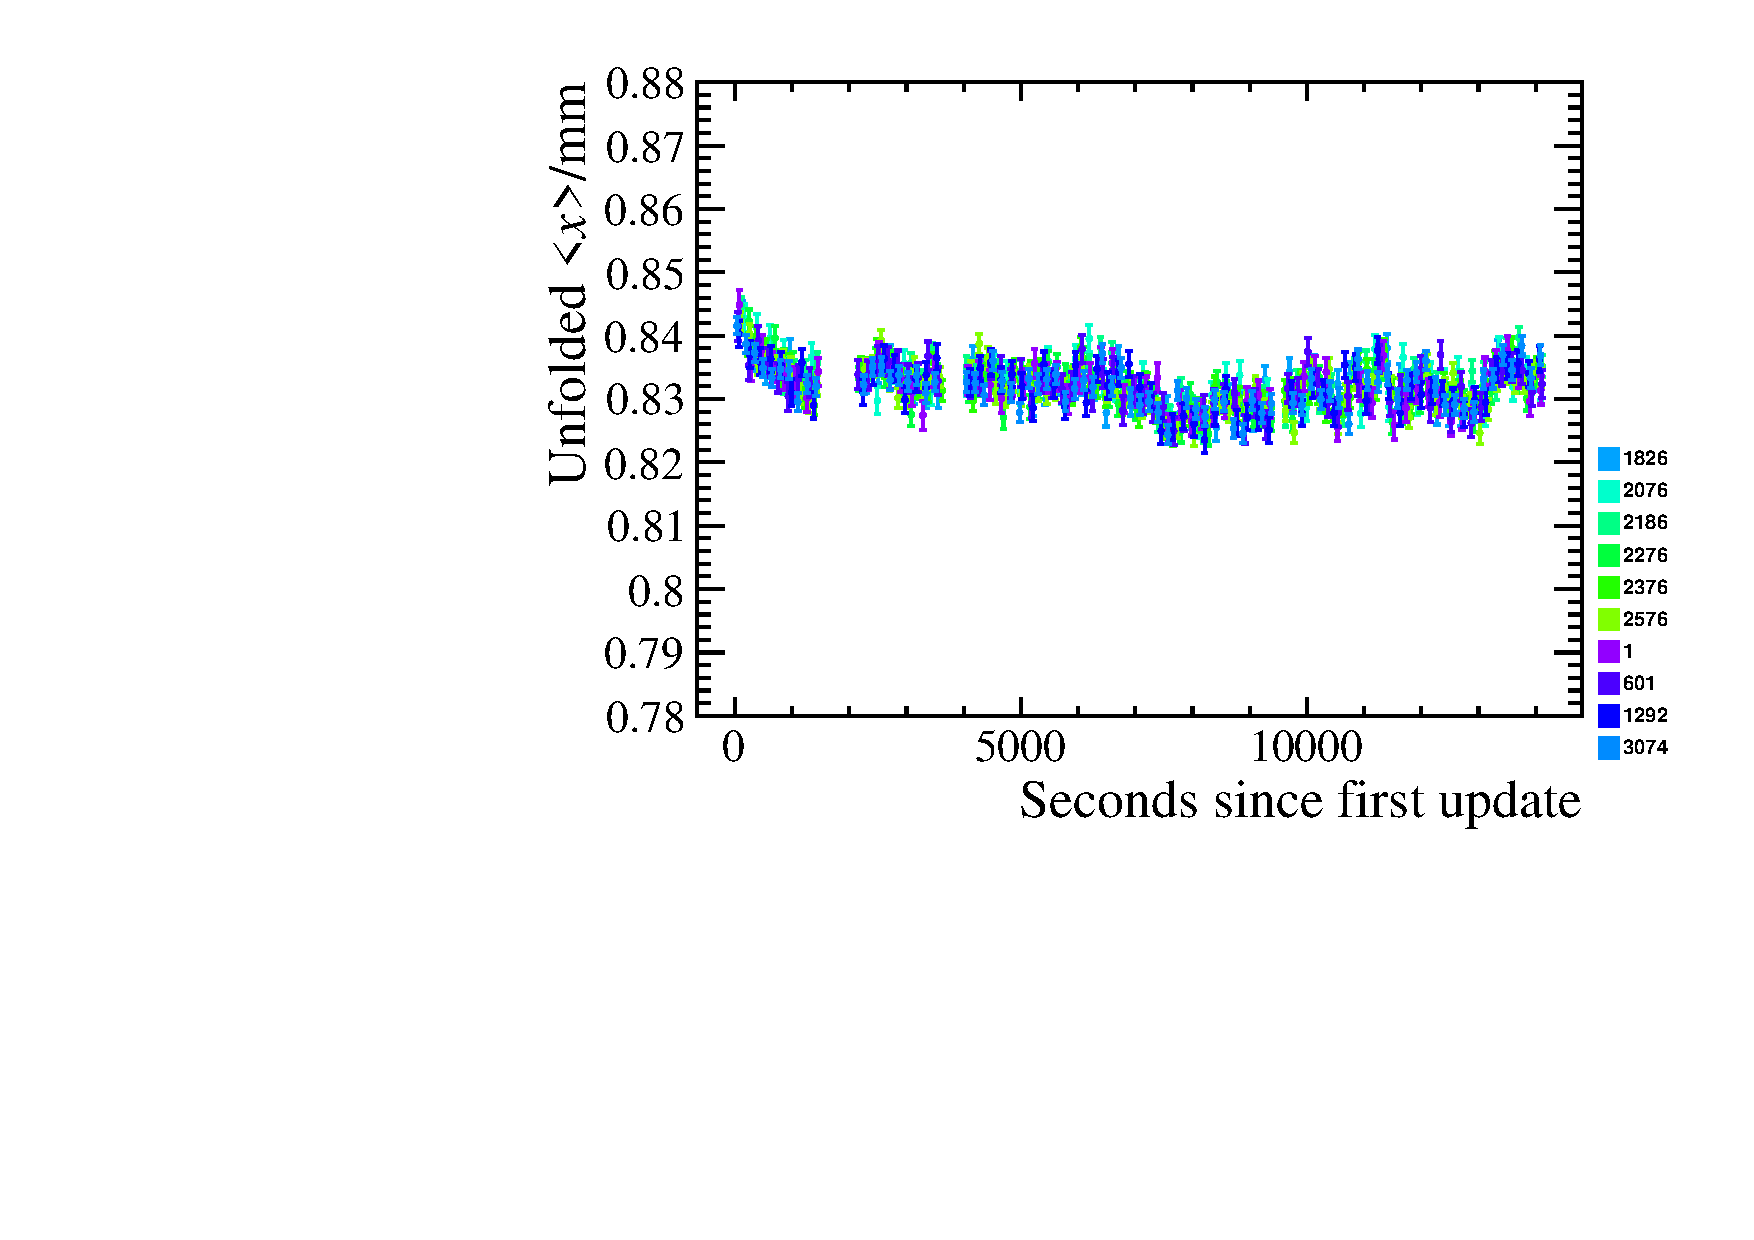
\includegraphics[width=1.0\textwidth]{figs/Detector/PerBXID_MeanX_unfolded_Beam1.pdf}
    \end{subfigure}
    \begin{subfigure}[m]{0.49\textwidth}
        \centering
        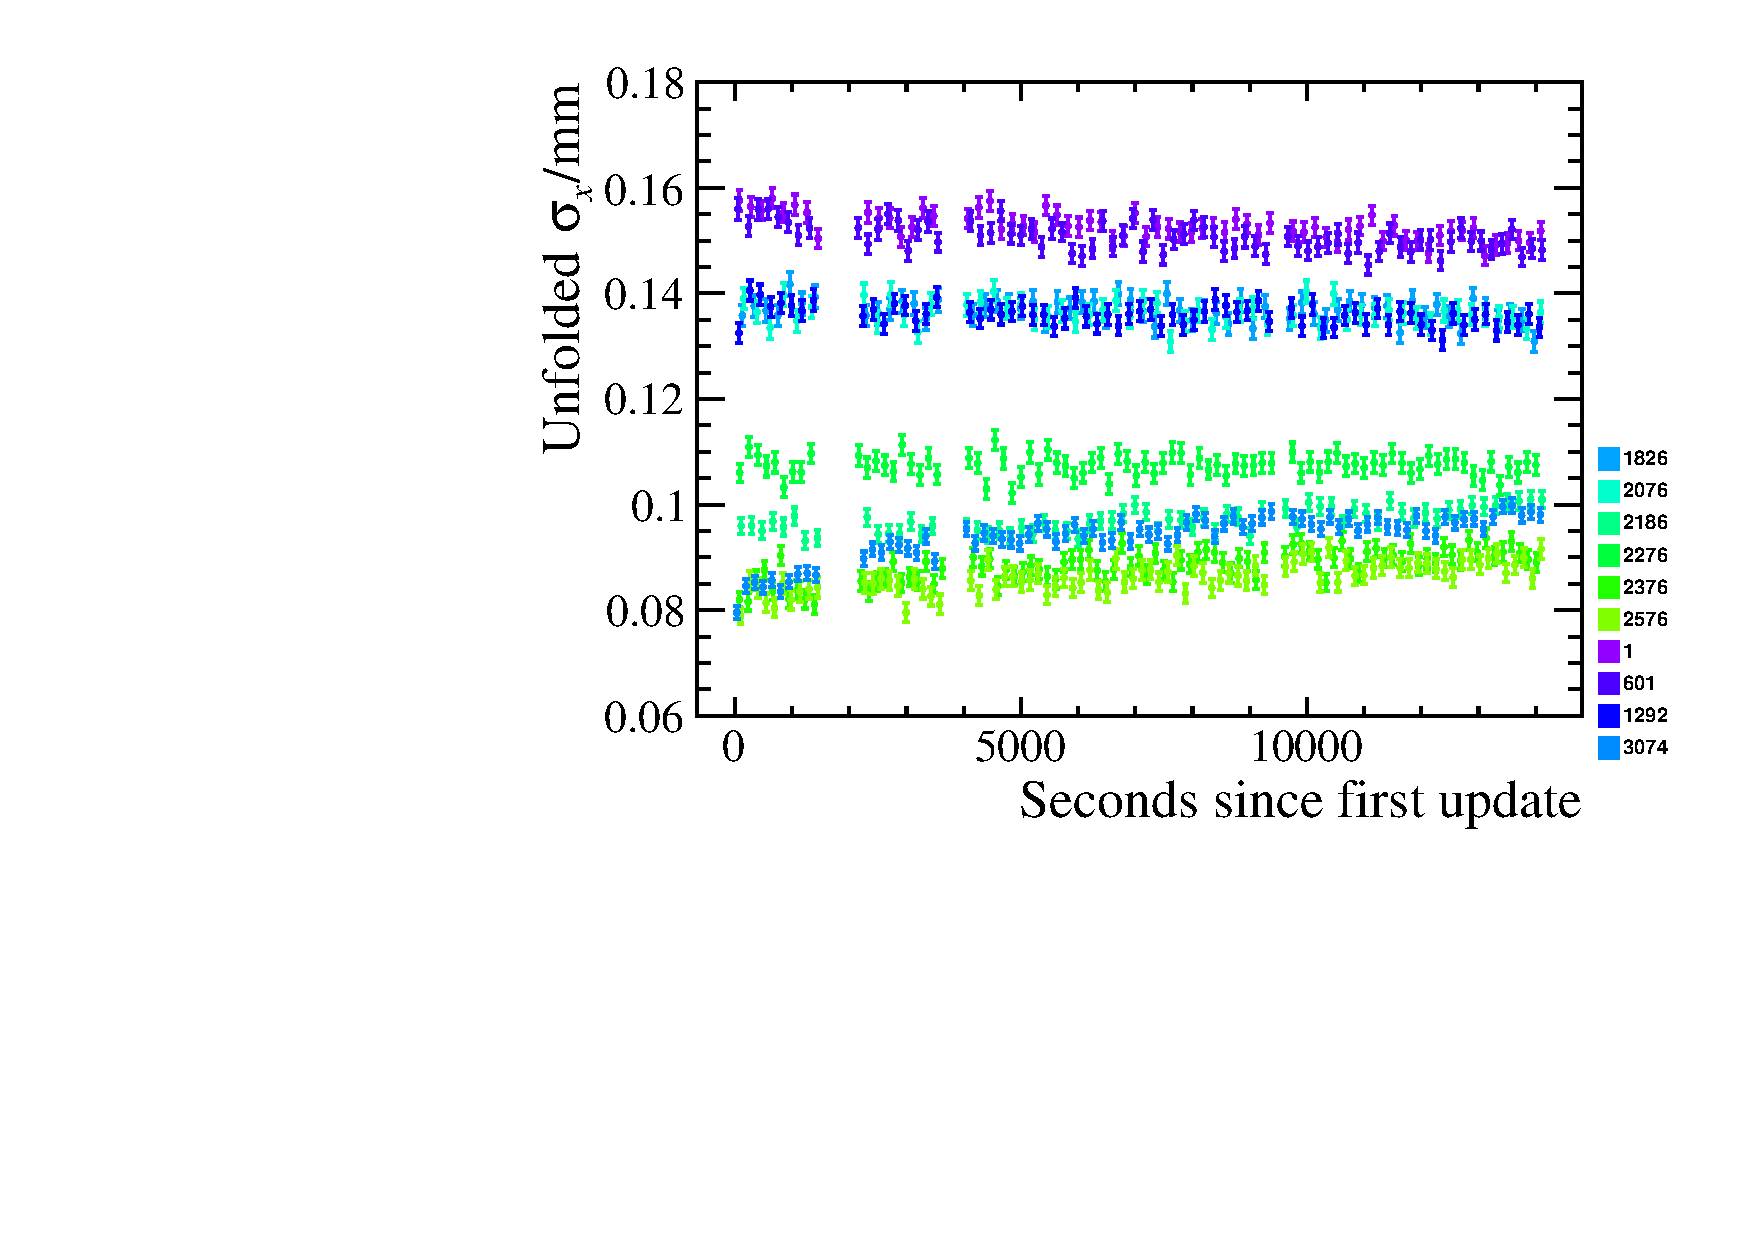
\includegraphics[width=1.0\textwidth]{figs/Detector/PerBXID_SigmaX_unfolded_Beam1.pdf}
    \end{subfigure}
    \caption{The mean position (left) and width (right) of individual Beam 1 bunches in the $x$-dimension. These values have been corrected for the \velo resolution. The beam optics were designed to have a large range of bunch sizes.}
    \label{fig:Dec_bgi_fill}   
\end{figure}
%%%%%%%%%%%%%%%%%%%%%%%%%%%%%%%%%%%%%%%%%%%%%%%%%%%%%%%%%%



